%% -*- coding: utf-8; -*-

\documentclass[phd,american]{ThesisPUC}

%---------- Math ----------%
\usepackage{amsmath}
\usepackage{amssymb}
\usepackage{mathtools}
\usepackage{bbm}
%\usepackage{ulem}
%---------- Floting ----------%
\usepackage{float}
% ---------- References ----------%
%\usepackage[sort&compress,round,comma,numbers]{natbib}
%\usepackage{natbib}
% ---------------------------------------
% author: Alan Livio
% site: github.com/alanlivio/latex-helper-functions
% ---------------------------------------

% ----------------------------------------
% work like layout
% ----------------------------------------
% \usepackage{wordlike}
% \usepackage[big]{layaureo}

% ----------------------------------------
% ABNT like layout
% ----------------------------------------
% \usepackage{lmodern}
% \setlength{\parskip}{0.2cm}
% \setlength{\parindent}{1.3cm}
% \usepackage{geometry}
%  \geometry{
%  a4paper,
%  total={170mm,257mm},
%  left=3cm,
%  top=3cm,
%  right=3cm,
%  bottom=3cm
%  }

% ----------------------------------------
% SmallCaps font
% ----------------------------------------
% \usepackage{fontspec}
% \defaultfontfeatures{Mapping=tex-text}
% \setmainfont[
% SmallCapsFont = Fontin-SmallCaps.otf,
% BoldFont = Fontin-Bold.otf,
% ItalicFont = Fontin-Italic.otf
% ]{Fontin.otf}

% ----------------------------------------
% language
% ----------------------------------------
\usepackage[brazilian, american]{babel}
% \usepackage[portuguese]{babel}

% ----------------------------------------
% fonts
% ----------------------------------------
\usepackage[T1]{fontenc}
\usepackage[utf8]{inputenc}
\usepackage{textcomp}
\usepackage{amsmath,amssymb,amsfonts}

% ----------------------------------------
% tables
% ----------------------------------------
\usepackage{makecell}
\usepackage{tabularx}
\usepackage{multirow}
%\usepackage[nottoc]{tocbibind}

% ----------------------------------------
% table custom cells
% ----------------------------------------
\newcolumntype{L}[1]{>{\raggedright\arraybackslash}p{#1}}
\newcolumntype{C}[1]{>{\centering\arraybackslash}p{#1}}
\newcolumntype{R}[1]{>{\raggedleft\arraybackslash}p{#1}}

% ----------------------------------------
% URL and hyperref
% ----------------------------------------
%\usepackage[hyphens]{url}
%\usepackage{hyperref}
%\hypersetup{hidelinks}

% ----------------------------------------
% URL color
% ----------------------------------------
% \definecolor{linkcolour}{rgb}{0,0.2,0.6}
% \hypersetup{colorlinks,urlcolor=linkcolour, linkcolor=linkcolour}

% ----------------------------------------
% includegraphics
% ----------------------------------------
\usepackage{graphicx}

% ----------------------------------------
% includegraphics for larging image with subcaption
% ----------------------------------------
\usepackage{float}
\usepackage{newfloat}
\usepackage{subfloat}
\usepackage{subcaption}

% ----------------------------------------
% itemize
% ----------------------------------------
\usepackage{enumitem}
\SetEnumitemKey{mynosep}{noitemsep, nosep, topsep=0pt, partopsep=0pt, parsep=0pt, itemsep=0pt, leftmargin=*}
\def\labelitemi{$-$}

% ----------------------------------------
% color
% ----------------------------------------
\RequirePackage{color}
\usepackage{soulutf8}
\usepackage{xcolor}
\usepackage{multicol}

\colorlet{light-gray}{gray!20}
\usepackage{listings}
\DeclareFloatingEnvironment[fileext=lst,placement={!htbp},name=Listing]{listing}

\usepackage{color}
\definecolor{dkgreen}{rgb}{0,0.6,0}
\definecolor{gray}{rgb}{0.5,0.5,0.5}
\definecolor{mauve}{rgb}{0.58,0,0.82}
\definecolor{gray}{rgb}{0.4,0.4,0.4}
\definecolor{darkblue}{rgb}{0.0,0.0,0.6}
\definecolor{lightblue}{rgb}{0.0,0.0,0.9}
\definecolor{cyan}{rgb}{0.0,0.6,0.6}
\definecolor{darkred}{rgb}{0.6,0.0,0.0}

\renewcommand{\ttdefault}{pcr}
\lstset{
  basicstyle=\ttfamily\footnotesize,
  columns=fullflexible,
  showstringspaces=false,
  numbers=left,                   % where to put the line-numbers
  numberstyle=\tiny\color{gray},  % the style that is used for the line-numbers
  stepnumber=1,
  numbersep=5pt,                  % how far the line-numbers are from the code
  backgroundcolor=\color{white},      % choose the background color. You must add \usepackage{color}
  showspaces=false,               % show spaces adding particular underscores
  showstringspaces=false,         % underline spaces within strings
  showtabs=false,                 % show tabs within strings adding particular underscores
  frame=none,                   % adds a frame around the code
  rulecolor=\color{black},        % if not set, the frame-color may be changed on line-breaks within not-black text (e.g. commens (green here))
  tabsize=2,                      % sets default tabsize to 2 spaces
  captionpos=b,                   % sets the caption-position to bottom
  breaklines=true,                % sets automatic line breaking
  breakatwhitespace=true,        % sets if automatic breaks should only happen at whitespace
  title=\lstname,                   % show the filename of files included with \lstinputlisting;
                                  % also try caption instead of title  
  commentstyle=\color{gray}\upshape
}


\lstdefinelanguage{XML}
{
  morestring=[s][\color{black}]{"}{"},
  morestring=[s][\color{black}]{>}{<},
  morecomment=[s]{<?}{?>},
  morecomment=[s][\color{dkgreen}]{<!--}{-->},
  stringstyle=\color{black},
  identifierstyle=\color{darkgray}\bfseries,
  keywordstyle=\color{black},
  morekeywords={xmlns,xsi,noNamespaceSchemaLocation,type,id,x,y,source,target,version,tool,transRef,roleRef,objective,eventually}% list your attributes here
}


% ----------------------------------------
% fixme
% ----------------------------------------
\usepackage[nomargin,inline]{fixme}
\fxusetheme{color}
% \fxsetup{draft}
% \fxsetup{final}

% ----------------------------------------
% ref elements
% ----------------------------------------
\newcommand{\reffig}[1]{\figurename~\ref{#1}}
\newcommand{\reftab}[1]{Table~\ref{#1}}
\newcommand{\reflis}[1]{Listing~\ref{#1}}
\newcommand{\refappen}[1]{Appendix~\ref{#1}}
\newcommand{\refsec}[1]{Section~\ref{#1}}
\newcommand{\refsubsec}[1]{subsection~\ref{#1}}

% ----------------------------------------
% xml tags
% ----------------------------------------
\newcommand{\xml}[1]{\texttt{<#1>}}
\newcommand{\attr}[1]{\emph{#1}}

% ----------------------------------------
% compact section titles
% ----------------------------------------
% \usepackage[compact]{titlesec}
% \titlespacing{\section}{0pt}{*0}{*0}
% \titlespacing{\subsection}{0pt}{*0}{*0}
% \titlespacing{\subsubsection}{0pt}{*0}{*0}

% ----------------------------------------
% for
% ----------------------------------------
\usepackage{forloop}

% spacing control
% ----------------------------------------
% \setlength{\itemsep}{0pt}
% \setlength{\parskip}{0pt}
% \setlength{\parsep}{0pt}
% \setlength{\abovecaptionskip}{1pt}
% \setlength{\belowcaptionskip}{1pt}

% ----------------------------------------
% lipsum
% ----------------------------------------
\usepackage{lipsum}

% ----------------------------------------
% tree
% ----------------------------------------
\usepackage{tikz}
\usetikzlibrary{trees}

% % ----------------------------------------
% % minted listing inside tcolorbox
% % ----------------------------------------
% \usepackage{listings}
% \usepackage{tikz}
% \usepackage[many]{tcolorbox}
% \usepackage{minted}
% \tcbuselibrary{minted,breakable,skins,raster}
% \newtcblisting[]{mintedlistingtcblisting}[1][!ht]{
%   enhanced jigsaw,pad at break*=5mm,
%   fontsize=\footnotesize
%   colback=yellow!5,colframe=yellow!50!black,listing only,
%   listing engine=minted,
%   minted language=#1,
%   minted options={fontsize=\footnotesize,breaklines,autogobble,linenos,numbersep=3mm},
%   overlay={\begin{tcbclipinterior}\fill[red!20!blue!20!white] (frame.south west)
%   rectangle ([xshift=5mm]frame.north west);\end{tcbclipinterior}}
% }

% ----------------------------------------
% listing code inside tcolorbox
% ----------------------------------------
\usepackage{listings}
\usepackage[many]{tcolorbox}
\tcbuselibrary{listingsutf8}
\newtcblisting[]{mytcblisting}[1][!ht]{
  enhanced jigsaw,
  enforce breakable,
  pad at break*=1mm,
  colback=black!2,
  colframe=black!30,
  top=1mm, bottom=1mm, left=0mm, right=0mm,
  listing only,
  coltitle=black,
  % drop fuzzy shadow,
  listing options={
    % shape
    xleftmargin=0pt, % 0 is default
    xrightmargin=-4pt, % 0 is default
    % frame ---
    framesep=0pt,
    aboveskip=-6pt,
    belowskip=-6pt,
    captionpos=b, % sets the caption position
    % numbers ----
    % numberstyle=\footnotesize\ttfamily,
    numbers=left,
    % firstnumber=2
    numbersep=8pt,% how far the line-numbers are from the code
    stepnumber=1, % the step between two line-numbers.
    numberstyle=\tiny\ttfamily,
    % code ----
    language=#1,
    tabsize=2,
    showspaces=false, % show spaces with underscores
    showstringspaces=false, % underline spaces within strings
    showtabs=false, % show tabs using underscores
    breaklines=true, % sets automatic line breaking
    breakindent=8pt,
    basicstyle=\footnotesize\ttfamily,
    columns=fullflexible,
    keywordstyle=\color{black},
    morekeywords={
      <, >,
    },
  },
}

% ----------------------------------------
% draft watermark
% ----------------------------------------
\newcommand\enableDraftWatermark{
  \RequirePackage{draftwatermark}
  \SetWatermarkFontSize{0.5in}
  \SetWatermarkColor[gray]{.9}
  \SetWatermarkText{\parbox{12em}{\centering
      Unpublished working draft.\\
      Not for distribution.}}
}


% ----------------------------------------
% acm prepring
% ----------------------------------------
\newcommand\enableACMPreprint{
  \settopmatter{printacmref=false}
  \setcopyright{none}
  \renewcommand\footnotetextcopyrightpermission[1]{}
  \pagestyle{plain}
}

% ----------------------------------------
% blind review authors
% ----------------------------------------
\newcommand\addACMBlindReviewAuthors{
  \author{Removed for double-blind review}
  \affiliation{%
    \institution{Removed for double-blind review}}

  \author{Removed for double-blind review}
  \affiliation{%
    \institution{Removed for double-blind review}}

  \author{Removed for double-blind review}
  \affiliation{%
    \institution{Removed for double-blind review}}

  \renewcommand{\shortauthors}{Removed for double-blind review}
}

\newcommand\addIEEEBlindReviewAuthors{
  \author{
  \IEEEauthorblockN{Removed for double-blind review}
  \IEEEauthorblockA{Removed for double-blind review  \\ Removed for double-blind review}
  \and
  \IEEEauthorblockN{Removed for double-blind review}
  \IEEEauthorblockA{Removed for double-blind review  \\ Removed for double-blind review}
  \and
  \IEEEauthorblockN{Removed for double-blind review}
  \IEEEauthorblockA{Removed for double-blind review  \\ Removed for double-blind review}
  }
}

%---------- Algorithm ----------%
\usepackage{algorithm}
\usepackage{algpseudocode}

\PassOptionsToPackage{noend}{algpseudocode}%comment out if want end's to show

\errorcontextlines\maxdimen

% begin vertical rule patch for algorithmicx (http://tex.stackexchange.com/questions/144840/vertical-loop-block-lines-in-algorithmicx-with-noend-option)
\makeatletter
% start with some helper code
% This is the vertical rule that is inserted
\newcommand*{\algrule}[1][\algorithmicindent]{\makebox[#1][l]{\hspace*{.5em}\vrule height .75\baselineskip depth .25\baselineskip}}%

\newcount\ALG@printindent@tempcnta
\def\ALG@printindent{%
    \ifnum \theALG@nested>0% is there anything to print
        \ifx\ALG@text\ALG@x@notext% is this an end group without any text?
            % do nothing
            \addvspace{-3pt}% FUDGE for cases where no text is shown, to make the rules line up
        \else
            \unskip
            % draw a rule for each indent level
            \ALG@printindent@tempcnta=1
            \loop
                \algrule[\csname ALG@ind@\the\ALG@printindent@tempcnta\endcsname]%
                \advance \ALG@printindent@tempcnta 1
            \ifnum \ALG@printindent@tempcnta<\numexpr\theALG@nested+1\relax% can't do <=, so add one to RHS and use < instead
            \repeat
        \fi
    \fi
    }%
\usepackage{etoolbox}
% the following line injects our new indent handling code in place of the default spacing
\patchcmd{\ALG@doentity}{\noindent\hskip\ALG@tlm}{\ALG@printindent}{}{\errmessage{failed to patch}}
\makeatother
% end vertical rule patch for algorithmicx    

%---------- Tables ----------%
\usepackage{multicol}
\usepackage{booktabs}
\usepackage{colortbl}
\usepackage{tabularx}
%---------- TiKz ----------%
\usepackage{threeparttable}
\usepackage{standalone}
\usepackage{xcolor}
\usepackage{tikz}
\usepackage{psfrag,epsf}
\usepackage{multirow}
\usepackage{listings}
\usepackage{soul}
%----------citation------------%
%\usepackage{apacite}

%-----------color-----------------%
\definecolor{dkblue}{rgb}{0,0,.6}
\definecolor{turquoise}{rgb}{0.25,0.87,0.82}
\definecolor{dkgreen}{rgb}{0,0.6,0}
\definecolor{dkred}{rgb}{0.7,0,0}
\definecolor{indigo}{rgb}{0.294, 0, 0.51}
\definecolor{cyan}{rgb}{0, 0.70, 0.70}
\definecolor{gray}{rgb}{0.5,0.5,0.5}
\definecolor{mauve}{rgb}{0.58,0,0.82}
\definecolor{black}{rgb}{0,0,0}

\newcommand{\pmendes}[1]{\color{red}\textbf{paulo says: }#1\color{black}}


%\pagestyle{plain}


%Para o código em EPL
\lstdefinestyle{EPLStyle}{
  numbers=left,
  numberstyle=\footnotesize\ttfamily,
  language=SQL,
  frame=tblr,
  aboveskip=0mm,
  belowskip=3mm,
  showstringspaces=false,
  columns=flexible,
  basicstyle={\small\ttfamily},
  numberstyle=\tiny\color{gray},
  keywordstyle=\color{blue},
  commentstyle=\color{gray},
  stringstyle=\color{dkgreen},
  breaklines=true,
  breakatwhitespace=true,
  tabsize=3,
  %Adiciona as keywords específicas da EPL Esper
  morekeywords={after, at, context, current_timestamp,  define, distinct, every, first, grouping, grouping_id, hour, hours, initiated, inner, instanceof, irstream, is, istream, last, match_recognize,  measures, min, minute, minutes, microsecond, microseconds, millisecond, milliseconds, msec, new, offset, output, partition, pattern, rstream, sec, second, seconds, sets, some, snapshot, sql, start, terminated, then, until, usec, using, variable, weekday, when, while, window, schema},
%
  frameround=tttt,
}

\graphicspath{{images/}}

% ---------- Cover ----------%
% Adjust the advisor's title according to gender(Prof. or Prof$^{\text{a}}$.)
\author{Paulo Renato Conceição Mendes}
\authorR{Mendes, Paulo Renato Conceição}
\advisor{Sérgio Colcher}{Prof.}
\advisorR{Colcher, Sérgio}

% This thesis will use colored figures, this goes in the catalographic sheet
\usecolour{true}
\title{Spatiotemporal Localization of Actors   in Video/360-Video and its Applications}

\titleuk{Spatiotemporal Localization of Actors in Video/360-Video and its Applications}

\day{27$^{th}$}
\month{July}
\myyear{2021}

% CDD is the registry number of the area, given by the library. Our area (informatics) is 004.
\city{Rio de Janeiro}
\CDD{004}
\department{Informática}
\program{Informática}
\school{Centro Técnico Científico}
\university{Pontifícia Universidade Católica do Rio de Janeiro}
\uni{PUC-Rio}

%---------- Jury ----------%

% Internal jury members are declared with \jurymember{name}{title}{department}{university}
% external jury members are declared with \extjurymember{name}{title}{university}
\jury{
  \jurymember{Alberto Barbosa Raposo}{Prof.}{Departamento de Informática}{PUC-Rio}
  \extjurymember{Roberto Gerson de Albuquerque Azevedo}{Dr.}{Disney Research}
}

%---------- Front letters ----------%
\resume
{
Bachelor's degree in Computer Science at Federal University of Maranhão (UFMA) in 2019.
}

\acknowledgment
{
\noindent
Thanks to my advisor Prof. Sérgio Colcher for his guidance and support in this journey.
Thanks to my family for the endless support.
Thanks to my friends from TeleMídia Lab, for their friendship and support. To all colleagues, faculty and staff of the PUC Rio Department of Informatics for the fellowship, learning and support.
This study was financed in part by the Coordenação de Aperfeiçoamento de Pessoal de Nível Superior - Brasil (CAPES) - Finance Code 001.
}


% Workaround for keywords. The keywords in the catalographic sheet must be separated by dots, while the ones shown in the abstract must be separated by semi-colons.
% Thats why we have two commands for each language: \keywords declares the keywords for the catalographic sheet, while \keywordsabstract declares the ones for the abstract.
\keywords
{
  \key{Clusterização}
  \key{Reconhecimento Facial}
  \key{Recomendação de Vídeo}
  \key{Vídeo 360}
  
  
}

\keywordsabstract
{
  \key{Clusterização;}
  \key{Reconhecimento Facial;}
  \key{Recomendação de Vídeo;}
  \key{Vídeo 360.}
}

\keywordsuk
{

  \key{Clustering}
  \key{Face Recognition}
  \key{Video Recommendation}
  \key{360-Video}
}

\keywordsabstractuk
{
  \key{Clustering;}
  \key{Face Recognition;}
  \key{Video Recommendation;}
  \key{360-Video.}
}

\abstract{
  A disseminação atual da IoT aumenta a implantação de soluções de processamento de fluxo de dados para monitorar e controlar elementos do mundo real. Uma dessas soluções é o Processamento de Eventos Complexos (CEP). Inicialmente, um único computador ou cluster concentraria toda a execução do CEP. No entanto, a execução centralizada do CEP não é ideal para lidar com o alto volume, velocidade e volatilidade dos fluxos de dados dos sensores IoT. Em vez disso, as aplicações CEP devem criar e decentralizar o processamento de eventos CEP, de preferência tendo agentes CEP na nuvem e em dispositivos na borda. Além disso, tão importante quanto a descentralização, é decidir como o processamento será dividido entre esses dispositivos. Dito isso, estar ciente do contexto atual de cada dispositivo, por exemplo, sua localização e sensores disponíveis, pode ajudar a coletar e (parcialmente) processar os dados em dispositivos próximos ao local onde os dados foram produzidos. Este trabalho apresenta uma plataforma de CEP distribuído com ciência de contexto chamada Global CEP Manager (GCM). GCM é um serviço do middleware ContextNet que oferece suporte à implantação e ao rearranjo dinâmico de consultas CEP baseados em contexto para motores CEP em execução na nuvem, em dispositivos na borda estacionários e M-Hubs, que são dispositivos na borda móveis do ContextNet. O GCM usa o ContextMatcher, que também faz parte deste trabalho. ContextMatcher é um módulo para aplicações ContextNet que permite a entrega de mensagens para nós cujo contexto esteja de compatível com um determinado conjunto de características contextuais.
}

\abstractuk{
  The current dissemination of IoT increases the deployment of stream processing solutions for monitoring and controlling elements of the real world. One of those solutions is Complex Event Processing (CEP). Initially, a single computer/cluster would concentrate all the CEP execution. However, a centralized execution of CEP is not suitable for coping with the high volume, velocity, and volatility of IoT sensors’ data streams. Instead, applications using CEP should deploy a distributed CEP Event Processing Network, preferably having CEP agents both in the cloud and at edge devices. Also, deciding the arrangement used to split the processing among these tiers and their devices can be just as important. That said, being aware of each of the devices’ current context, for instance, their location and available sensors, can help to collect and (partially) process the data on devices close to the data’s production site. This work presents a context-aware distributed CEP platform called Global CEP Manager (GCM). GCM is a service of the ContextNet middleware that supports the context-based deployment, and dynamic rearrangement of CEP queries to CEP engines executing in the cloud, stationary edge devices, and  M-Hubs, which are ContextNet’s mobile edge devices. GCM uses the ContextMatcher, which is also part of this work. ContextMatcher is a module for ContextNet applications that enables the delivery of messages for nodes that match a specified set of contextual requirements.
}


% WARNING
% The epigraph, if present, must come before the first chapter, always.
% There is a list of abreviations (abrevs.tex) which is included automatically in the ThesisPUC.cls, and is optional, comment the %% -*- coding: utf-8; -*-

\begin{thenotations}
\renewcommand{\arraystretch}{1.5}
  \noindent
  \begin{tabular}{ll}

CNN -- Convolutional Neural Network\\
FDDB -- Face Detection Data set and Benchmark\\
FOV -- Field of View\\
FRPC -- Face Recognition Prize Challenge\\
GTP -- Ground Truth Positives\\
HMD -- Head-Mounted Display\\
HOG -- Histogram of Oriented Gradients\\
HTML -- HyperText Markup Language\\
HUD -- Heads-up Display\\
IARPA -- Intelligence Advanced Research Projects Activity\\
IJB -- IARPA Janus Benchmark-B\\
LFW -- Labeled Faces in the Wild\\
MAP -- Mean Average Precision
MOOC -- Massive Open Online Course\\
MTCNN -- Multitask Cascaded Convolutional Networks\\
NAN -- Neural Aggregation Network\\
NCL -- Nested Context Language\\
NMS -- Non-Maximum Suppression\\
PIP -- Picture-in-Picture\\
SMIL -- Synchronized Multimedia Integration Language\\
SRT -- SubRip Subtitle Format\\
VR -- Virtual Reality\\
VTE -- Virtual Teaching Environment\\
XML -- Extensible Markup Language\\

  \end{tabular}

\end{thenotations} line if you do not wish to included it.
% Rationale: In the original template, the list of abreviations came before the epigraph, which caused problems with the university library, thus I've included it in the cls file.
% TODO: Declare a boolean option in the ThesisPUC.cls class in order to selectively include the abreviations list.

%%%%%%%%%%%%%%%%%%%%%%%%%%%%%%%%%%%%%%%%%%%%%%%%%%%%%%
\begin{document}

%%% -*- coding: utf-8 -*-
\newpage

\chapter{Introduction}
\label{chap:introduction}

In recent years, the popularity of platforms for the storage and transmission of video content has stimulated the production of a massive volume of video data, establishing new habits, and leveraging new applications with innovative forms of consumption of this kind of information. Just as an indication of this huge production (and consumption) of data, we mention that, in 2019, for example, more than one billion hours of YouTube videos were watched per day.\footnote{https://kinsta.com/blog/youtube-stats/}


Generating metadata with (i) the identity information of actors present, (ii) the temporal determination of the intervals in which each of these actors is present, and (iii) their spatial localization in each of the frames along these intervals can facilitate video indexing, retrieval, recommendation and a series of other tasks which might enhance the way people interact and consume all this video data. Besides the identification, (ii) and (iii) together are what we call \textit{Spatiotemporal Localization}. 

In this dissertation, we investigate a method for the spatiotemporal localization of actors in videos. Our expected contribution is two-fold: 
\begin{enumerate}
\item we propose a core process for the spatiotemporal localization in which we take advantage of face detection, embeddings, and clustering methods to group similar faces (presumably from the same actors) along with the frames, and \item we further explore, propose and investigate the innovative application of this localization in three different practical and important tasks: \emph{Video Face Recognition}, \emph{Educational Video Recommendation}, and \emph{Subtitles Positioning in 360-video}.  
\end{enumerate}

The common core of this dissertation relies on its first part, in which we describe a \textit{Video Face Clustering} method for the spatiotemporal localization of actors. We describe its process composed of: \textit{frame extraction}, \textit{face detection}, \textit{embeddings generation} and \textit{clustering}. 

Based on this \emph{Video Face Clustering} method, we investigate three chosen applications in which we explore novel approaches, all of them enabled by that common method of localization and its benefits. 

The first application, that of \emph{Video Face Recognition}, has been attracting the attention of researchers for more than two decades. Since the deep learning boom, face detection and recognition performance have greatly improved in terms of both speed and accuracy~\cite{masi2018deep}. Nowadays, face recognition systems are used in many areas such as video surveillance and security systems, video analytics systems, smart shopping, automatic face tagging in photo collections, investigative tools that search for identities in social networks based on face images, and in thousands of other applications in our daily lives.

In our work, we propose a \textit{cluster-matching-based approach} for \emph{Video Face Recognition} where clustering is used to group faces in both the face dataset and in the target video. This method was motivated (and made possible) mainly by the characteristics of our core \emph{Video Face Clustering} method. Its main benefit is that classes (which represent different actors) do not have to be previously known, so the effort spent with annotations is significantly reduced --- as it is done over clusters instead of single images. Consequently, face recognition becomes a task of comparing clusters from the dataset with the ones extracted from images or video sources. Therefore, our approach is easily scalable and can be used to automatically generate video metadata.

The second application, that of \emph{Educational Video Recommendation}, may be considered as one of a more general class of applications referenced as \textit{recommendation system applications} and was motivated by a shift of paradigms that we have been observing in recent years. The traditional paradigm of classroom courses, centered on the physical presence of a teacher, has been gradually giving space to online and hybrid courses, which enables the emergence of VTEs (Virtual Teaching Environment) and MOOCs~(\textit{Massive Open Online Courses}).
If, on the one hand, the abundance of educational videos can contribute to and facilitate learning, on the other hand, it also makes it challenging to discover and access some specific content of interest~\cite{dias2017approach}.
This issue is usually addressed by a proactive user search (using queries, for example), or by automatic recommendations made by specialized systems.


In general, current video recommendation methods are heavily dependent on textual information from the video, such as labels (\textit{i.e.} keywords)~\cite{mahajan2015optimising,omisore2014personalized}, or automatically generated captions \cite{barrere2020utilizaccao} from the lecturer speech. These systems face problems such as errors introduced by manually inserted labels or by imprecise speech recognition.
In this work, we propose an additional feature to enhance the recommendation of educational video content which is based on actors~(in this specific case, lecturers) presence. To do that, again we take advantage of our core \emph{Video Face Clustering} method. More precisely, we detect lecturers in a video taken as a reference and perform a clustering based on the face of these lecturers in different videos. Given these clusters, we extract their \textit{centroids} and perform another clustering step for creating a relationship between videos that share the presence of the same lecturers. Finally, we rank the recommended videos based on the amount of time the referenced lecturers were present.
A particular benefit of this approach is that it can be done without supervision, allowing for new videos to be automatically analyzed.

Our third application (\emph{Subtitles Positioning in 360-Video}) was motivated by the recent popularization of omnidirectional cameras and Head-Mounted-Displays (HMDs) that increased the amount of 360-video content available. Omnidirectional videos are spherical visual signals that allow the viewer to look around a full 360-degree view of a scene from a specific point.

Several people use subtitles when consuming audiovisual media, and these subtitles are important in contributing to the understanding of the video content \cite{brown_subtitles_2017}. Some people choose to consume videos muted \cite{hughes_disruptive_2019}. Additionally, the work of \cite{hayati2011effect}, as referenced in \cite{hughes_disruptive_2019}, shows that consumers are more likely to watch videos entirely if they have subtitles presented with them. In traditional 2D videos, static subtitles are commonly used and they are usually placed at a fixed position, most commonly at the bottom-center of the screen \cite{rothe_dynamic_2018}.
Different from traditional 2D videos, subtitles positioning in 360-videos is challenging because it involves both temporal and spatial domains \cite{agullo2019making}, and there is no fixed ``bottom-center" of the screen \cite{brown_subtitles_2017}. Most current solutions rely on positioning subtitles either statically to the viewer or at a fixed position in the 360-degree environment. 
In this work, we adapt and apply our current solution for the spatiotemporal localization of actors to the 360-video domain. By doing that, we intend to use this localization for positioning subtitles close to the actors in the 360-video.

The remainder of this dissertation proposal is structured as follows. 
In Chapter \ref{chap:related}, we discuss some works related to the core method of our dissertation and each of the applications we investigate.
In Chapter \ref{chap:video_face_clustering}, we define our approach for spatiotemporal localization of actors, which is our core method.
The following three chapters contain the applications in which we investigate the applicability of this method.
The first application, that of \emph{Video Face Recognition}, is described in Chapter \ref{chap:face_recognition}.
In Chapter \ref{chap:educational_recommendation}, we present our application of \emph{Educational Video Recommendation}.
Our last application, that of \emph{Subtitles Positioning in 360-video}, is described in Chapter \ref{chap:subtitles_positioning}. Finally, in Chapter \ref{chap:conclusions}, we conclude this dissertation and point to possible future work.
%%% -*- coding: utf-8 -*-
\newpage

\chapter{Related Work}
\label{chap:related}

In this chapter we make a brief review of the works related to ours. Section \ref{sec:spatiotemporal} contains works related to the core method of this word. The next three sections describe works related to the applications we propose based on our core method.

\section{Spatiotemporal Localization of Actors}
\label{sec:spatiotemporal}


The task of detecting and tracking actors in video has been the focus of many researches. In early 2004, \cite{facetracking_2} used an illumination invariant approach for face detection combined with a tracking mechanism performed by means of continuous detections. \cite{face_tracking} addressed the problem of tracking faces in noisy videos using a tracker that adaptively builds a target model reflecting changes in appearance, typical of a video setting. This kind of approaches does not perform well in the task of spatiotemporal localization of actors because they can only track them when they are continuously present on the video. Differently, the approach we use, which is based on clustering, does not require the actors to be continuously present on the video.

More similar to ours, recent works have investigated the use of clustering for grouping faces of actors in video and, consequently, providing the spatiotemporal localization of them. \cite{video_face_clustering} propose Ball Cluster Learning~(BCL), a supervised approach to carve the embedding space into balls of equal size, one for each cluster. The radius of such ball is translated to a stopping criterion for iterative merging algorithms. \cite{self_supervised} propose a self-supervised Siamese network for video face clustering that can also be used in scenarios where tracks of actors are not available, such as image collections. The approach we use can also be applied to image collections, as further explained in Section \ref{chap:face_recognition}, but it differs in the sense that we use pre-trained CNNs and traditional clustering algorithms for performing this task. 

It is worth mentioning that, in this dissertation, we do not intend to directly compare or propose a better method for the task of spatiotemporal localization of actors than the existing ones. Instead, we intend to investigate in what extent our method opens up novel approaches for the three chosen applications and the benefits that can be achieved with our approach.

\section{Video Face Recognition}
\label{sec:video_face}

Many methodologies have been proposed for Video Face Recognition, most commonly relying on comparing selected facial features of a given image with features of faces within a database.
%%
Using only one sample reference image of a person's face for the comparison may result in classification errors due to factors related to variations in lighting, image resolution, angle, etc.~\cite{598229}.
%%
To overcome this problem, some face recognition approaches use multiple face samples for comparison. However, this strategy does not scale well as the complexity is a function of the number of samples.
%%
Other approaches treat the face recognition task as a classification problem~\cite{dadi2016improved, ghosal}, where a classifier model learns rules to assign faces to previously known classes within a dataset, where each class corresponds to one person.
%%
Nonetheless, this kind of approach does not deal well when new classes are incorporated because of the need to retrain the classification models.
%%
Moreover, when dealing with video, these kinds of methods have to be applied to each frame, again increasing the complexity.


Traditional deep learning models for face recognition such as DeepFace~\cite{taigman2014deepface} and DeepID~\cite{sun2014deep} use a CNN with fully-connected layer output to produce a representation of high-level features (face embeddings) from an input image, followed by a softmax layer to indicate the identity of classes. Other approaches, such as FaceNet~\cite{schroff2015facenet}, can directly measure the similarity among faces using euclidean space. Inspired by DeepID, this model uses the \textit{triplet loss} as the loss function to estimate similarity to one character's face to a  collection of other faces. Triplet loss improves the accuracy of the  CNN output by minimizing the euclidean distance between the anchor and the positive (face of the same identity) while maximizing the distance between the anchor and the negative (face of another identity). In this work, we evaluated different pre-trained CNN backbones on VGGFace2 dataset~\cite{cao2018vggface2} to generate the face embeddings. This model is the state-of-the-art\footnote{https://paperswithcode.com/paper/vggface2-a-dataset-for-recognising-faces} in the face verification task on the IJB-B dataset~\cite{whitelam2017iarpa}. 


Proprietary systems for face recognition and matching are widely used by social network platforms. For instance, Facer~\cite{hazelwood2018applied} is Facebook's face detection and recognition framework. Given a photograph, it first detects all the faces. Then, it runs a  deep model to determine the likelihood of that face belonging to one of the top-N user friends. This allows  Facebook to suggest which friends the user might want to tag within the uploaded photographs. FindFace\footnote{https://findface.br.aptoide.com/app} is an app that matches photos to profile pictures on VKontakte,\footnote{https://vk.com/} a Russian social networking website similar to Facebook. FindFace uses a deep model developed by NTech Lab that won the \textit{2017 IARPA Face Recognition Prize Challenge} (FRPC)~\cite{grother20172017}  in two nominations out of three (“Identification Speed” and “Verification Accuracy”). Similarly, our method can detect faces in videos and automatically recognize their identities by a clustering-based algorithm that uses a knowledge base with the faces pre-identified as a reference; however, a comparison with such methods was not possible due to access restrictions.

Some recent works are focused on video face recognition. Pena \textit{et al.}~\cite{globofacestream} proposed a face recognition system to detect characters within videos, called~\textit{Globo Face Stream}. Their method uses a Histogram of Oriented Gradients (HOG) feature combined with a linear classifier to detect faces. Next, they use  FaceNet to generate the embeddings, followed by the euclidean distance calculus to measure the similarity among faces. Yang \textit{et al.}~\cite{yang2017neural} proposed a deep network for video face recognition called NAN (Neural Aggregation Network). They use a CNN to generate the embeddings, followed by an aggregation module that consists of two attention blocks which adaptively aggregate the feature vectors to form a single feature inside the convex hull spanned by them. Rao \textit{et al.}~\cite{rao2017attention} proposed a method for video face recognition based on attention-aware deep reinforcement learning. They formulated the process of finding the attention of videos as a Markov decision process and training the attention model without using extra labels. Unlike existing attention models, their method takes information from both the image space and the feature space as the input to make use of face information that is discarded in the feature learning process. Sohn \textit{et al.}~\cite{sohn2017unsupervised} proposed an adaptative deep learning framework for image-based face recognition and video-based face recognition. Given an embedding generated by a CNN, their framework adaptation is achieved by (1) distilling knowledge from the network to a video adaptation network through feature matching, (2) performing feature restoration through synthetic data augmentation, and (3) learning a domain-invariant feature through an adversarial domain discriminator. 

Like~\cite{globofacestream, yang2017neural, rao2017attention, sohn2017unsupervised}, our method uses a CNN to generate face embeddings from face images, with the difference that it uses an unsupervised cluster-based method to compare the similarity among face datasets and faces extracted from videos. Also, our approach can detect faces that do not have an identity registered in the face dataset with excellent performance.

\section{Educational Video Recommendation}
\label{sec:recommendation}

Recommendation mechanisms are usually based on two methods: \textit{collaborative filtering} and \textit{content-based filtering}. 
In collaborative filtering, the system groups users based on their common interest on items, using users' preferences, rates, purchases or accesses to those items. With this approach, 
knowledge about the item's content is not needed; the recommendation is purely based on the relationship between users and items.  The content-based filtering, differently, requires items' description; similar items are the ones recommended to the user. Our approach fits in the latter category. In the remainder of this subsection, we describe some works devoted to the task of general \emph{Video Recommendation}. Moreover, we give a especial focus on works that share our goal of investigating \emph{Educational Video Recommendation}.

The way people watch and consume video content has been changing in the last years, moving from the traditional linear content transmission of  televisions to streaming platforms. These platforms allow users to consume video content on demand. Some examples of such platforms are YouTube,\footnote{\url{https://youtube.com}} Netflix,\footnote{\url{https://netflix.com}} Prime Video\footnote{\url{https://primevideo.com}} and Globoplay.\footnote{\url{https://globoplay.globo.com}}. In such platforms, users can retrieve video content through actively searching for their content of interest or can be presented with recommendations of such content, from which they may select one to watch. 
%%
In this scenario, recommendations play a fundamental role in content promotion inside these platforms. It is common to use a collaborative filtering approach for recommending content to a specific user, and this kind of approach does not use any information about the content of the video. It is useful and shows good results when both the video content and user have a consumption history stored~\cite{ferreira2020investigating}. 
%%
However with new titles being uploaded daily to these platforms associated with their expanding user base, collaborative filtering does not perform well when with these new titles and users due to the lack of consumption history~\cite{suvash14social}. For that reason, our work is based on content-filtering,

Taking into consideration the problem of video recommendation with recently added videos, \cite{li2017study} propose a content-based video recommendation approach by taking advantage of CNNs to alleviate the cold-start problem. The authors represent video data with features from audio, images and meta-data from the video content and use such content to recommend videos in a streaming platform. In \cite{lee2017large}, the authors model recommendation as a video content bases similarity learning problem, and learn deep video embeddings trained to predict video relationships identified by a co-watch-based system but using only visual and audio content. \cite{han2016dancelets} proposes to take advantage of the intrinsic motion information in dance videos to solve the video recommendation problem. The authors aim at recommending dance videos based on a mid-level action representation called Dancelets and use a random forest-based index to achieve fast matching of styles and to generate the final recommendation ranking of videos. Similar to \cite{li2017study} and \cite{lee2017large}, we take advantage of CNNs for extracting content from the videos and perform recommendations. Differently, our work focuses on recommending videos sharing the presence of the same actors. Similar to \cite{han2016dancelets}, our work also does not require any metadata from the video, it is solely based on the video content.

Regarding \textit{Educational Video Recommendation}, most works perform analyses and comparisons using the video textual description or speech recognition performed on them. Omisore \textit{et. al.} \cite{omisore2014personalized}, for example, propose combining \textit{fuzzy} techniques to recommend books with content suitable for students based on their reading histories in a digital library, while Mahajan \textit{et. al.} \cite{mahajan2015optimising} propose, given a reference video,  mining social media, and web for suggesting links for a student to visit.
Moreover, Barrére \textit{et. al.}
~\cite{barrere2020utilizaccao} use texts from speech recognition to create recommendations.
These works are only based on textual characteristics~(or content converted to it) for performing recommendations.
Our work focuses on using a visual part of the video, more precisely the presence of actors.


\section{Subtitles Positioning in 360-video}
\label{sec:subtitles}

We searched for works that used strategies for subtitles positioning and extracted the strategies they presented, also described as subtitling behaviour~\cite{brown_subtitles_2017}, in 360-degree videos. Then, we merged the similar strategies and divided them into three main categories: \emph{screen-referenced subtitles}, \emph{world-referenced subtitles} and \emph{dynamic subtitles}. Each of these categories are described in Subsections \ref{subsec:screen_referenced}, \ref{subsec:world_referenced}, and \ref{subsection:dynamic_subtitles} respectively. Table \ref{tab:catalog} contains a summary about the strategies in each category, their advantages and disadvantages.
%%

\begingroup
%\renewcommand{\baselinestretch}{1.5}
\begin{table}[!ht]
\footnotesize
\caption{Subtitles positioning strategies catalog for 360-degree video}
\label{tab:catalog}
\hspace{-1em}
\begin{tabular}{@{}llll@{}}
\toprule
\textbf{Category}                                               & \textbf{Strategy}  & \textbf{Advantages}                                                                                    & \textbf{Disadvantages}                                                                                         \\ \midrule
\multicolumn{1}{c}{\multirow{6}{*}{\textbf{Screen-Referenced}}} & Static-Follow      & \begin{tabular}[c]{@{}l@{}}easy to locate;\\ freedom of\\ movement;\\ most common\\ strategy;\end{tabular} & issues with nausea;                                                                                            \\ \cmidrule(l){2-4} 
\multicolumn{1}{c}{}                                            & Lag-Follow         & \begin{tabular}[c]{@{}l@{}}issues with\\nausea mitigated\\ in comparison\\to static-follow;\end{tabular} & may cause rereading;                                                                                           \\ \midrule
\multirow{2}{*}{\textbf{World-Referenced}}                      & Repeated Subtitles & \begin{tabular}[c]{@{}l@{}}comfort;\\ could be\\``burnt-in'' the video;\end{tabular}                    & \begin{tabular}[c]{@{}l@{}}may cover\\important content;\\ may be confusing;\\ not always visible;\end{tabular} \\ \cmidrule(l){2-4} 
                                                                & Appear             & \begin{tabular}[c]{@{}l@{}}comfort;\\ subtitles can\\be ``dismissed";\end{tabular}                      & \begin{tabular}[c]{@{}l@{}}may be positioned in\\ spurious locations;\\ not always visible;\end{tabular}       \\ \midrule
\textbf{Dynamic}& Speaker-Following  &\begin{tabular}[c]{@{}l@{}}  help in speaker\\identification; 
\end{tabular}& not always visible;                                                                                            \\ \bottomrule
\end{tabular}
\end{table}
\endgroup

\subsection{Screen-Referenced Subtitles}
\label{subsec:screen_referenced}

In this category, the subtitles are positioned taking the screen as reference, which can also be the viewport in a HMD. The subtitles basically follow the user's view and can be seen at any instant of time. We have identified two strategies following this category: \emph{static-follow} and \emph{lag-follow}. Each of these strategies are describe in Subsections \ref{subsubsec:static_follow} and \ref{subsubsec:lag_follow}, respectively.

\subsubsection{Static-Follow}
\label{subsubsec:static_follow}

When defining the \emph{static-follow} strategy, \cite{brown_subtitles_2017} argue that it is a common behaviour for showing information in Virtual Reality~(VR) experiencies, as part of a ``head-up display'' (HUD). A HUD typically displays graphics that are fixed in front of the viewer at all times regardless of their posture and pose in a VR environment. Figure \ref{fig:static_follow} shows this strategy, which uses the aforementioned HUD mechanic. In this strategy, the subtitles are shown to the viewer as if they were static relative to their head, by following the viewer as they look around the environment. The subtitles are placed 15º vertically bellow eye-level. \cite{brown_subtitles_2017} mention that a possible caveat of this strategy is that some works have reported that overuse of HUD can cause issues with nausea \cite{laviola2000discussion, sharples2008virtual}.

The work of \cite{meira_video_2016} uses this strategy for subtitles positioning. The authors mention that the subtitles are presented at the botton of the user's viewport and follow their gaze, but they do not mention how many degrees bellow eye-level are used. The work of \cite{matos_dynamic_2018} investigates the use of dynamic annotations in 360-degree video, with subtitles being one kind of such annotations. The authors mention the work of \cite{brown_subtitles_2017} and call the \emph{static-follow} strategy by \emph{persistent}, in which subtitles~(annotations) are placed in front of the user's view. \cite{rothe_dynamic_2018} refer to this strategy as \emph{static subtitles}, and say that, in a study they conducted, this was the preferred strategy among the ones proposed by \cite{brown_subtitles_2017}. They also mention that the subtitles were positioned at 12.5º bellow eye-level. The work of \cite{hughes_disruptive_2019} refers to this strategy as \emph{fixed position in the display picture} and mentions that it is the most common way of using subtitles in 360-degree video. Finally, \cite{montagud_culture_2020} says that there is a follow-up on the work \cite{brown_subtitles_2017} that refers to this strategy as \emph{folow head immediately}. In this follow-up work (a white paper), \cite{brown2018exploring} evaluate the four strategies proposed in \cite{brown_subtitles_2017}. 

\begin{figure}[!ht]
    \centering
    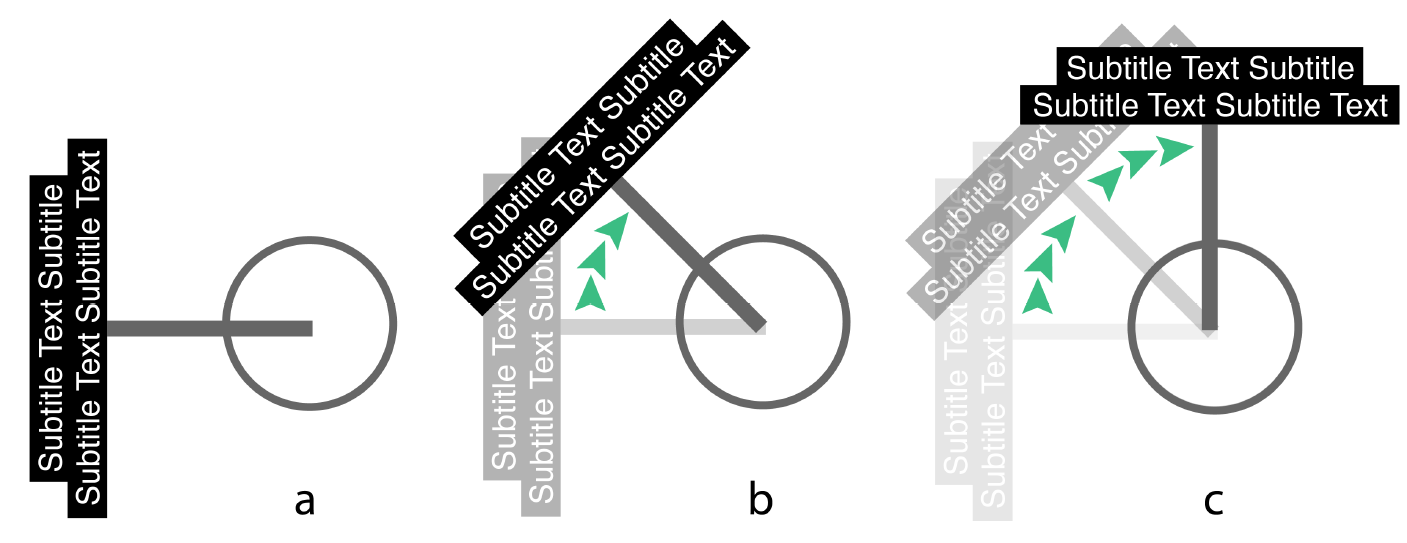
\includegraphics[width=0.7\textwidth]{img/video360/static-follow.png}
    \caption{Static-Follow: The sequence a, b, c demonstrates how as the user turns their head, the subtitles stay fixed to the centre of their field of view. Extracted from the work of Brown et al. (2017).}
    \label{fig:static_follow}
\end{figure}

\subsubsection{Lag-Follow}
\label{subsubsec:lag_follow}

The work of \cite{brown_subtitles_2017} defines the \emph{lag-follow}~(see Figure \ref{fig:lag_follow}) strategy to address the sickness related to the \emph{static-follow} strategy while still keeping the subtitles visible to the viewer. Similar to the \emph{static-follow} strategy, the subtitles appear in front of the viewer. It remains in such position~(relative to the environment) until the viewer's head rotates more than the 30º threshold. The subtitles then smoothly rotates to be in front of the viewer again. It is worth noticing that the subtitles can only move along the horizontal axis. The main objective of this strategy is to provide freedom of movement to the viewer without immediate reaction from subtitles. \cite{brown_subtitles_2017} say, however, that this strategy may cause the viewer to reread the subtitles, which is not desirable.

\begin{figure}[!ht]
    \centering
    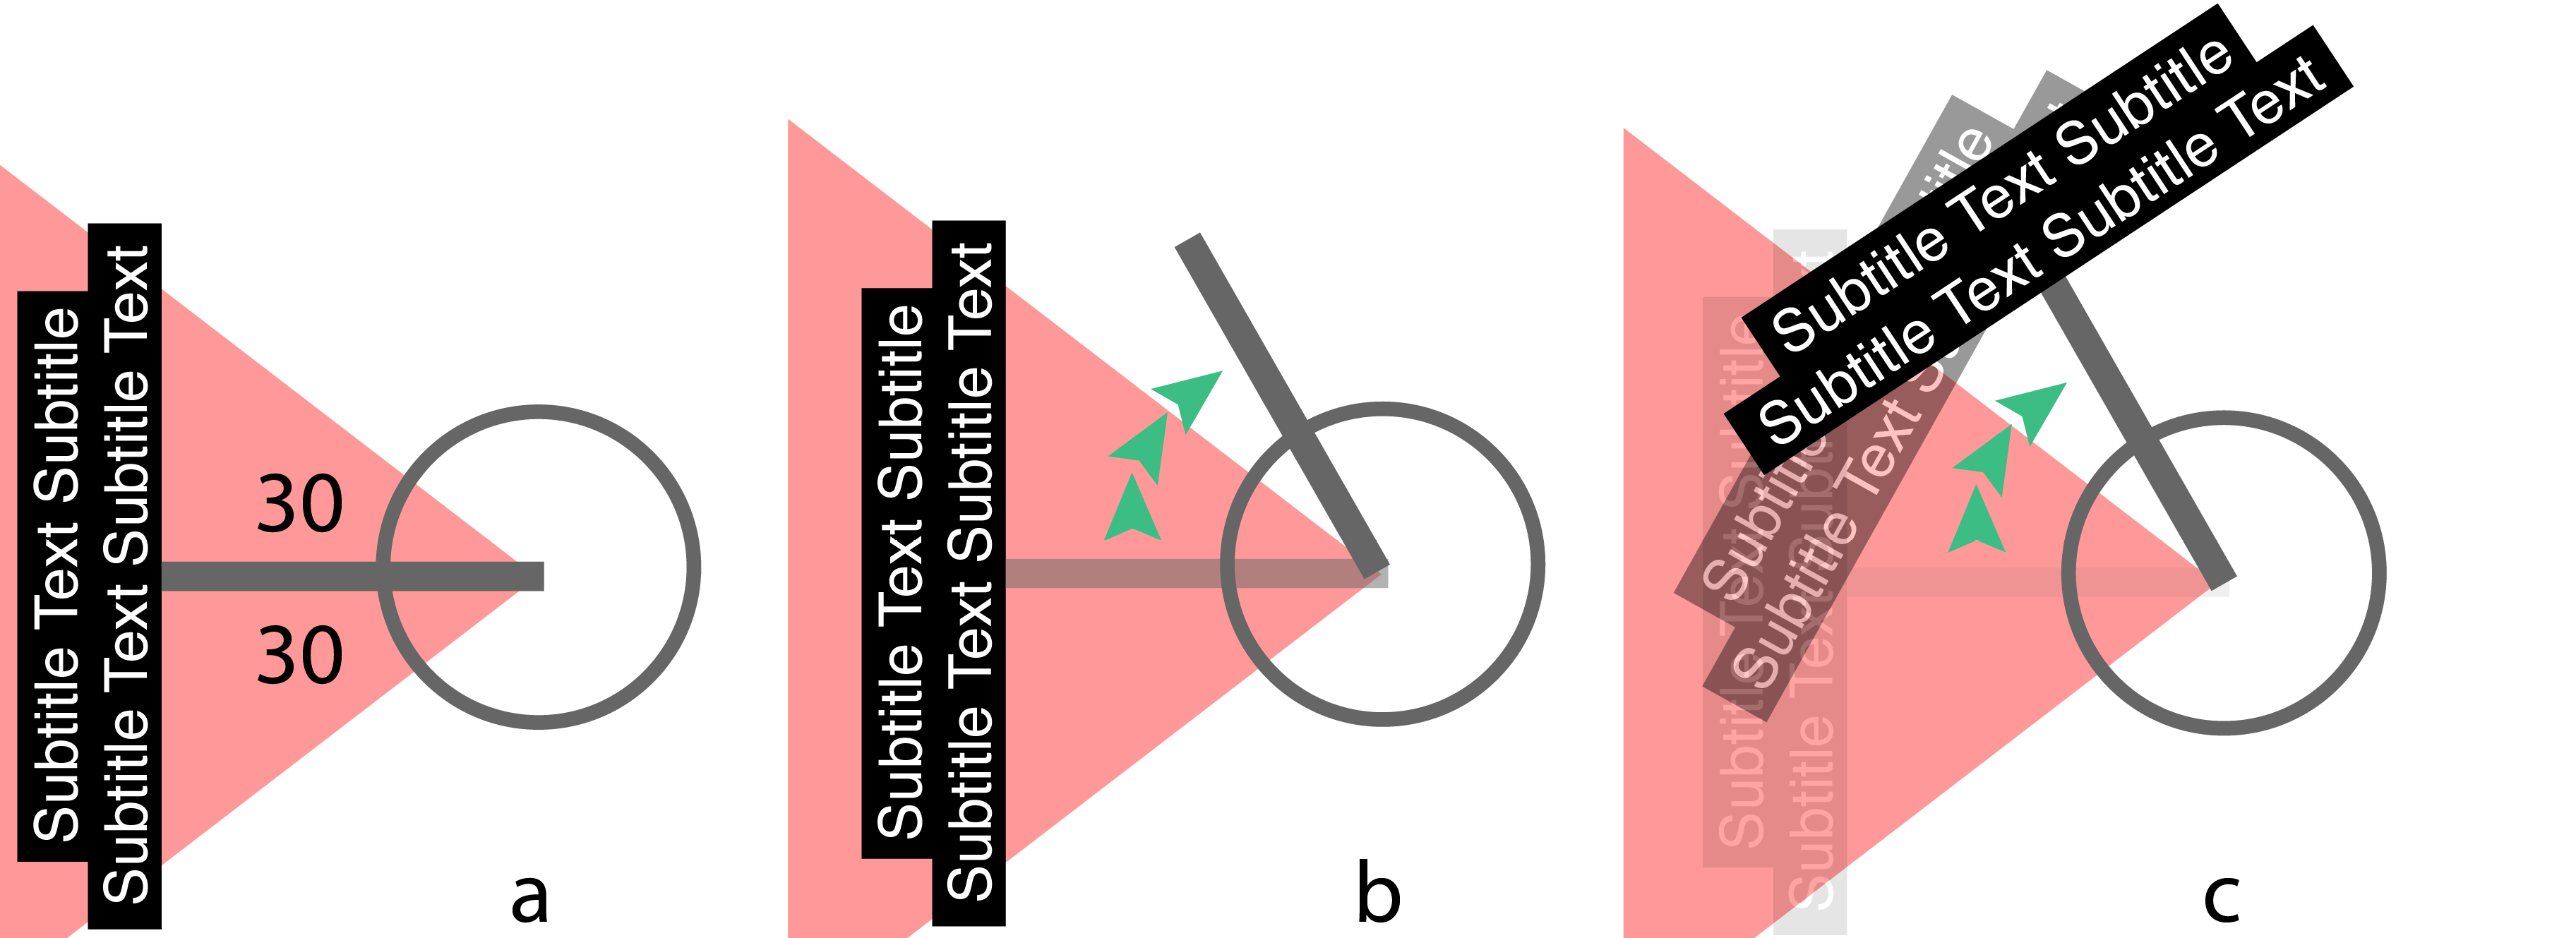
\includegraphics[width=0.7\textwidth]{img/video360/lag-follow.png}
    \caption{Lag-Follow: a. Small user head movements ($<30^{\circ}$) are ignored. b. But turning beyond this boundary c. The subtitles move smoothly to the center of the field-of-view. Extracted from the work of Brown et al. (2017).}
    \label{fig:lag_follow}
\end{figure}

The work of \cite{matos_dynamic_2018} describes a strategy that is basically the same of this one. It is called \emph{floating}, it starts in a position and floats into the viewer's field-of-view. Similar to what was described in Subsection \ref{subsubsec:static_follow}, the work of \cite{montagud_culture_2020} refers to this strategy with a different name (\emph{follow with lag}), but having the same definition.

\subsection{World-Referenced Subtitles}
\label{subsec:world_referenced}

In this category, the subtitles are positioned by taking the 360 environment as reference. 
As referenced in \cite{hughes_disruptive_2019}, this category of strategy leads to better results in comfort~\cite{rothe2018positioning}. \cite{rothe2018positioning}, as referenced in \cite{hughes_disruptive_2019}, also say that world-referenced subtitles conflict, in general, with the requirement that a user must always be able to read the subtitle text because it limitates the user's freedom of exploring the scene.
We have identified two strategies following this category: \emph{repeated subtitles} and \emph{appear subtitles}. These strategies are described in Subsections \ref{subsubsection:repeated_subtitles} and \ref{subsubsection:appear_subtitles}, respectively. 

\subsubsection{Repeated Subtitles}
\label{subsubsection:repeated_subtitles}

In this strategy, repeated subtitles are place around the user. These subtitles stay fixed in the environment and do not follow the user's head motion. Figure \ref{fig:120_subtitles} shows three repeated subtitles evenly spaced by angles of 120°. Such figure was extracted from the work of \cite{brown_subtitles_2017}. The authors argue that one of the main advantages of this strategy for subtitles positioning is that the subtitles could be ``burnt-in'' to the video using a video-editor. This strategy is referenced as \emph{120-degree} in the work of \cite{brown_subtitles_2017}, and as \emph{evenly spaced} in the work of \cite{montagud_culture_2020}. A caveat of this strategy, mentioned by \cite{brown_subtitles_2017}, is that it may cover important content located in unfortunate positions. 

The work of \cite{li_impacts_2018} uses this strategy to evaluate the impacts of subtitles in 360-degree video journalism. They do not evaluate the subtitles positioning itself, but the impact of the subtitles. The work of \cite{chen_film_2017} uses this strategy for positioning subtitles while investigating film language in society news using 360-degree videos of The New York Times. During their study, some participants found the \emph{repeated subtitles} strategy confusing as they thought, in some moments, that the subtitles in different positions had different text.

\begin{figure}[!ht]
    \centering
    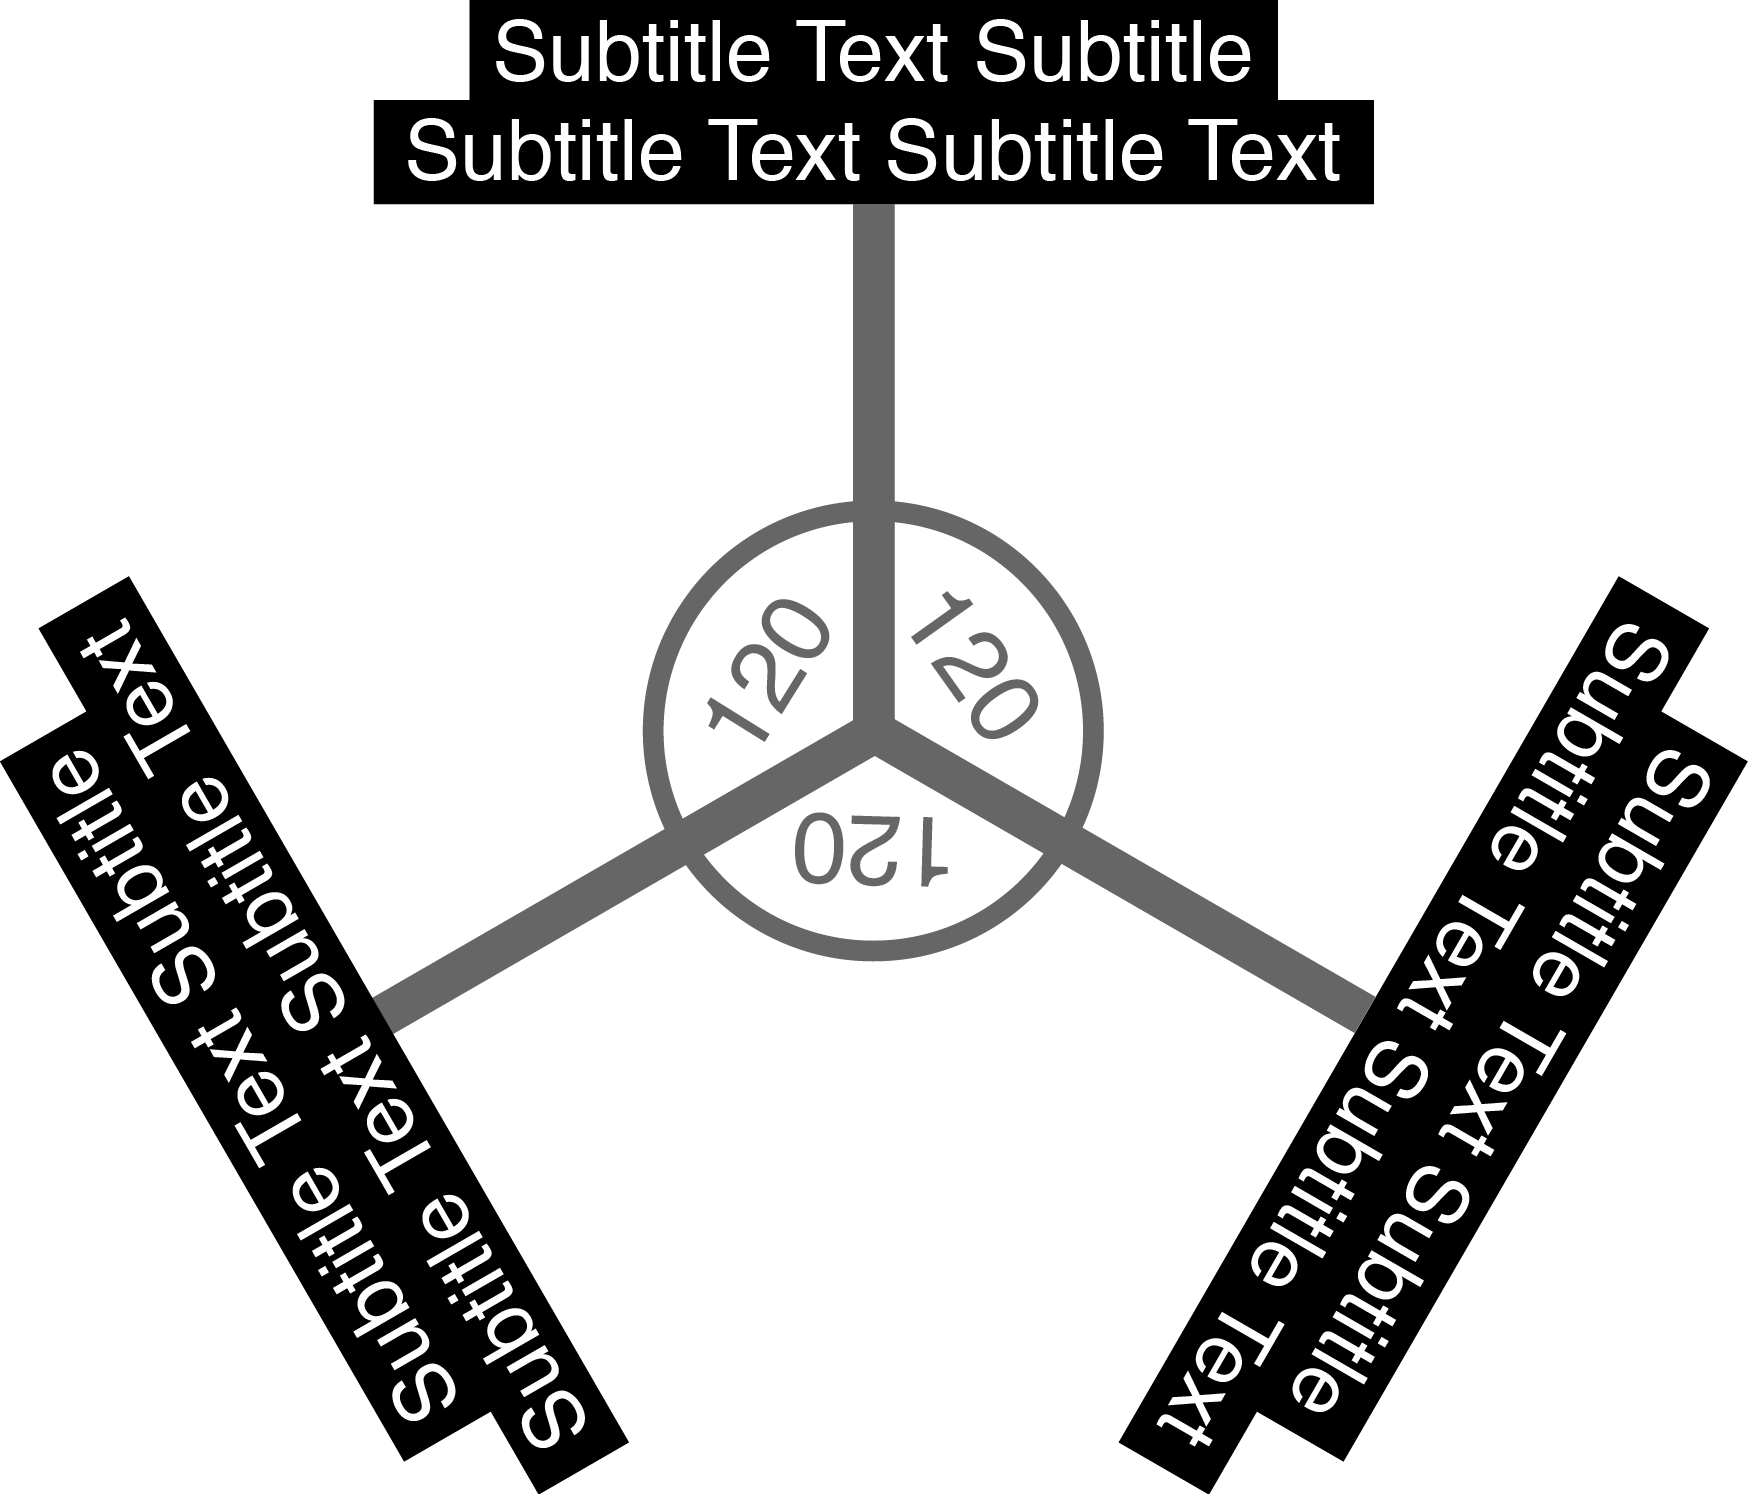
\includegraphics[width=0.35\textwidth]{img/video360/120_subtitles.png}
    \caption{Three repeated subtitles (having the same text) are located in the environment at 120° angles around the viewer. Extracted from the work of Brown et al. (2017).}
    \label{fig:120_subtitles}
\end{figure}


\subsubsection{Appear Subtitles}
\label{subsubsection:appear_subtitles}

\cite{brown_subtitles_2017} say that, based on feedback from a user whom was hard of hearing, they had the idea of creating a strategy in which the viewer can dismiss the subtitle after reading it. From that feedback, they designed the \emph{appear} strategy. As it is depicted in Figure \ref{fig:appear_subtitle}, the subtitles are placed at the centre of the user's field of view horizontally, 15º bellow eye-level. If the viewer moves their head, the subtitles remain static within the environment and do not follow their gaze. This strategy is also referenced as \emph{appear in front, then fixed} in the work of \cite{montagud_culture_2020}. A possible caveat of this strategy, mentioned by \cite{brown_subtitles_2017}, is that the subtitles may be positioned in spurious locations if the viewer is quickly moving their head.

\begin{figure}[!ht]
    \centering
    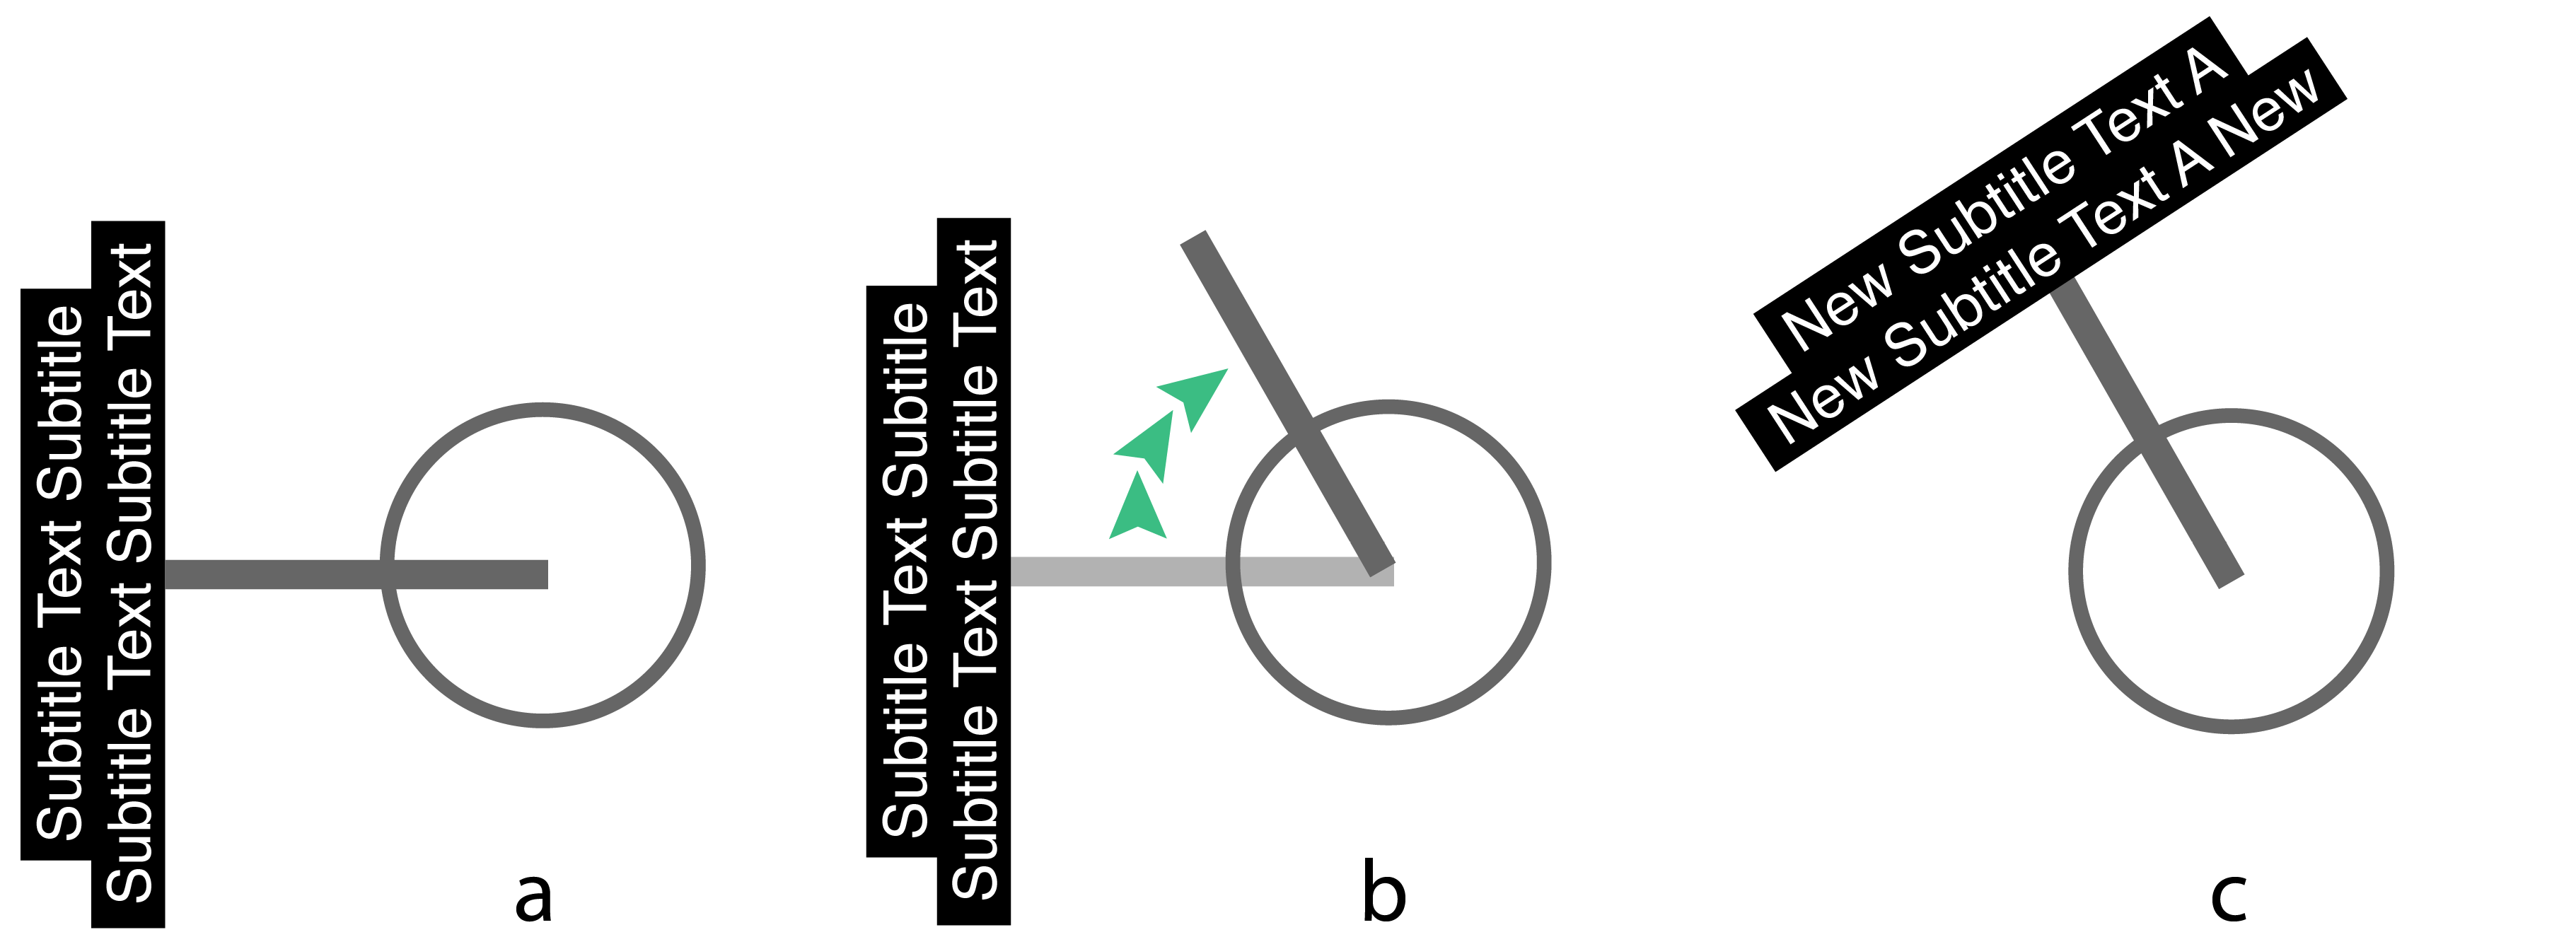
\includegraphics[width=0.7\textwidth]{img/video360/appear.png}
    \caption{Appear: a. A subtitle appears at the centre of the user's view. b. If the user moves before the subtitle is due to change, it will remain static in the environment. c. When a new subtitle is shown, it will appear at the centre of the user's view again. Extracted from the work of Brown et al. (2017).}
    \label{fig:appear_subtitle}
\end{figure}

\subsection{Dynamic Subtitles}
\label{subsection:dynamic_subtitles}

In this category, the position of subtitles dynamically changes and depends on the scene \cite{rothe_dynamic_2018}. As referring to annotations~(that could be subtitles), \cite{matos_dynamic_2018} say that there are cases where the point of interest is moving through the video, which requires a dynamic annotation that follows its movement. One strategy that we have identified in this category is the \emph{speaker-following subtitles} strategy, described in \ref{subsubsec:speaker_following}.

\subsubsection{Speaker-Following Subtitles}
\label{subsubsec:speaker_following}

In this strategy, the subtitles are placed close to the speaker~(see Figure \ref{fig:speaker_following}). Since the speakers may move during the video, this strategy fits in the \emph{dynamic subtitles} category. This strategy also helps in the issue of \emph{speaker identification}, as all persons in the room are visible in a 360-degree video~\cite{rothe_dynamic_2018}.  

\cite{rothe_dynamic_2018} compared \emph{speaker-following} subtitles with the \emph{static-follow} strategy regarding task workload, simulator sickness and presence. For evaluating each of these dimensions, the authors used, respectively, the following questionaires: NASA-TLX~\cite{nasa_hart1988development}; Simulator Sickness Questionaire~\cite{sickness_kennedy1993simulator}; and Presence Questionaire~\cite{presence_witmer1998measuring}. When asking which strategy the participants preferred, the authors received balanced answers. However, \emph{speaker-following} subtitles led to higher score of presence, less sickness and lower workload~\cite{rothe_dynamic_2018}.

\begin{figure}[!ht]
    \centering
    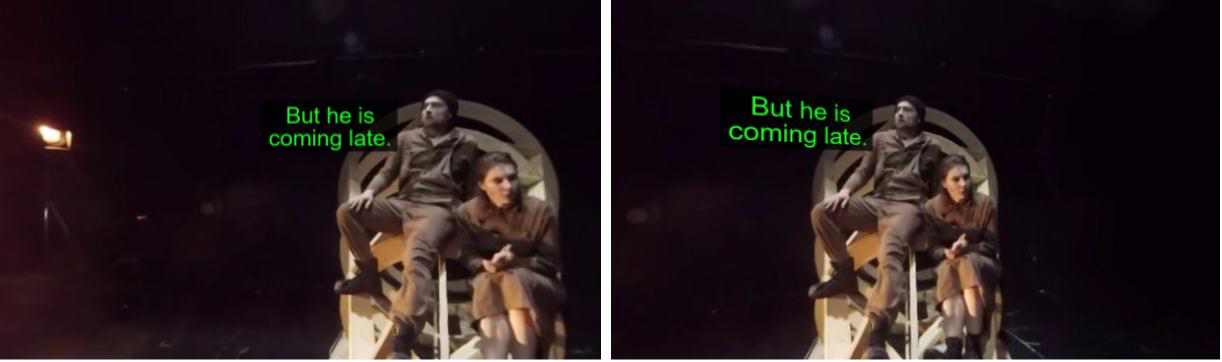
\includegraphics[width=0.95\textwidth]{img/video360/speaker-following.png}
    \caption{Speaker-following subtitles. Extracted from the work of Hughes et al. (2019).}
    \label{fig:speaker_following}
\end{figure}


Similar to the work of \cite{rothe_dynamic_2018}, we intend to position subtitles close to the speakers in the 360-video. The main difference of our work, however, is that we automatically detect the actors present in a 360-video and use their position for placing the subtitles according to an authoring model we propose. In our authoring model, we can also determine the direction that the user is looking at. We use that to position the subtitles as \emph{static-follow} when the actor speaking is not visible to the user. In this way, the disadvantage of \emph{speaker-following} subtitles being not always visible is suppressed.
\chapter{A Method For Video Face Clustering Method}
\label{chap:video_face_clustering}

This chapter describes the core of this dissertation, which is a method for \emph{Video Face Clustering}.
It consists of detecting and grouping faces from different video frames~(ideally from the same actors) extracted from a video file.
Figure \ref{fig:video_face_clustering} depicts this process, and each of its steps is described in the next paragraphs.

\begin{figure*}[!ht]
    \centering
    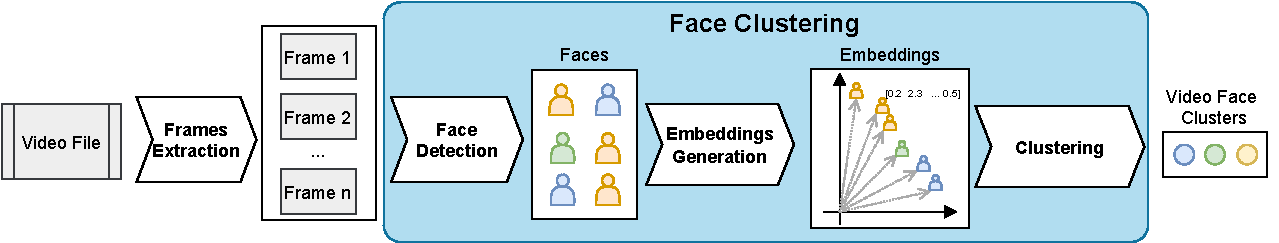
\includegraphics[width=\textwidth]{img/face_clustering/video_face_clustering.pdf}
    \caption{Video face clustering process.}
    \label{fig:video_face_clustering}
\end{figure*}


First, we perform \textit{Frames Extraction} by receiving a video file as input and extracting its frames according to a given frame rate. 
These frames are used as a set of images for the next step.

The \textit{Face Detection} step uses an object detection model for detecting faces in each of its images.
In general, any object detection model can identify which, among a known set of objects, are present in the image, and provides information about their positions.
In our case, objects are faces and, therefore, the face detection model is responsible for returning the bounding boxes of the faces present in the image, specified by the $x$ and $y$ axes coordinates of the upper-left corner and of the lower-right corner of the rectangle that establishes the visual limits that encapsulate each face. 
With these bounding boxes, we can isolate and extract the bounded images, obtaining a dataset composed of images of faces only.


The objective of the \textit{Embeddings Generation} step is to represent each face image as a vector in $\mathbb{R}^{n}$.
To achieve that, it processes each of the faces generated in the previous step through a CNN, generating embeddings. 
An embedding is a representation of the input in a lower-dimensional space.
Ideally, an embedding captures some semantics of the input, e.g. by placing semantically similar inputs close together in the embedding space.
At the end of this step, we have all faces represented as embeddings.

In the \textit{Clustering} step, we group embeddings and, consequently, faces that are close in the embedding space using a clustering algorithm. 
Clustering is the task of dividing a set of data points, embeddings in this case, into groups~(clusters) such that data points in a given group are similar to other data points in the same group and dissimilar to the data points in other groups.
The clustering process should produce a partition of the dataset, i.e., each generated cluster represents a specific person, and the union of all clusters covers the whole dataset. 
It is common for clustering algorithms to require the number of clusters in advance.
However, in the context of \emph{Video Face Clustering}, we do not know this number in advance, that is the number of actors in the video. 
For that reason, we have designed a strategy for automatically choosing an adequate number of clusters.
Section \ref{subsec:unknown_nclusters} describes this strategy.

\section{Iterative Strategy for Unknown Number of Clusters}
\label{subsec:unknown_nclusters}

In this Section, we define a strategy based on the \emph{Silhouette Score} ($s$) \cite{rousseeuw1987silhouettes} to choose an adequate clustering configuration.
The \emph{Silhouette Score}~\cite{rousseeuw1987silhouettes} corresponds to the mean of the \emph{Silhouette Coefficient} of all samples.
This coefficient ($S$) for each sample is 

\begin{equation}
\label{equation:Silh}
    S = \frac{b-a}{max(a,b)} 
\vspace{1em}
\end{equation}
%%
where $a$ is the mean distance from a sample to all other samples in the same cluster, and $b$ is the mean distance from a sample to all other samples in the closest cluster to that sample.
In this way, the best value is 1 and the worst is -1. Values close to 0 indicate overlapping clusters, whereas negative values usually indicate that a sample has been assigned to the wrong cluster since a different cluster is more similar.

With this strategy~(see Algorithm 1), we increase the number of clusters until the maximum \emph{Silhouette Score} decreases no more than $t$ times in a row or until it reaches the maximum number of clusters~(lines 5-18), which is the number of embeddings~($|e|$).
The \texttt{Clustering} procedure (line 7)
can be substituted by any clustering algorithm that requires the number of clusters in advance.
When the iteration stops, we return the clustering configuration with the highest \emph{Silhouette Score}.
Since this score requires at least two clusters, it would not be possible to compute it for a clustering configuration with only one cluster~(there are only faces of a single actor).
To overcome this problem, we start with 2 clusters consecutively increasing it as described above. Then, if the returned clustering configuration has a \emph{Silhouette Score} smaller than a threshold $\omega$, that probably indicates overlapping, we say that all faces belong to one single cluster~(lines 19-20). 

\begin{algorithm}
\small
\caption{Iteratively finding the best clustering configuration for unknown number of clusters.}\label{clustering_alg}
\begin{algorithmic}[1]
\Procedure{BlindClustering}{$e, t,\omega$}\
\State $n_K\gets 1$
\State $s_{max}\gets -1$
\State $t_{cur}\gets 0$ 

\While{$t_{cur} \leq t \And n_K < |e|$}
    \State $n_K\gets n_K+1$
    \State $K_{cur}\gets Clustering(e, n_K)$
    \State $s \gets SilhouetteScore(K_{cur})$
    \If{$s < s_{max}$}
        \State $t_{cur}\gets t_{cur}+1$
    \Else
        \State $K\gets K_{cur}$
        \State $t_{cur}\gets 0$
        
        \If{$s > s_{max}$}
            \State $s_{max} \gets s$
        \EndIf
    \EndIf
\EndWhile
\If{$s_{max} < \omega$}
    \State $K\gets OneCluster(e)$
\EndIf
\State \textbf{return} $K$
\EndProcedure
\end{algorithmic}
\end{algorithm}


By the end of this process, we expect to have the spatiotemporal localization of the actors present in a video file.
Figure \ref{fig:timeline} shows an example of the results achieved by our \emph{Video Face Clustering} method. It contains a timeline of a video with lines coloring the segments that each actor appears in.

\begin{figure}[!ht]
    \centering
    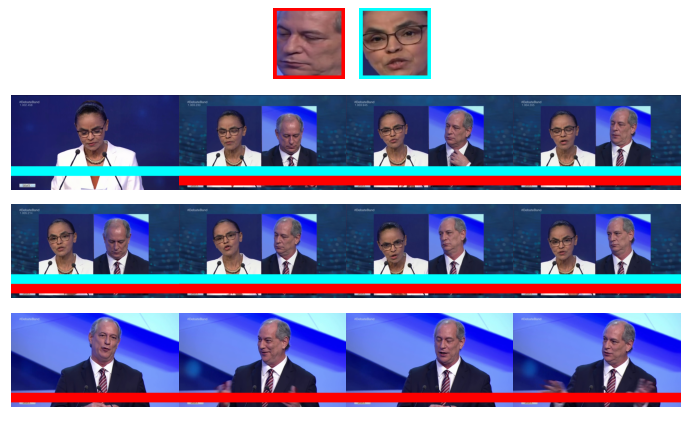
\includegraphics[width=0.65\linewidth]{img/face_clustering/example_localization.png}
    \caption{Example of spatiotemporal localization.}
    \label{fig:timeline}
\end{figure}

The following three chapters describe the applications we investigate in this dissertation. 
These three applications propose novel approaches for tasks in video using spatiotemporal localization of actors through \emph{Video Face Clustering}.


\newpage
\chapter{Cluster-Matching-Based Method For Video Face Recognition}
\label{chap:face_recognition}

In this chapter, we describe the first application we investigated using the \emph{Video Face Clustering} method.
%%
We propose a cluster-matching-based approach for video face recognition where \emph{face clustering} is used to group faces in both the face dataset and in the target video~(video face clustering).
%%
Consequently, classes do not have to be previously known, and the effort spent with annotations is significantly reduced --- as it is done over clusters instead of single images.
%%
Face recognition becomes a task of comparing clusters from the dataset with the ones extracted from images or video sources.
%%
Therefore, our approach is easily scalable.

This chapter is structured as follows. 
%%
In Section \ref{sec:recognition_dataset}, we describe the dataset we produced to perform experiments. 
%%
In Section \ref{sec:recognition_method}, we detail our proposed method, followed by two sections with experiments: 
%%
Section \ref{sec:recognition_clustering_validation}, regarding the clustering methods we use, and 
%%
Section \ref{sec:recognition_matching_validation}, with the experiments with our matching heuristic.
%%
Section \ref{sec:recognition_video_evaluation} is devoted to the overall evaluation of our method and, finally, 
%%
in Section \ref{sec:recognition_discussion}, we conclude this chapter by discussing our results.

\section{Dataset}
\label{sec:recognition_dataset}
Our dataset was collected using the information provided by the Brazilian Chamber of Deputies\footnote{\url{https://www.camara.leg.br/}} for the 55th legislature, which was in session from February 1st, 2015 through January 31st, 2019.
%%
In total, 623 different deputies participated during some period in the 55th legislature, but we collected only 513 deputies from this set.

For each of the 513 deputies, we collected images in which he/she was present using Google images.
%%
The resulting dataset has a total of 9,003 images, with a mean of ~17.55 images per deputy and a standard deviation of ~6.91. 
%%
The maximum and minimum number of images per deputy are respectively 32 and 2.
%%
We have randomly selected one image of each deputy for validation and the rest for training.
%%
Thus, our dataset is divided into two: the training set, with 8,490 images, and the validation set, with 513 images.  

Besides, we created another set containing images of people who are not present in the deputies set.
%%
For that, we randomly selected 513 images from the \emph{Labeled Faces in the Wild}~(LFW)~\cite{LFWTech} dataset, that contains more than 13,000 images of faces collected from the web,
%%
and defined this subset of LFW as our \emph{Non-registered people} set.

\section{Proposed Method}
\label{sec:recognition_method}

Our method intends to recognize people in video using CNNs and clustering algorithms.
%%
Figure \ref{fig:cluster_matching} shows our proposed approach.

\begin{figure*}[!ht]
    \centering
    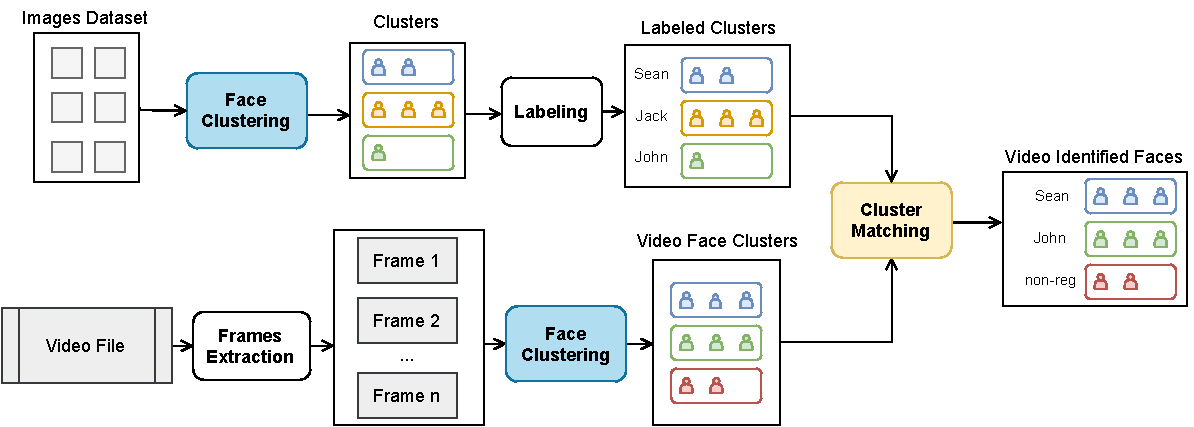
\includegraphics[width=\textwidth]{img/face_recognition/cluster_matching_process.pdf}
    \caption{Cluster-Matching based Method for Video Face Recognition.}
    \label{fig:cluster_matching}
\end{figure*}

In our approach we use \emph{Face Clustering} in an images dataset and in the referenced video. Then, the clusters of the images dataset are labeled. 
%%
In the \textit{Labeling} step, we assign labels~(identities) to represent the clusters.
%%
A label can be anything that represents the faces present in the cluster, e.g. a name or an id number. 
%%
Using this pipeline, instead of having to label every single face for constructing a labeled dataset, it is only necessary to label each generated cluster.
%%
Consequently, all the faces present in a cluster are assigned to the same label. 
%%
Hence, the complexity of labeling becomes a function dependent on the number of clusters, which is at most as great as the number of individuals.
%%
At the end of this step, we have a dataset of \emph{Labeled Clusters}.


Next, we perform \emph{Cluster Matching} where the clusters from the image dataset and from the video are matched using a heuristic based on clusters distance.

The \textit{Cluster Matching} step receives the set of clusters from the video and the set of labeled clusters, which is used as a reference for recognizing the clusters (and consequently the faces) in the video.
%%
%%
We designed a method based on cluster distance for performing this recognition.
%%
We compare each candidate cluster in the video with each of the labeled clusters in the reference dataset, using what we call a \emph{cluster embedding}. This \emph{cluster embedding} is computed for both the candidate cluster in the video and the reference cluster in the labeled dataset.
%%
The \emph{cluster embedding} maps each cluster to a vector in the embedding space of the face embeddings.
%%
In the experiments, we evaluate two ways of obtaining a \emph{cluster embedding}.

Let $q$ denote the \emph{cluster embedding} of the query cluster, where $q~\in~\mathbb{R}^{n}$, in which $n$ is the dimension of the embedding space.
%
Let $K$ denote the set of labeled clusters. For each $k~\in~K$, let $c_k$ denote the \emph{cluster embedding} of $k$. 
%
We compute a similarity function of $q$ and each $c_k$ for $k~\in~K$. 
%%
This similarity function is based on the Root Mean Square Error~(RMSE) function, which is largely used for computing embeddings distances in machine learning techniques.\footnote{https://www.sciencedirect.com/topics/engineering/root-mean-square-error}
%%
We decided to use the inverse of the RMSE since we want to return larger values for clusters that are closer to $q$, to be able to use these values to compute a probabilistic distribution:

\begin{equation}
\label{equation:similarity_raw}
    s_{q,k} = \frac{1}{\sqrt{\frac{1}{n}\sum_{i=0}^{n}{(q_i-c_{k,i})^2}}}
\end{equation}

Since we are not interested in clusters that too distant from $q$, we define $\overline{s}_{q,k}$ that considers only the $\alpha$ largest $s_q$ values. The $\alpha$ value is a parameter that we further evaluate in this work. 
Thus, our similarity function becomes

\begin{equation}
\label{equation:similarity}
    \overline{s}_{q,k} = \begin{cases}s_{q,k} & \text{if}~s_{q,k}~\in max_{\alpha(s_q)}\\0 & \text{otherwise}\end{cases}
\end{equation}

Given the similarity~$\overline{s}_{q,k}$, we compute the probability of $q$ being a match with each labeled cluster using the \emph{softmax} function.
%%
This function takes as input a vector of real numbers and normalizes it into a probability distribution consisting of probabilities proportional to the exponential of the input numbers. 
It is defined as

\begin{equation}
\label{equation:probability}
    p_{q,k} = \frac{e^{\overline{s}_{q,k}}}{\sum_{j~\in~K}{e^{\overline{s}_{q,j}}}}
\end{equation}

Finally, we define the function $\sigma$ that, given a \emph{cluster embedding} query $q$, returns the cluster in the labeled clusters whose \emph{cluster embedding} is more likely to have a match with the query if it has a probability greater than $0.5$. Otherwise, the query is assigned as being a match with none of the clusters ($\text{\o}$ is given as result). The $\sigma$ function is defined as follows.

\begin{equation}
\label{equation:sigma}
    \sigma{(q)} = \begin{cases}argmax(p_q) & if~~~p_{q,argmax(p_q)}~>~0.5\\\text{\o} & otherwise\end{cases}
\end{equation}

The $argmax$ function applied over $p_q$ returns the cluster $k$ whose probability of $q$ being a match with it is the greatest. 
%%
We observed that when a cluster has faces that belong to a person present in the labeled clusters, the probability tends to be higher for one single labeled cluster.
%%
However, when the person is not in any of the labeled clusters, the probability tends to be more distributed among different labeled clusters.
%%
For that reason, when none of the labeled clusters has a probability greater than $0.5$, we say that the query cluster does not match any of the labeled clusters.
%%
Hence, the person in the video represented by the query cluster is not present in the labeled clusters.

\section{Faces Clustering Validation}
\label{sec:recognition_clustering_validation}

In this section, we evaluate the quality of the clustering generated in the macro-step \emph{Face Clustering}.
%%
In the \emph{Face Detection} step, we use MTCNN~\cite{mtcnn} (Multitask
Cascaded Convolutional Networks) which is widely used for the face detection task~\cite{mtcnn1, mtcnn3}.
%%
We used the  \emph{mtcnn} Python library for its implementation\footnote{\url{https://pypi.org/project/mtcnn/}} and resized each face detected to 224x224.
%%
We tested three different CNNs for the \emph{Embeddings Generation} step in association with three different clustering algorithms for the \emph{Clustering} step.
%%
For that, we evaluated each pair of \emph{CNN x ClusteringAlg} through the quality of the clusters they generated. 
%%
To experiment, we used the training set with 8490 deputy images.

In what follows, we describe the algorithms used for the experiments, the metrics used to evaluate and the results we obtained.

\subsection{Embeddings Generation}
%\label{subsec:exp_setup}

For this step, we have three candidate CNNs that were previously trained on the VGGFace2 dataset~\cite{cao2018vggface2}. 
%%
The VGGFace2 dataset contains $3.31$ million images of $9131$ subjects and has large variations in pose, age, illumination, ethnicity, and profession.
%%
The three candidate CNNs used are VGG-16~\cite{vgg16}, ResNet-50~\cite{resnet} and SE-ResNet-50~\cite{senet}~(SeNet-50 for short). VGG-16 generates embeddings in the $\mathbb{R}^{512}$  feature space, while ResNet-50 and SeNet-50 generate embeddings in the $\mathbb{R}^{2048}$ feature space. 


\subsection{Clustering Algorithms}
%\label{subsec:clustering_algs}
%%
For this step, we selected the following clustering algorithms as candidates: K-Means~(KM)~\cite{lloyd1982least}, Affinity Propagation~(AP)~\cite{frey2007clustering}, and Agglomerative Clustering~(AC)~\cite{ward1963hierarchical}. Each of these algorithms is briefly explained next.

K-Means~\cite{lloyd1982least} is one of the most widely used unsupervised machine learning algorithms. 
%%
To process the data to be clustered, the K-Means algorithm begins with a randomly selected group of $K$ centroids, which are updated iteratively to optimize the distance of the data points to the closest centroid.
The algorithm stops when either the centroids have stabilized or the maximum number of iterations has been reached.

The Affinity Propagation algorithm~\cite{frey2007clustering}, in contrast with other clustering methods, does not require the number of clusters to be previously specified.
%%
In this algorithm, each data point sends messages to the other points informing them of their relative attractiveness to the sender. 
%%
Those targets then reply to the senders informing their availability to associate with them, considering the attractiveness of all the messages it received.
%%
The senders then reply to the targets informing the target's updated relative attractiveness.
%%
This process continues until a consensus is established.
%%
When the sender data point is associated with one of its targets, that target becomes the point's exemplar.
%%
The points with the same exemplar are assigned to the same cluster.

The Agglomerative Clustering algorithm recursively merges the pair of clusters that minimally increase a given linkage distance.
%%
The linkage criteria specify the distance to use between two sets of data points.
%%
The Agglomerative Clustering algorithm~\cite{ward1963hierarchical} merges pairs of clusters that minimize the linkage criteria.
%%
In this work, we chose the \emph{Ward} criteria~\cite{ward1963hierarchical}, which minimizes the variance of the clusters being merged.
%%
By using this method, at each step, the algorithm finds the pair of clusters that leads to a minimum increase in total within-cluster variance after merging.
%%
This increase is measured by a weighted squared distance between cluster centers.
%%
In the first step, each data point is a cluster.
%%
The clusters are merged following the criteria until the number of clusters $K$ is reached.

Different from the Affinity Propagation algorithm, K-Means and Agglomerative Clustering require the number of clusters in advance. For this case, we used 513~(number of deputies in the \emph{train set}).
%%
However, when the number of cluster is not known, a strategy for defining it is required for these two algorithms.

\subsubsection{Iterative Strategy for Unknown Number of Clusters}
\label{subsec:unknown_nclusters}

We use a strategy based on the \emph{Silhouette Score} ($s$) \cite{rousseeuw1987silhouettes} to choose the best clustering configuration.

The \emph{Silhouette Score}~\cite{rousseeuw1987silhouettes} corresponds to the mean of the \emph{Silhouette Coefficient} of all samples.
%%
This coefficient ($S$) for each sample is 
\begin{equation}
\label{equation:Silh}
    S = \frac{b-a}{max(a,b)} 
\end{equation}
%%
where $a$ is the mean distance from a sample to all other samples in the same cluster, and $b$ is the mean distance from a sample to all other samples in the closest cluster to that sample.
%%
In this way, the best value is 1 and the worst is -1. Values close to 0 indicate overlapping clusters, whereas negative values usually indicate that a sample has been assigned to the wrong cluster since a different cluster is more similar.

With this strategy~(see Algorithm 1), we increase the number of clusters until the maximum \emph{Silhouette Score} decreases no more than $t$ times in a row or until it reaches the maximum number of clusters~(lines 5-18)
, which is the number of embeddings~($|e|$).
%%
The \texttt{Clustering} procedure (line 7)
can be substituted by any clustering algorithm that requires the number of clusters in advance.
%%
When the iteration stops, we return the clustering configuration with the highest \emph{Silhouette Score}.
%%
Since this score requires at least two clusters, it would not be possible to compute it for a clustering configuration with only one cluster~(there are only faces of a single person).
%%
To overcome this problem, we start with 2 clusters consecutively increasing it as described above. Then, if the returned clustering configuration has a \emph{Silhouette Score} smaller than a threshold $\omega$, that probably indicates overlapping, we say that all faces belong to one single cluster~(lines 19-20). 

\begin{algorithm}
\small
\caption{Iteratively finding the best clustering configuration for unknown number of clusters.}\label{clustering_alg}
\begin{algorithmic}[1]
\Procedure{BlindClustering}{$e, t,\omega$}\
\State $n_K\gets 1$
\State $s_{max}\gets -1$
\State $t_{cur}\gets 0$ 

\While{$t_{cur} \leq t \And n_K < |e|$}
    \State $n_K\gets n_K+1$
    \State $K_{cur}\gets Clustering(e, n_K)$
    \State $s \gets SilhouetteScore(K_{cur})$
    \If{$s < s_{max}$}
        \State $t_{cur}\gets t_{cur}+1$
    \Else
        \State $K\gets K_{cur}$
        \State $t_{cur}\gets 0$
        
        \If{$s > s_{max}$}
            \State $s_{max} \gets s$
        \EndIf
    \EndIf
\EndWhile
\If{$s_{max} < \omega$}
    \State $K\gets OneCluster(e)$
\EndIf
\State \textbf{return} $K$
\EndProcedure
\end{algorithmic}
\end{algorithm}

\subsection{Metrics}
%\label{sec:metrics}

We evaluate the models using the V-Measure~\cite{vmeasure}, which is an entropy-based measure that computes how successfully the criteria of homogeneity and completeness have been satisfied. This metric is extensively used for comparing clustering solutions and has been used in different domain fields such as biology~\cite{bio1}, computational linguistics~\cite{nlp1}, and document engineering~\cite{doceng}.


The V-Measure is a harmonic mean of homogeneity and completeness scores, similar to how precision and recall are frequently combined into F-measure~\cite{van1979information}. It assumes a dataset comprising $N$ data points, and a set of classes, $C = \{c_i|i = 1,..., n\}$ and a set of clusters, $K = \{k_i|i = 1,...,m\}$. They also assume $A$ as a matrix produced by the clustering algorithm representing the clustering solution, such that $A = \{a_{ij}\}$ where $a_{ij}$ is the number of data points that are members of class $c_i$ and elements of cluster $k_j$.

The homogeneity is perfect when a clustering algorithm assigns only those data points that are members of a single class to a single cluster, so that the entropy is zero in each cluster.
%%

In this way, the homogeneity score determines how close a given clustering is to this ideal by examining the conditional entropy of the class distribution given the proposed clustering. 
%%
Therefore, when the clustering is perfectly homogeneous, such a value, $H(C|K) = 0$. 
 
On the other hand, when the clustering is not perfect according to this criterion, this value is proportional to the size of the dataset and the classes.
%%
For this reason, the authors normalize this value by the maximum reduction in entropy the clustering information could provide, specifically, $H(C)$.
%%
$H(C|K)$ has its maximal value when it is equal to $H(C)$ and provides no new information.
%%

Finally, to address to the convention of $1$ being desirable and $0$ undesirable, the authors define homogeneity as:

\begin{equation}
\label{equation:homo}
    h = \begin{cases} 1 & \text{if}\ H(C|K) = 0 \\1-\frac{H(C|K)}{H(C)} & \text{otherwise}\end{cases}
\end{equation}

where

\begin{equation}
    H(C|K) =  -\sum_{k=1}^{|K|}{\sum_{c=1}^{|C|}{\frac{a_{ck}}{N}log\frac{a_{ck}}{\sum_{c=1}^{|C|}{a_{ck}}}}}
\end{equation}

\begin{equation}
    H(C) = -\sum_{c=1}^{|C|}{  \frac{\sum_{k=1}^{|K|}a_{ck}}{n}log \frac{\sum_{k=1}^{|K|}a_{ck}}{n} }
\end{equation}

Completeness is symmetrical with respect to homogeneity, and it is perfect when a clustering assigns all data points that are members of the same class to a single cluster. 
%%
For computing such a score, the authors examine the distribution of cluster assignments within each class.
%%
Completeness is defined as 

\begin{equation}
\label{equation:completeness}
    c = \begin{cases} 1 & \text{if}\ H(K|C) = 0 \\1-\frac{H(K|C)}{H(K)} & \text{otherwise}\end{cases}
\end{equation}

where

\begin{equation}
    H(K|C) =  -\sum_{c=1}^{|C|}{\sum_{k=1}^{|K|}{\frac{a_{ck}}{N}log\frac{a_{ck}}{\sum_{k=1}^{|K|}{a_{ck}}}}}
\end{equation}
\vspace{1em}
\begin{equation}
    H(K) = -\sum_{k=1}^{|K|}{  \frac{\sum_{c=1}^{|C|}a_{ck}}{n}log \frac{\sum_{c=1}^{|C|}a_{ck}}{n} }
\end{equation}

Finally, by using Equation \ref{equation:homo} and Equation \ref{equation:completeness}, V-measure is defined as 
\begin{equation}
    V_{\beta} = (1+\beta)\frac{h\cdot c}{\beta\cdot{h+c}}
\end{equation}

The parameter $\beta$ is used to calibrate the relative importance of homogeneity and completeness when computing the V-measure. If $\beta$ is greater than 1, the completeness is more important for the V-measure, whereas 
%%
if $\beta$ is less than 1, homogeneity is more important for the V-measure. 
%%
In this work, we use $\beta = 1$, so that completeness and homogeneity contribute equally to the V-measure.

\subsection{Results}
\label{subsec:results}

Table \ref{tab:results_clustering} shows the homogeneity, completeness, and V-Measure for each combination of CNN and clustering algorithm.

From Table \ref{tab:results_clustering}, one can conclude that the best combination of CNN and clustering algorithm was SeNet-50 with Agglomerative Clustering.
%%
For this reason, we decided to use SeNet-50 for the \emph{Embeddings Generation} step and the Agglomerative Clustering algorithm for the \emph{Clustering} step.
%%
As a result, each face on the dataset is represented as an embedding in the $\mathbb{R}^{2048}$ produced by SeNet-50.

\begin{table}[!ht]
\centering
\small
\caption{Results of the evaluation of the clusters created by each combination of CNN and clustering algorithms.}
\begin{tabular}{@{}ccccc@{}}
\toprule
\textbf{CNN} & \textbf{Clustering} & \textbf{$h$} & \textbf{$c$} & \textbf{$V_1$} \\ \midrule
                  & KM                  & 0.9665                     & 0.9675                      & 0.9670             \\
ResNet-50         & AP                  & 0.0000                     & 1.0000                      & 0.0000             \\
                  & AC                  & 0.9821                     & 0.9798                      & 0.9810             \\ \midrule
                  & KM                  & 0.9725                     & 0.9726                      & 0.9725             \\
SeNet-50          & AP                  & 0.9859                     & 0.9558                      & 0.9706             \\
                  & \textbf{AC}         & \textbf{0.9862}            & \textbf{0.9833}             & \textbf{0.9847}    \\ \midrule
                  & KM                  & 0.8340                     & 0.8415                      & 0.8378             \\
VGG-16            & AP                  & 0.0000                     & 1.0000                      & 0.0000             \\
                  & AC                  & 0.8899                     & 0.8929                      & 0.8914             \\
\end{tabular}
\label{tab:results_clustering}
\end{table}

One can observe that the Affinity Propagation algorithm had a V-measure of $0$ when used with ResNet-50 and VGG-16. 
%%
This happens because, in both cases, the algorithm assigned all the data points~(face embeddings in this context) to one single cluster. 
%%
Consequently, those combinations had a homogeneity score of $0$ because there was no information gain after clustering--and completeness of 1 because data points of the same class were not scattered in different clusters.
%%
With such a combination, the V-measure, which is a harmonic mean of the homogeneity and completeness, has a value of $0$.


\section{Cluster-Matching Validation}
\label{sec:recognition_matching_validation}

Based on the results of the experiment described in Section \ref{sec:recognition_clustering_validation}, we developed another experiment in order to choose the best $\alpha$ value in Equation \ref{equation:similarity} and the best method for computing the \emph{cluster embedding} for the clusters.

As the best combination for clustering was SeNet-50 with the Agglomerative Clustering algorithm, this experiment uses the embeddings and labeled clusters generated by it.
%%
Hence, the labeled clusters are the set of faces from the 8490 deputy images with their respective embeddings and labels.
%%
Each cluster was labeled with the name of the deputy whose face is more frequent in it.

For testing, we used the \emph{Validation set}~($V$) consisting of 513 deputy images and the \emph{Non-registered people set}~($U$) also consisting of 513 images.
%%
We used these images as if they were the clusters from a video file, each cluster having a single sample.
%%
In this way, we have a more heterogeneous set for performing this experiment as if we had used a small set of video files.

We evaluate two methods for computing a \emph{cluster embedding} for the labeled clusters: \emph{cluster centroid} and \emph{sample with best silhouette coefficient}. A cluster centroid denotes the mean of the elements in a cluster.
%%
It is calculated the mean of all elements in a cluster for each axis in the embedding space. The second method uses the embedding of the sample whose silhouette coefficient is the highest.
%%
This coefficient is calculated using the mean intra-cluster distance and the mean nearest-cluster distance for each sample~(detailed in Subsection \ref{subsec:unknown_nclusters}).

\subsection{Metrics}

We evaluate the two methods for computing the \emph{cluster embedding} by assessing how well the cluster matching recognizes registered people and correctly tells when a person is not registered.
%%
A non-registered person should not have a match with any of the labeled clusters.

Let $\lambda(q)$ be the most frequent label of a cluster $q$, $|V|$ the size of the \emph{Validation set} and $|U|$ the size of the \emph{Non-registered people set}.
%%
Although $\lambda$ represents the label of a cluster in general, we also define $\Lambda$ as being the set of all the face labels present in a cluster.
%%
Let us also assume true as $1$ and false as $0$.
%%
To perform the evaluation, we compute the following four metrics:

\vspace{2em}
\noindent\begin{minipage}[c]{0.45\linewidth}
    \begin{equation}
    \small
    m_1 = \sum_{v~\in~V}{\frac{\sigma(v)\ne\text{\o}}{|V|}}
    \end{equation}
\end{minipage}
\hfill
\begin{minipage}[c]{0.45\linewidth}
    \begin{equation}
    \small
    m_2 = \sum_{v~\in~V}{\frac{\lambda(v) = \lambda(\sigma(v))}{|V|}}    
    \end{equation}
\end{minipage}

\vspace{1em}

\noindent\begin{minipage}[c]{0.45\linewidth}
    \begin{equation}
    \small
    m_3 = \sum_{v~\in~V}{\frac{\lambda(v)~\in~\Lambda(\sigma(v))}{|V|}} 
    \end{equation}
\end{minipage}
\hfill
\begin{minipage}[c]{0.45\linewidth}
    \begin{equation}
    \small
    m_4 = \sum_{u~\in~U}{\frac{\sigma(u)=\text{\o}}{|U|}}
    \end{equation}
\end{minipage}
\vspace{2em}

Where $m_1$ denotes the percentage of clusters from $V$ matched with any cluster, $m2$ the percentage of clusters from $V$ matched with a cluster with the same label, $m3$ the percentage of clusters from $V$ matched with a cluster in which the label is present, and $m4$ that denotes the percentage of clusters from $U$ that have not matched with any cluster.

\subsection{Results}

In this subsection we show the results for each of the methods for generating the \emph{cluster embeddings} in the \emph{cluster matching} step.
%%
For each of the methods, we tested different $\alpha$ values in Equation \ref{equation:similarity}.

Table \ref{tab:results_centroid} shows the results obtained using the cluster centroids as \emph{cluster embeddings}.
%%
It can be seen that with the higher the $\alpha$ value is, the lower is the percentage of registered faces assigned to the correct labeled cluster.
%%
On the other hand, the percentage of non-registered faces assigned to none of the labeled clusters increases with the $\alpha$ value.
%%
One can see that with $\alpha = 5$, we have a balance between assigning people to the correct cluster and being able to tell when a person is not in the labeled clusters.

\begin{table}[!ht]
\centering
\small
\caption{Results obtained using cluster centroids as \emph{cluster embeddings}}
\label{tab:results_centroid}
\begin{tabular}{ccccc}
\hline
\textbf{$\alpha$} & \textbf{m1} & \textbf{m2} & \textbf{m3} & \textbf{m4} \\ \hline
2 & 100.000\% & 94.932\% & 98.246\% & 0.000\% \\
3 & 97.076\% & 94.152\% & 96.881\% & 94.542\% \\
4 & 95.517\% & 93.177\% & 95.322\% & 98.635\% \\
\textbf{5} & \textbf{94.542}\% & \textbf{92.398}\% & \textbf{94.347}\% & \textbf{99.220}\% \\
6 & 93.567\% & 91.813\% & 93.372\% & 99.610\% \\
7 & 92.788\% & 91.228\% & 92.593\% & 99.805\% \\
8 & 91.813\% & 90.643\% & 91.618\% & 99.805\% \\
9 & 90.448\% & 89.279\% & 90.253\% & 99.805\% \\
10 & 89.474\% & 88.304\% & 89.279\% & 99.805\%
\end{tabular}
\end{table}

Table \ref{tab:results_silhouette} shows the results obtained using the sample with the highest silhouette coefficient as the \emph{cluster embedding} for each of the labeled clusters.
%%
One can observe that the $\alpha$ value correlates with the percentage values similar to the one observed in Table \ref{tab:results_centroid}.
%%
By using the silhouette coefficient for choosing the \emph{cluster centroids}, we have an algorithm more capable of determining when a person is not registered, achieving a percentage of $100\%$ when $\alpha>5$.
%%
However, when using this approach, the algorithm fails to correctly assign registered people to the correct labeled cluster in comparison to when it uses the cluster centroids.

\begin{table}[!ht]
\centering
\small
\caption{Results obtained using samples with the highest silhouette coefficient as \emph{cluster embeddings}}
\label{tab:results_silhouette}
\begin{tabular}{ccccc}
\hline
\textbf{$\alpha$} & \textbf{m1} & \textbf{m2} & \textbf{m3} & \textbf{m4} \\ \hline
2 & 100.000\% & 93.177\% & 94.347\% & 0.000\% \\
3 & 86.355\% & 85.575\% & 86.160\% & 98.246\% \\
4 & 76.998\% & 76.608\% & 76.998\% & 99.415\% \\
5 & 72.904\% & 72.515\% & 72.904\% & 99.805\% \\
6 & 68.811\% & 68.421\% & 68.811\% & 100.000\% \\
7 & 64.912\% & 64.522\% & 64.912\% & 100.000\% \\
8 & 61.209\% & 60.819\% & 61.209\% & 100.000\% \\
9 & 60.039\% & 59.649\% & 60.039\% & 100.000\% \\
10 & 58.285\% & 57.895\% & 58.285\% & 100.000\%
\end{tabular}
\end{table}

\section{Video Face Recognition Evaluation}
\label{sec:recognition_video_evaluation}

To evaluate our complete pipeline, we selected videos that contain only registered people (videos \emph{a} to \emph{d}), videos with both registered and non-registered people (videos \emph{e} to \emph{i}) and videos with only non-registered people (videos \emph{j} to \emph{m}).
%%
The labeled clusters are the same used in Section \ref{sec:recognition_matching_validation}, which were generated using MTCNN~\cite{mtcnn} for detecting faces, SeNet-50 for extracting its embeddings and the Agglomerative Clustering algorithm to cluster them. 
%%
The label of the clusters corresponds to the name of the deputy whose face is more frequent in it.

For performing the face identification on a video file, we first extract its frames using a frame rate of 1fps. 
%%
For each of the frames, we extract the faces present on it using MTCNN~\cite{mtcnn}. 
%%
Then, for each face identified, we resize it to 224x244, extract its embedding using SeNet-50 and cluster these faces using the Agglomerative Clustering algorithm.
%%
Since we do not know the number of people present in the video, we use the strategy described in Subsection \ref{subsec:unknown_nclusters} with the maximum time of sequential increases $t=5$, that was empirically determined to be a good stop point.

Next, we perform the \emph{Cluster Matching} with the labeled clusters and the video face clusters.
%%
We used cluster centroids as \emph{cluster embeddings} and a $\alpha=5$ as the results of Section \ref{sec:recognition_matching_validation} show that this configuration is able to correctly match the clusters while preserving the capacity of distinguishing non-registered faces.
%%
At the end of this process, each face present on the video is labeled either with the name of a registered person or as non-registered.

We evaluate our method by the Precision~(Prec), Recall (Rec), and F1-Score for the faces in the video. 
%%
As usual, the Precision is defined as the percentage of detected faces that our method correctly labels, 
%%
the Recall gives the percentage of faces that our method correctly labels among all faces in the video, and 
%%
the F1-score represents an overall performance metric based on the  harmonic mean of the precision and recall.
%%
We also count the number of exact frames match (\#EM). It corresponds to the number of frames (\#F) for which our method correctly labeled all the faces that appears. %%
Table \ref{tab:results_videos} shows the results we obtained, the number of different people in each video~(\emph{\#P}), and the number of people who are present in the labeled clusters~(\emph{\#R}).

\begin{table}[!ht]
\small
\centering
\caption{Results using the proposed approach in videos.}
\label{tab:results_videos}
\begin{tabular}{@{}cccccccc@{}}
\toprule
\textbf{Video} & \textbf{\#P} & \textbf{\#R} & \textbf{\#F} & \textbf{\#EM} & \textbf{Rec.} & \textbf{Prec.} & \textbf{F1} \\ 
\multicolumn{8}{c}{\cellcolor[HTML]{C0C0C0}{\color[HTML]{000000} videos with only registered people}}\\
a%\footnote{https://youtu.be/QjTZ\_TE1U\_g} 
& 1 & 1  & 105 & 105 & 100.000\% & 100.000\% & 100.000\%  \\
b%\footnote{https://youtu.be/4D5GGR3g\_7c}
& 1 & 1  & 80  & 79  & 100.000\% & 98.765\%  & 99.379\%   \\
c%\footnote{https://youtu.be/quYNTUsOTb8}
& 1 & 1 & 60  & 59   & 100.000\% &	98.113\% & 99.048\%   \\
d%\footnote{https://youtu.be/eB6kJYaoxHc}
& 2 & 2  & 226 & 226 & 100.000\% & 100.000\% & 100.000\%  \\ 
\multicolumn{8}{c}{\cellcolor[HTML]{C0C0C0}{\color[HTML]{000000} videos with both registered and non-registered people}}\\
e%\footnote{https://youtu.be/j07yExfJ4mA}
& 2 & 1  & 101 & 99  & 100.000\% & 98.113\%  & 99.048\%   \\
f%\footnote{https://youtu.be/Db2I1uUyDlE}
& 2 & 1  & 650 & 650 & 100.000\% & 100.000\% & 100.000\%  \\
g%\footnote{https://youtu.be/sf56sWeiMyo}
& 8 & 1  & 201 & 190 & 96.471\%  & 96.850\%  & 96.660\%   \\
h%\footnote{http://youtu.be/dYAFXogdqW4}
& 4 & 1  & 231 & 215 & 98.097\%  & 98.514\%  & 98.305\%   \\
i%\footnote{http://youtu.be/NHglWWOKmc4}
& 2 & 1  & 88  & 88  & 100.000\% & 100.000\% & 100.000\%  \\ 
\multicolumn{8}{c}{\cellcolor[HTML]{C0C0C0}{\color[HTML]{000000} videos with only non-registered people}}\\
j%\footnote{https://youtu.be/UH0nTHb6OdY}
& 6 & 0  & 625 & 617 & 99.551\%  & 99.551\%  & 99.551\%   \\
k%\footnote{http://youtu.be/wHN5vYlJ-Vk}
& 2 & 0  & 231 & 228 & 100.000\% & 98.872\%  & 99.433\%   \\
l%\footnote{http://youtu.be/WwRdjf4eEgk}
& 2 & 0  & 131 & 121 & 99.482\%  & 95.522\%  & 97.462\%   \\
m%\footnote{http://youtu.be/3dIVdsiPDH8}
& 1 & 0  & 225 & 222 & 99.556\%  & 99.115\%  & 99.335\%   \\
\bottomrule
\end{tabular}
\end{table}


One can observe that our method is able to correctly classify the faces of people that are present in the labeled clusters while also being able to tell when a person is not registered in the labeled clusters.
%%
However, Table \ref{tab:results_videos} shows that the precision was smaller for some videos. Analyzing these videos, we observed that this result was mostly due to some non-face objects that were detected as if they were faces.
%%
In \emph{Video l}, for instance, in some frames, a mug was detected as if it was a face~(Figure \ref{fig:precision}). 
%%
On the other hand, in \emph{Video g}, that had the lowest recall, one face was not detected in some frames because it was partially covered by a text~(Figure \ref{fig:recall}).

\begin{figure}[!ht]
\centering
    \begin{subfigure}{0.47\linewidth}
        \centering
        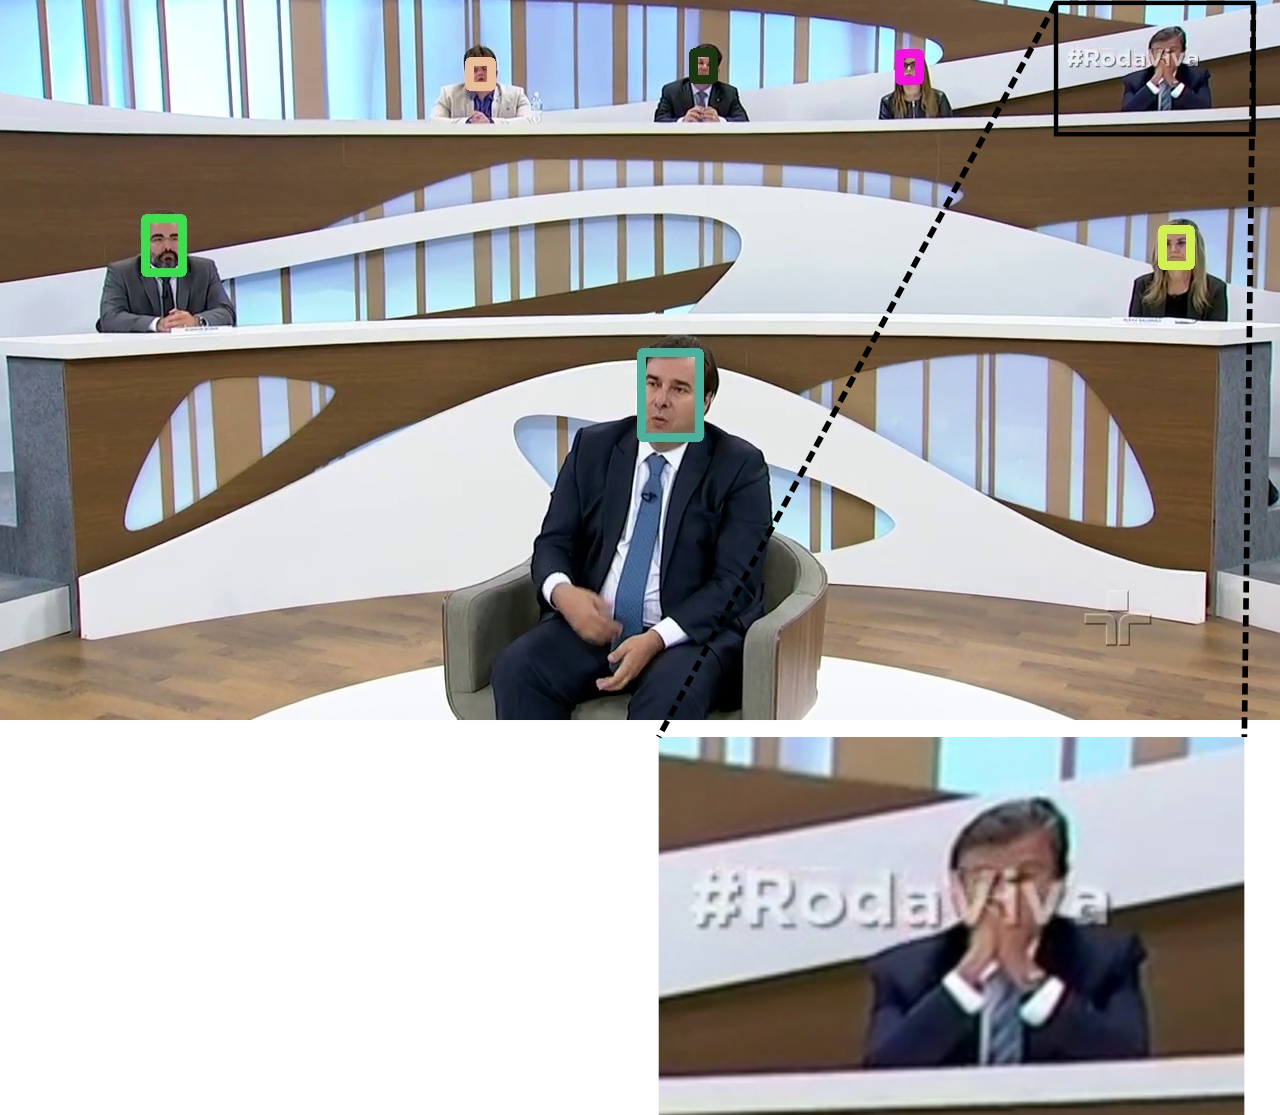
\includegraphics[width=0.9\textwidth]{img/face_recognition/maia2.png}
        \caption{Example where a face is not detected because it is covered}
        \label{fig:recall}
    \end{subfigure}\hfill
    \begin{subfigure}{0.47\linewidth}
        \centering
        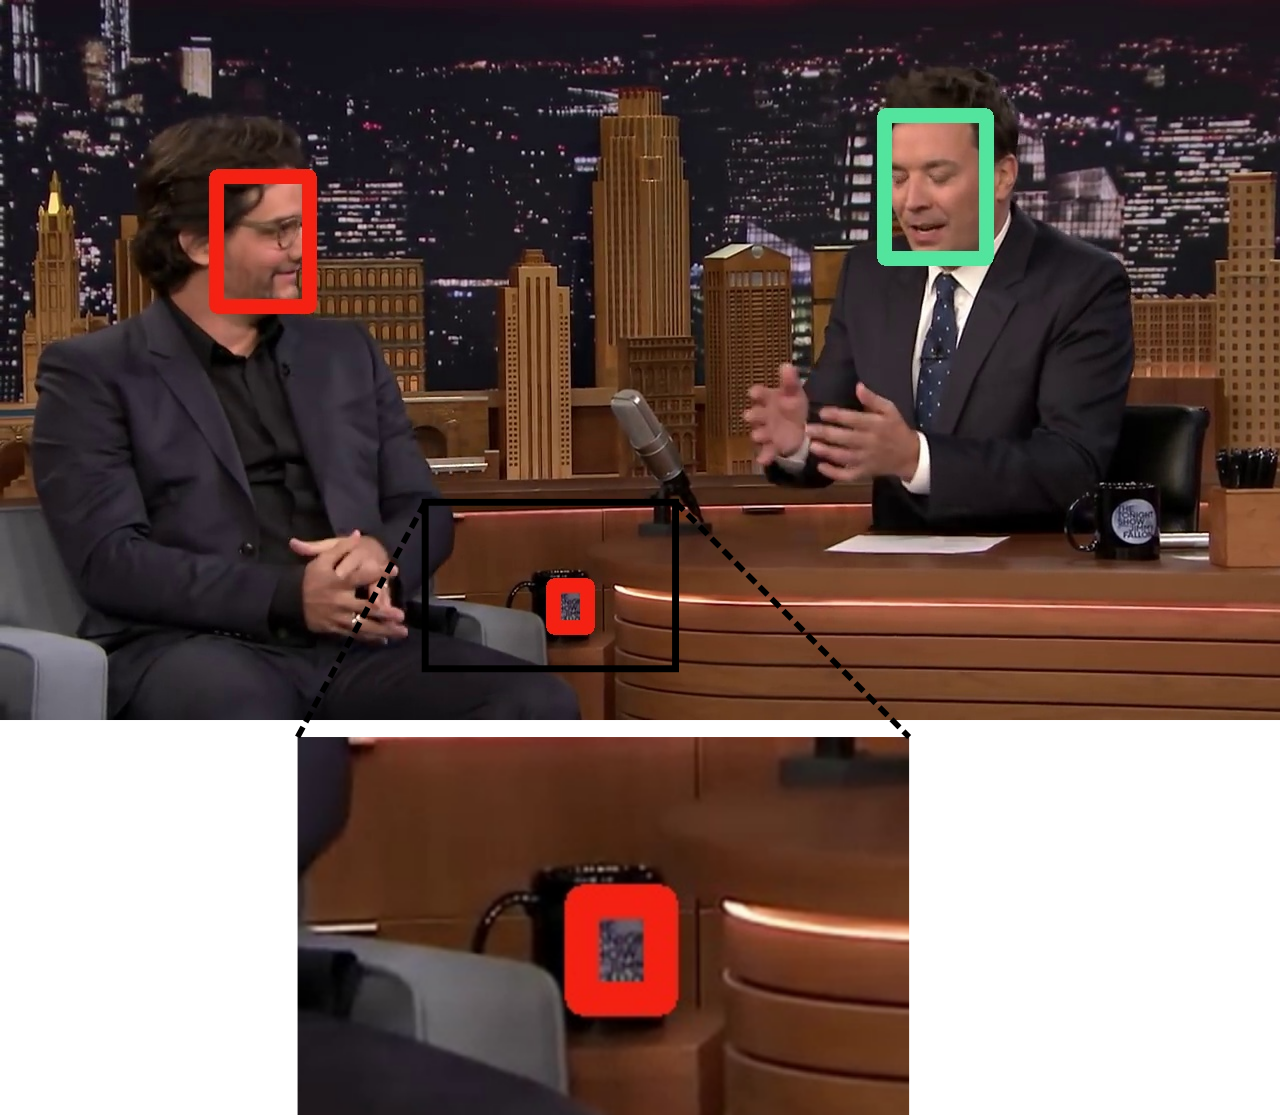
\includegraphics[width=0.9\textwidth]{img/face_recognition/wagner2.png}
        \caption{Example where a mug is detected as if it was a face.}
        \label{fig:precision}
    \end{subfigure}
\caption{Cases where our approach was incorrect.}
\end{figure}

Similar to the work of Pena \emph{et. al}~\cite{globofacestream}, our method can be used to generate metadata in video files indicating the people that appear in it.
%%
Figure \ref{fig:timeline_pol} shows the first 12 seconds of \emph{Video d}~(detailed in Table \ref{tab:results_videos}) where two identified Brazilian politicians are shown in each frame with its respective colored cluster.
\begin{figure}[!ht]
    \centering
    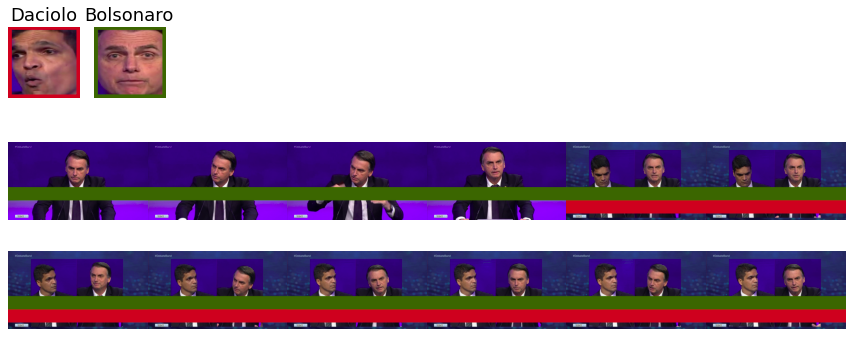
\includegraphics[width=0.8\linewidth]{img/face_recognition/timeline_pol.png}
    \caption{Timeline with tagged frames by their clusters of registered people}
    \label{fig:timeline_pol}
\end{figure}

Besides being able to recognize people in video files, by using face embeddings and clustering, we can detect the frames where the same person appears without even knowing who the person is or if he/she is in the labeled clusters.
%%
Figure \ref{fig:timeline_non_reg} shows the first 24 seconds of \emph{Video j}~(detailed in Table \ref{tab:results_videos}) with the frames tagged with the clusters identified in each frame, where each color represents a cluster.

\begin{figure}[!ht]
    \centering
    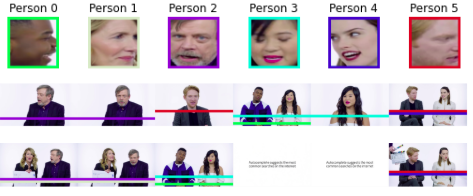
\includegraphics[width=0.8\linewidth]{img/face_recognition/timeline2.png}
    \caption{Timeline with tagged frames by their clusters of non-registered people}
    \label{fig:timeline_non_reg}
\end{figure}


\section{Discussion}
\label{sec:recognition_discussion}

\newpage
\chapter{A Clustering-Based Method for Automatic Educational Video Recommendation Using Deep Face-Features of Actors}
\label{chap:educational_recommendation}

It is a common practice among educational content creators to make collaborative videos, that is, videos in which more than one lecturer is presenting the lecture content.
%%
Such collaborations create a network of lecturers teaching a given subject.
%%
Therefore, a method that identifies these collaborations may help students find their content of interest more easily.
%%
In this chapter, we describe the second application we investigated using the \emph{Video Face Clustering} method.
%%
We propose a recommender method based on actor's presence for educational videos. In this case, the actors are lecturers~(or teachers, professors, etc.) that are presenting an educational content on video.
%%
For instance, if a student watches a video containing lecturers A and B, our method aims at recommending other videos that contain at least one of these lecturers. 
%%
This method provides an additional aid for educational recommender systems, allowing them to use the presence of lecturers as a feature for composing their recommendations.

The remainder of this chapter is structured as follows.
Section~\ref{sec:recommendation_dataset} presents the dataset we used.
We present our method in Section~\ref{sec:recommendation_method}, followed by 
%Section~\ref{sec:recommendation_experiments}, that shows the experiments to validate the face clustering and the video recommendation ranking mechanisms.
Finally, in Section~\ref{sec:recommendation_discussion}, we conclude this chapter by discussing our results.

\section{Dataset}
\label{sec:recommendation_dataset}

The experiments were conducted using a dataset created in the context of this work.
It is composed of 98 educational videos publicly available on YouTube.\footnote{\url{https://www.youtube.com/channel/UCT0JugAtGmqiYkwxFZOwAtg}}$^{,}$\footnote{\url{https://www.youtube.com/user/deboraaladim}}
%%
Each video contains at least one lecturer; moreover, some videos could have some special participation or collaboration. Therefore, the number of lecturers in each video varies from 1 to 5. In total, 16 different lecturers are present in the dataset. Each lecturer is present, in average, in 6.67\% of the videos.
%%
We also annotated the name of each lecturer present in the videos, so that we can verify if correct videos are being recommended.

%%
The videos duration vary from 00m:30s to 1h:49m:01s. 
%%
The average duration of the videos is 23m:34s, with a standard deviation of 23m:05s. 
%%
The high value of the standard deviation for the time estimates indicates that the videos are not in the same time range, and therefore have a wide duration variety. 

\section{Proposed Method}
\label{sec:recommendation_method}

Our method intends to recommend educational videos based on the lecturers that appear in each video, so that, when a person watches a video, other videos containing the same lecturers are recommended.

For doing that, we first represent each video in the dataset of educational videos by the clusters of lecturers present using \emph{Video Face Clustering}. Once we have all videos represented, we perform the pipeline depicted in Figure \ref{fig:video_recommendation}. Each of the steps of this pipeline are described in the remainder of this section.

\begin{figure}[!ht]
  \centering
  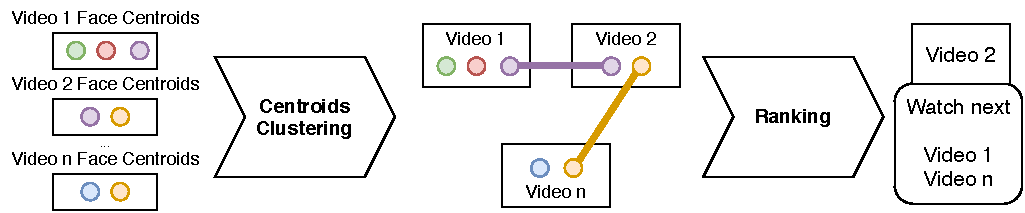
\includegraphics[width=1\textwidth]{img/video_recommendation/video_recommendation.pdf}
  \caption{Video Recommendation based on Lecturers Centroids Clustering}
  \label{fig:video_recommendation}
\end{figure}

First, we gather the centroids from the videos of the dataset as one single set and perform the \textit{Centroids Clustering}.
%%
For performing this clustering, we also use the strategy for an unknown number of clusters described in Algorithm \ref{clustering_alg}. 
%%
By doing that, we group centroids from the same lecturer that are in different videos. For instance, in Figure \ref{fig:video_recommendation}, one can see that the \emph{purple lecturer} is present in both Videos 1 and 2, while the \emph{orange lecturer} is present in both Videos 2 and n. By the end of this step, we have the group $L$ of lecturers present in the dataset of videos $V$. We also denote $L_v$ as the group of lecturers present in video $v$.

Next, based on these relationships among different videos, we perform \textit{Ranking}, by recommending videos in which lecturers of the current video are present. 
%%
For doing that, we compute a similarity score using the presence of the lecturers in the current video and the presence of these same lecturers in the other video.
%%
Let $p_{l,v}$ denote the percentage of frames in which the lecturer $l \in L_v$ is present in video $v \in V$. For each video $v \in V$ and $u \in V-v$ we compute a score of similarity $S_{v,u}$.

\begin{equation}
  S_{v,u} = \sum_{l~\in~L_v}{p_{l,v}\cdot{p_{l,u}}}
\end{equation}

Finally, using this score, for each video $v$ we compute a ranking $R_{v}$ where $R_{v,i}$ denotes the \emph{i-greatest} $S_v$ and $R_{v,i}\ge~R_{v,i+1}$ for all $i~\in~1...n_v$, where $n_v$ is the number of videos $u$ in which $S_{v,u}>~0$. 
%%
In this way, the more lecturers a video have in common with the reference video, and the more time these lecturers are present in both videos, the higher the video is positioned in the ranking of the reference video.  

By the end of this phase, we have a ranking of recommended videos for each video in the dataset.
%%
It is important to notice that our method is unsupervised and does not require the information of the lecturers in advance.
%%
Consequently, we do not store any information regarding the identity of the lecturers, respecting their privacy.


\section{Ranking Evaluation}
\label{sec:recommendation_ranking_evaluarion}

This section describes an experiment we conducted for evaluating how well our recommendation approach performed in terms of recommending relevant videos. We define that a recommendation is relevant if the reference and the recommended video have at least one lecturer in common.

First we compute the clusters that represent each lecturer in each video using \emph{Video Face Clustering}. 
%%
We start by performing \emph{Frames Extraction} for each video file using a frame rate of 1 frame per second~(fps). 
%%
Next, in the \emph{Face Detection} step, we use MTCNN \cite{mtcnn} (Multitask
Cascaded Convolutional Networks).
%%
Once we have detected the faces of lecturers in the video frames, we perform \emph{Embeddings Generation} using SeNet-50 \cite{senet} that generates embeddings on the $\mathbb{R}^{2048}$ feature space. 
%%
We used the architecture and weights pre-trained on the VGGFace2 dataset~\cite{cao2018vggface2}.
%%
Finally, in the \emph{Clustering} step, since we do not know the number of clusters in advance, we used the strategy described in Section \ref{subsec:unknown_nclusters} with $t=5$, $\omega=0.2$, that empirically demonstrated good results. For the \texttt{Clustering} procedure, we used Agglomerative Clustering~\cite{ward1963hierarchical}.
%%
The choice of using SeNet-50 and Agglomerative Clustering comes from the fact that this combination achieved the best results in the experiment described in Section \ref{sec:recognition_clustering_validation}.

For performing the video recommendation task, we gather the centroids~(that represent each lecturer in the video) from all videos in the dataset. Next, we perform the process described in Section \ref{sec:recommendation_method}. For \emph{Centroids Clustering}, we also use Algorithm \ref{clustering_alg} with the same parameters $t=5$, $\omega=0.2$, and the Ward Aglommerative Clustering as \texttt{Clustering} procedure. Finally, based on the clusters generated, we perform the \emph{Ranking} step

To evaluate our ranking, for each video we compute the Average Precision~(AP), that evaluates how well a ranking of recommendations is based on each element's relevancy. 
%%
This metric penalizes more a ranking if a non-relevant element is recommended in the first positions than if it was in the last ones.
%%
Let $P_k$ be the precision of the first $k$ elements of a ranking, which is the percentage of videos that are relevant in the sub-ranking that starts at position $1$ and ends at position $k$.
%%
Let $\alpha_k$ denote the relevancy of the video in position $k$, where $\alpha_k = 1$ if the video is relevant, and $0$ otherwise.
%%
The AP of a given ranking is defined as follows
\begin{equation}
  \label{equation:average_precision}
  AP = \frac{1}{GTP}\sum_{k=1}^{n}{P_k~\cdot~\alpha_k}
\end{equation}
where GTP refers to the total number of ground truth positives in the ranking, which is the total number of videos that are considered relevant in a ranking. Figure \ref{fig:ap_example} shows an example of how the AP is computed for a given ranking. In this case, the $GTP=3$ because the total number of relevant videos in the ranking is 3~(videos A, B and D).

\begin{figure}[ht]
  \centering
  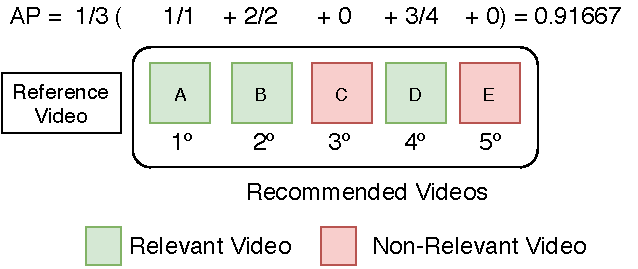
\includegraphics[width=0.7\linewidth]{img/video_recommendation/ap_example.pdf}
  \caption{Example of how the Average Precision~(AP) is computed for a reference video and its recommended videos.}
  \label{fig:ap_example}
\end{figure}

In order to prevent outliers from having much influence in the recommendation (e.g. a person that is not a lecturer -- and not relevant to the video -- and appears for a short amount of time), we experimented different thresholds of presence intervals in a video for a person to be considered as ``present'' when computing the score for the ranking. 
%%
In this way, a $p_{l,v}$ lesser than the threshold is considered as $0$.
%%
Besides the Average Precision, we also compute the mean and minimum values of the recall~(MeanR), precision~(MeanP), and F1-Score~(MeanF1) for the recommendation generated for each of the videos, without considering the positioning of these videos in the rankings.
%%
The recall refers to the percentage of relevant videos that are present in the ranking.
%%
The F1-score represents an overall performance metric based on the  harmonic mean of the precision and recall and is defined as follows.
\begin{equation}
    \label{equation:f1}
    F1 = \frac{2 \cdot P \cdot R}{P + R}
\end{equation}
Table \ref{tab:results} shows the thresholds used, the values of recall, precision, F1-score, and the Mean Average Precision (mAP).

One can observe from Table \ref{tab:results} that the precision clearly increased with the use of the threshold.
%%
Different from the precision, the recall decreased with the increase of the threshold. It means that with a greater threshold more videos that should be recommended were not chosen by our method.
%%
It is important to notice that these two metrics~(precision and recall) do not consider the ordering of the recommendations.
%%
Different from them, the Mean Average Precision~(mAP) has high values for all thresholds, specially because the score for computing the ranking takes into consideration the percentage of time that a person appears in the reference and recommended videos.
%%
Then, we can conclude that our proposed approach for ordering the recommended videos tends to recommend more suitable videos first with a high mAP$\approx0.99$. 

\begin{table*}[!ht]
\small
\centering
\caption{Results obtained with our approach with different thresholds of time presence for a lecturer to be considered as present in a video.}
\label{tab:results}
\begin{tabular}{ccccc}
\hline
\textbf{Thershold} & \textbf{MeanR}  & \textbf{MeanP} & \textbf{MeanF1} &\textbf{mAP} \\ \hline
0\%                & 0,88851         & 0,64681        & 0,70971         & 0,98641   \\
1\%                & 0,88851         & 0,64681        & 0,70971         & 0,98641   \\
2\%                & 0,88851         & 0,64885        & 0,71171         & 0,98641   \\
3\%                & 0,88851         & 0,67368        & 0,73086         & 0,98642   \\
4\%                & 0,88851         & 0,67368        & 0,73086         & 0,98642   \\
5\%                & 0,88851         & 0,69923        & 0,74930         & 0,98642   \\
6\%                & 0,88851         & 0,73615        & 0,77648         & 0,98642   \\
7\%                & 0,88742         & 0,77849        & 0,80768         & 0,98642   \\
8\%                & 0,88742         & 0,78408        & 0,81111         & 0,98643   \\
9\%                & 0,88742         & 0,80171        & 0,82410         & 0,98643   \\
10\%               & 0,88742         & 0,83165        & 0,84306         & 0,98643   \\
11\%               & 0,88742         & 0,85306        & 0,85693         & 0,98643   \\
12\%               & 0,88616         & 0,85956        & 0,86018         & 0,98662   \\
13\%               & 0,88490         & 0,88216        & 0,87305         & 0,98688   \\
14\%               & 0,88289         & 0,90265        & 0,88450         & 0,98884   \\
15\%               & 0,88289         & 0,90265        & 0,88450         & 0,98884   \\
16\%               & 0,88163         & 0,91327        & 0,88980         & 0,98908   \\
17\%               & 0,87197         & 0,91538        & 0,88580         & 0,98912   \\
18\%               & 0,87197         & 0,91538        & 0,88580         & 0,98912   \\
19\%               & 0,87086         & 0,93165        & 0,89476         & 0,98946   \\
20\%               & 0,86130         & 0,93645        & 0,89218         & 0,99000   \\
21\%               & 0,86130         & 0,93645        & 0,89218         & 0,99000   \\
22\%               & 0,86130         & 0,95054        & 0,89886         & 0,99000   \\
23\%               & 0,86130         & 0,95054        & 0,89886         & 0,99000   \\
24\%               & 0,85805         & 0,95718        & 0,90046         & 0,99165   \\
25\%               & 0,85805         & 0,95718        & 0,90046         & 0,99165  
\end{tabular}
\end{table*}

\section{Discussion}
\label{sec:recommendation_discussion}

In this chapter, we present a method for educational video recommendation using \emph{Video Face Clustering}. More precisely, we use an unsupervised clustering-based method and an heuristic for ranking.
%%
It takes advantage of face detection mechanisms to perform educational video recommendation based on the lecturers' presence.
%%
Besides the face detection, we also perform face clustering of the lecturers in each video, and, given these clusters, we extract their centroids to perform another clustering step that creates a relationship of videos that share the presence of the same lecturers.
%%
Finally, we rank the recommended videos based on the amount of time each lecturer is present.
%% 
It is worth mentioning that our method is completely automatic and does not require any information of the video files in advance.  
%%
Moreover, our approach does not need to know or store the identity of the lecturers for performing recommendation, preserving their privacy.

A collateral contribution of this application is video segmentation by lecturers.
As illustrated in Figure \ref{fig:video_timeline}, we can create a timeline based on lecturers' presence, which can be used to help students in finding moments where specific lecturers are present.
%%
With this segmentation, we could recommend specific parts of the video to the student.

\begin{figure}[!ht]
  \centering
  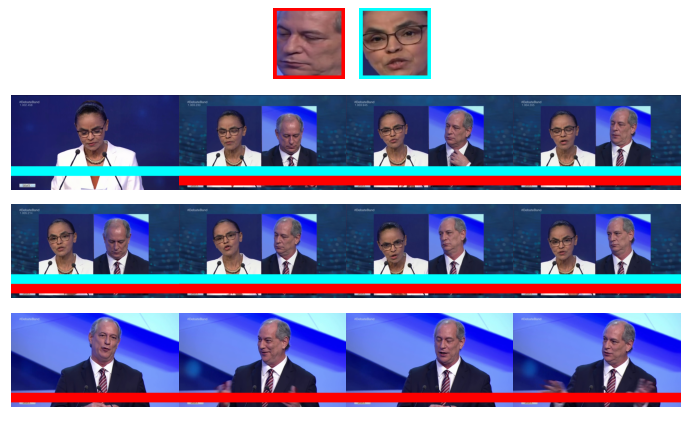
\includegraphics[width=0.8\linewidth]{img/face_clustering/example_localization.png}
  \caption{Educational video timeline tagged by the lecturers presence. Notice that the frames with the lecturer on the left are tagged in red, while the frames with the lecturer on the right are tagged in yellow.}
  \label{fig:video_timeline}
\end{figure}

The main limitation of our method is that we can only recommend videos in which the lecturers are visually present. However, this method can be used in a hybrid recommendation approach, that combines both textual and audiovisual information from the video to create clusters. 
\newpage
\chapter{Video Face Clustering for Subtitles Positioning in 360-Videos}
\label{chap:subtitles_positioning}

In \cite{mendes2020authoring}, we proposed an authoring model for interactive 360-video. In such a model, we can define interactive 360-videos that are presented together with additional information attached to it, such as image, text, 2D traditional videos and spatial audio. The positioning of such information is defined by their polar coordinates, start time and duration. For instance, we can define that a text moves with the user's head motion and is always visible or that such text is placed at a fixed position if its in user's the field of view. In this chapter we describe how \emph{video face clustering} can be used together with this authoring model for automatic subtitles positioning in 360-video. Section \ref{sec:authoring_clustering_360} describes how we adapt \emph{video face clustering} for the context of 360-videos. In Section \ref{sec:authoring_model}, we describe the authoring model we proposed that together with face clustering can be used for automatic positioning subtitles in 360-videos.
 
\section{Video Face Clustering in 360-Videos}

\label{sec:authoring_clustering_360}

Nowadays, the most common way for representing and transmitting 360-video is using an equirectangular projection~\cite{yang2018object}. With the equirectangular projection, each sphere point is defined by two angles~\cite{snyder1987map}: \emph{latitude}~$\theta \in [-90^{\circ}, +90^{\circ}]$ and \emph{longitude}~$\phi \in [-180^{\circ}, +180^{\circ}]$. This kind of projection creates challenges for image processing and computer vision algorithms, especially to the convolution-based ones because of the severe distortions in areas vertically distant from the center of the image~(see Figure \ref{fig:equirectangular_proj}). Due to these distortions, we adapted the \emph{Face Detection} step of our method which uses a traditional CNN. Section \ref{subsec:360_face_detection} describes how we adapted the \emph{Face Detection} step to the 360-video context.

\begin{figure}[!ht]
\centering
    \begin{subfigure}{0.47\linewidth}
        \centering
        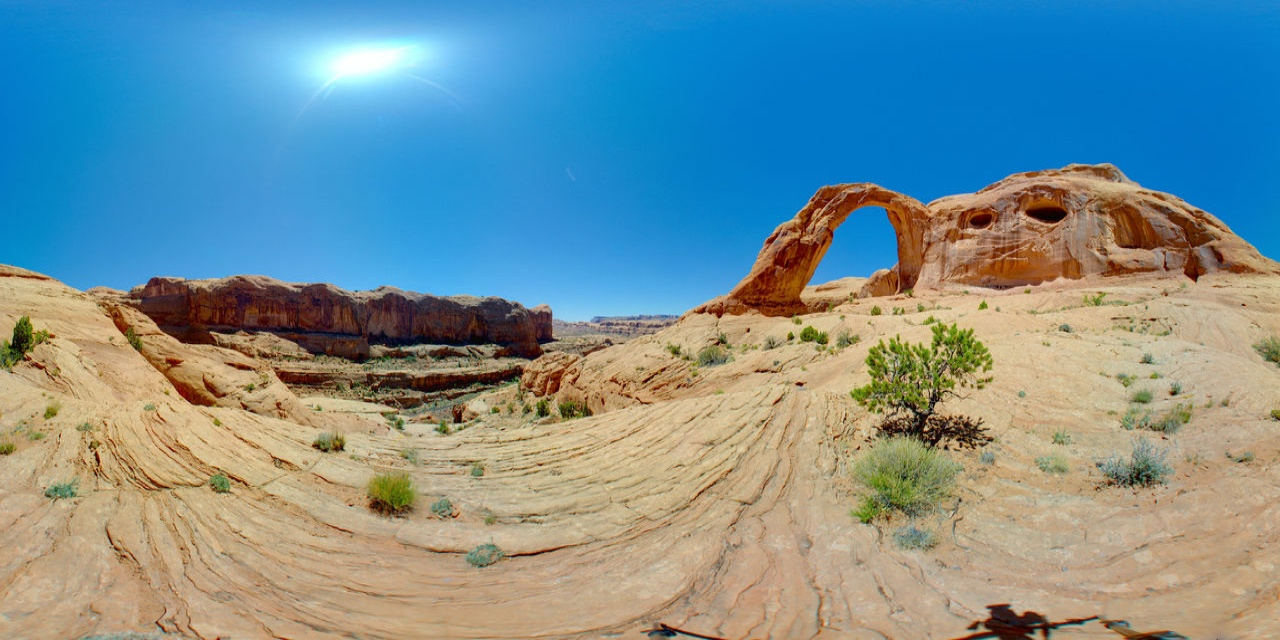
\includegraphics[width=1\textwidth]{img/video360/equi_outdoor.jpg}
        \caption{Outdoor equirectangular image.}
        \label{subfig:out_equi}
    \end{subfigure}\hfill
    \begin{subfigure}{0.47\linewidth}
        \centering
        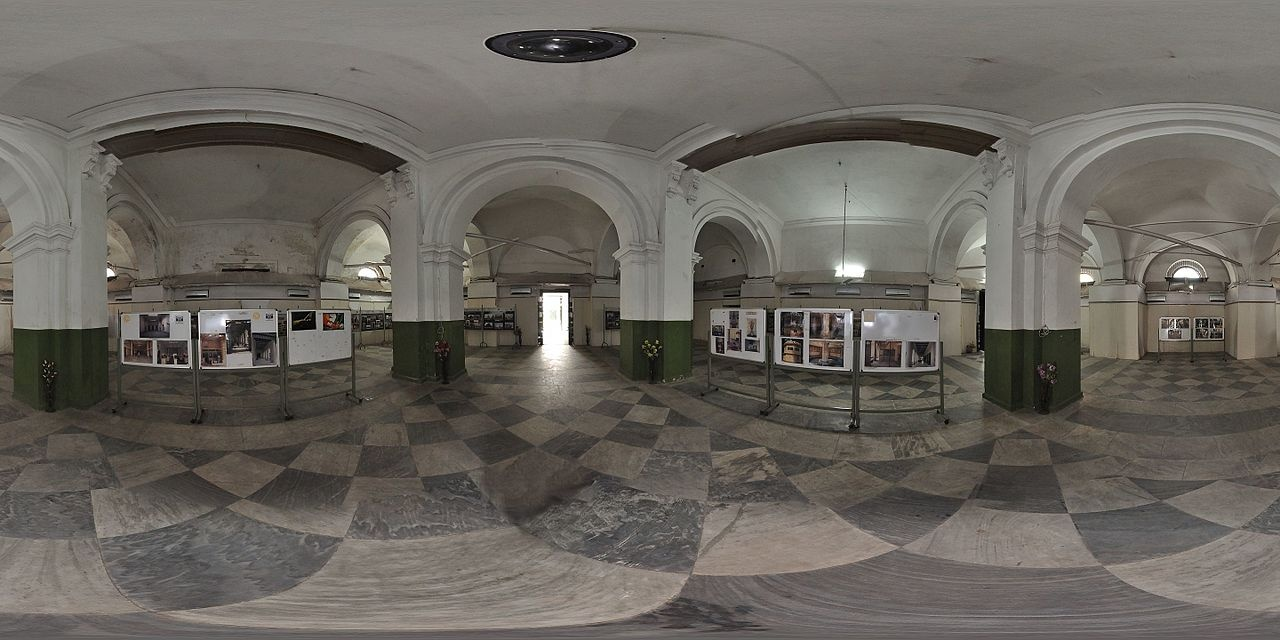
\includegraphics[width=1\textwidth]{img/video360/equi_indoor.jpg}
        \caption{Indoor equirectangular image.}
        \label{subfig:in_equi}
    \end{subfigure}

\caption{Examples of 360-images represented through equirectangular projection.}
\label{fig:equirectangular_proj}
\end{figure}

\subsection{Face Detection in Equirectangular 360°}
\label{subsec:360_face_detection}

In order to mitigate the problem of severe distortions present in the equirectangular projection, we have used an approach based on viewports extraction. Figure \ref{fig:360_face_detection} shows this process and each of its steps is explained in the following paragraphs.

\begin{figure}[!ht]
    \centering
    
\includegraphics[width=1\linewidth]{img/video360/360facedetection.pdf}
    \caption{360-degree face detection process.}
    \label{fig:360_face_detection}
\end{figure}

Given an equirectangular image, which could also be a frame from a 360-video, we first perform \emph{Viewports Extraction}. A viewport represents a portion of the 360-degree scene~(see Figure \ref{fig:authoring_exviewport}), it is similar to when a person takes a picture in the real world. The picture represents the world from a point of view towards a specific direction. A viewport is defined by its center, in polar coordinates (lat, long), its field of view~(FoV), and the width or height of the resulting image. The FoV, given in degrees, is the extend of the 360-image that is present in the viewport.

\begin{figure}[!ht]
    \centering
    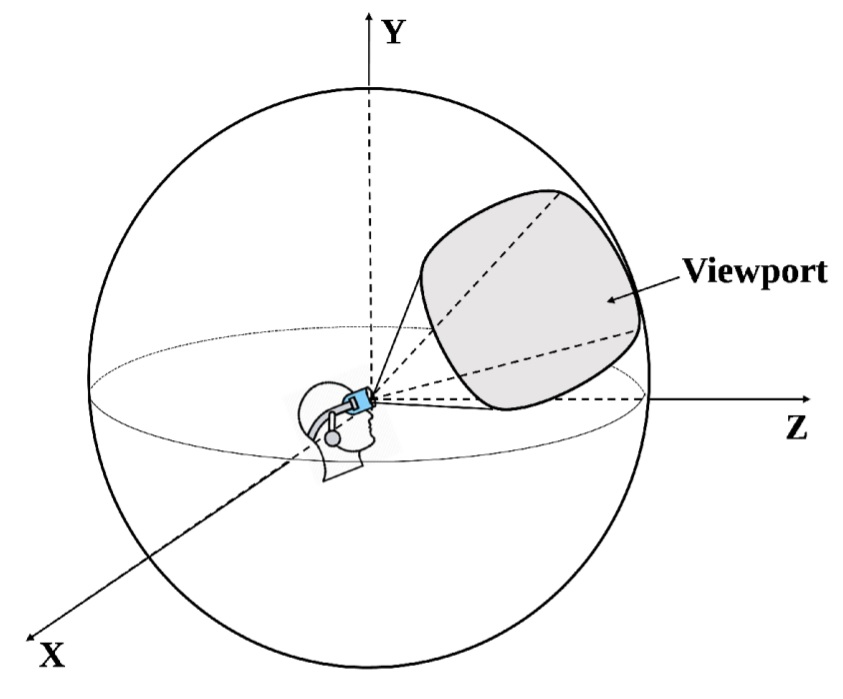
\includegraphics[width=0.5\linewidth]{img/video360/viewport.jpg}
    \caption{Example of a viewport from a 360-video. Extracted from \cite{nguyen2020evaluation}.}
    \label{fig:authoring_exviewport}
\end{figure}

Because we want the viewports to cover the greatest possible area from the 360-degree image, our method receives two parameters: the viewports' \emph{density}~(\emph{d}) and \emph{FoV}. The \emph{density} is equal to the number of viewports in the latitude range. Proportionally, the number of viewports in the longitude range is equal to double the \emph{density}. Figure \ref{fig:authoring_viewports} shows viewports extracted from Figure \ref{subfig:out_equi} with \emph{density}=3 and FoV=60°. As the density was equal to three, the number of viewports is three in the latitude's range and six in the longitude's range. In total, 18 viewports were extracted in the example bellow.

\begin{figure}[!ht]
    \centering
    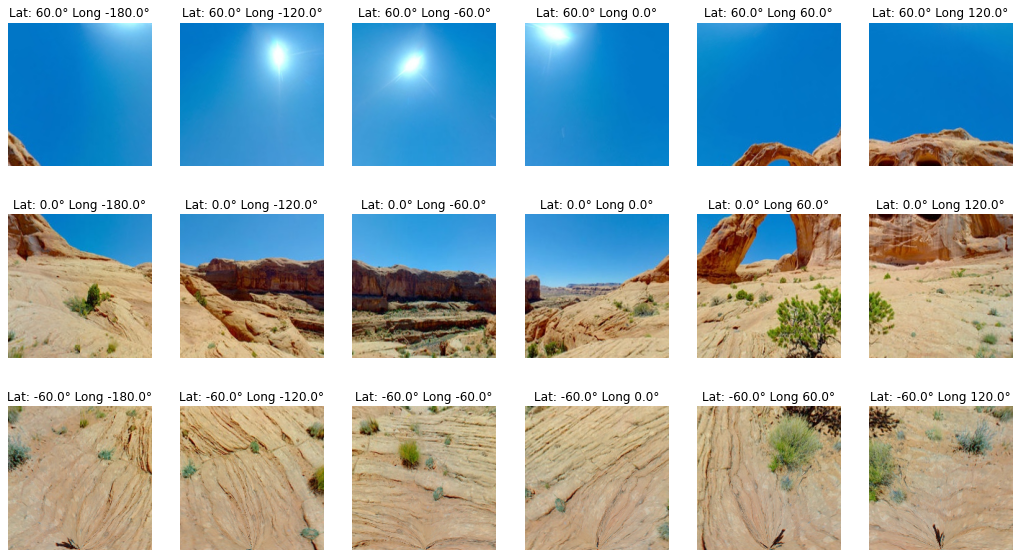
\includegraphics[width=1\linewidth]{img/video360/viewports.png}
    \caption{Viewports extracted from Figure \ref{subfig:out_equi} with \emph{density}=3 and FoV=60°.}
    \label{fig:authoring_viewports}
\end{figure}

With these viewports, we hope to reduce the distortions since we are representing the equirectangular image with a series of standard images, similar to the ones used by traditional CNNs. Next, for each of these viewports we perform \emph{Face Detection} using a traditional CNN. Then, for each viewport we have a group of faces detected.

In the last step of our approach, called \emph{Mapping}, we map each face detected back to the equirectangular image. One can notice that some parts of the equirectangular image are present in more than one viewport. Notice that the sun is present in three viewports in the first line of Figure \ref{fig:authoring_viewports}. In order to avoid repeated detections in the equirectangular image, we use the Non-Maximum Supression~(NMS) Algorithm. This algorithm eliminates overlapping bounding boxes within a given threshold and is widely used in object detection algorithms~\cite{nms1, nms2, nms3, nms4, nms5}.

We evaluated this approach in comparison to applying a detection model directly to the equirectangular image. We searched for datasets for face detection in equirectangular 360-images. However, by the time of our search, he have not found any. For that reason, we decided to create a synthetic dataset to perform this evaluation. 
%%
Similar to \cite{fu2019fddb}, we created a synthetic dataset based on the FDDB dataset~\cite{jain2010fddb}. In \cite{fu2019fddb}, the authors create a synthetic dataset for face detction in 360-degree fisheye images. Ours, differently, aims at equirectangular images, projecting rectilinear images to the equirectangular projection.

The FDDB dataset~\cite{jain2010fddb} is a popular benchmark for face detection evaluation containing 2845 images and 5171 faces. We collected 19 indoor and outdoor equirectangular images from Google Images,\footnote{\url{https://www.google.com/imghp}} ESO,\footnote{\url{https://www.eso.org/public}} and PxHere\footnote{\url{https://pxhere.com}} to use as background.
%%
For each image in the FDDB dataset, we randomly chose a latitude, longitude and equirectangular background image to project it.
%%
For each face present on the FDDB image, we projected its bounding box to the new equirectangular synthetic image. Figure \ref{fig:authoring_fddb_proj} shows an example of an image from FDDB projected in the polar coordinates \emph{lat} $ = -60^{\circ}$ \emph{long} $ = 0^{\circ}$ to an equirectangular image.

\begin{figure}[!ht]
\centering
    \begin{subfigure}{0.4\linewidth}
        \centering
        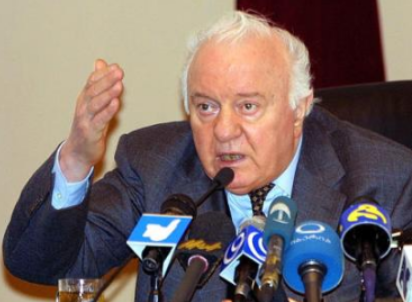
\includegraphics[height=9em]{img/video360/face_pre.png}
        \caption{FDDB image example.}
        \label{subfig:face_pre}
    \end{subfigure}\hfill
    \begin{subfigure}{0.55\linewidth}
        \centering
         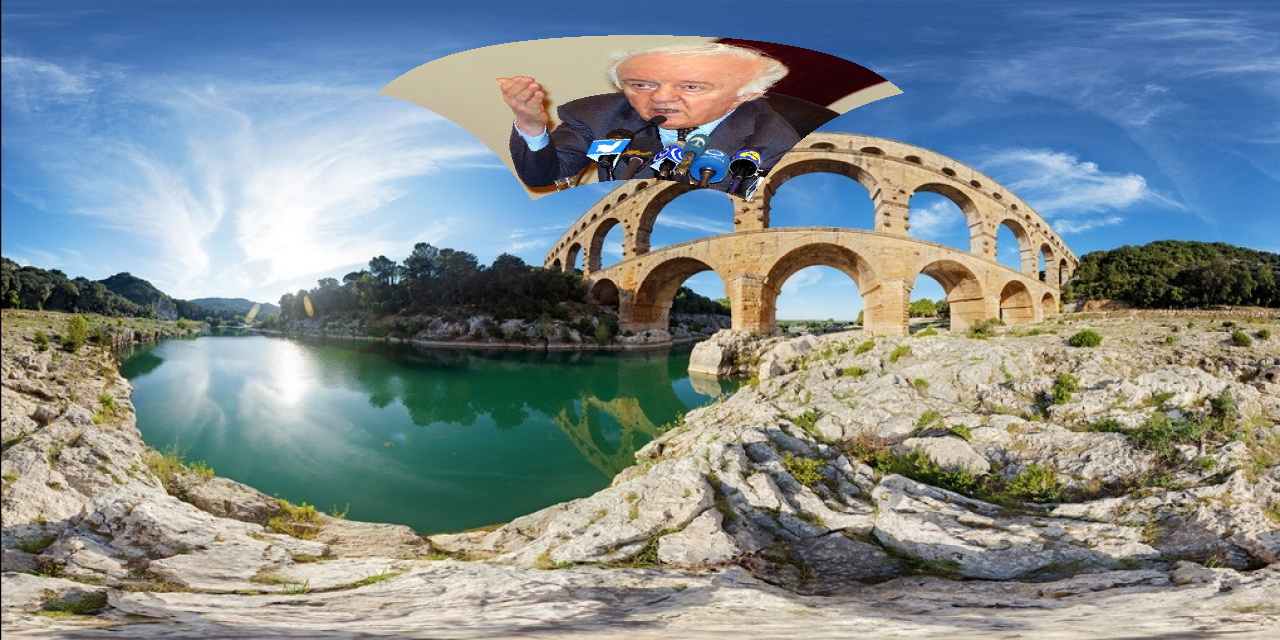
\includegraphics[height=9em]{img/video360/face_pos.png}
        \caption{Projection example of FDDB image.}
        \label{subfig:face_pos}
    \end{subfigure}

\caption{FDDB image projection to Equirectangular image.}
\label{fig:authoring_fddb_proj}
\end{figure}

Depending on the position that the rectilinear image is projected, the distortions are more or less severe. The distortions increase as the projection vertically distances from the center of the image. Figure \ref{fig:different_projections} shows different resulting equirectangular images depending on the position that the rectilinear image is projected. Notice that the projections vertically close to the border of the image have more distortions than the ones close to the center of the image.

\begin{figure}[!ht]
    \centering
    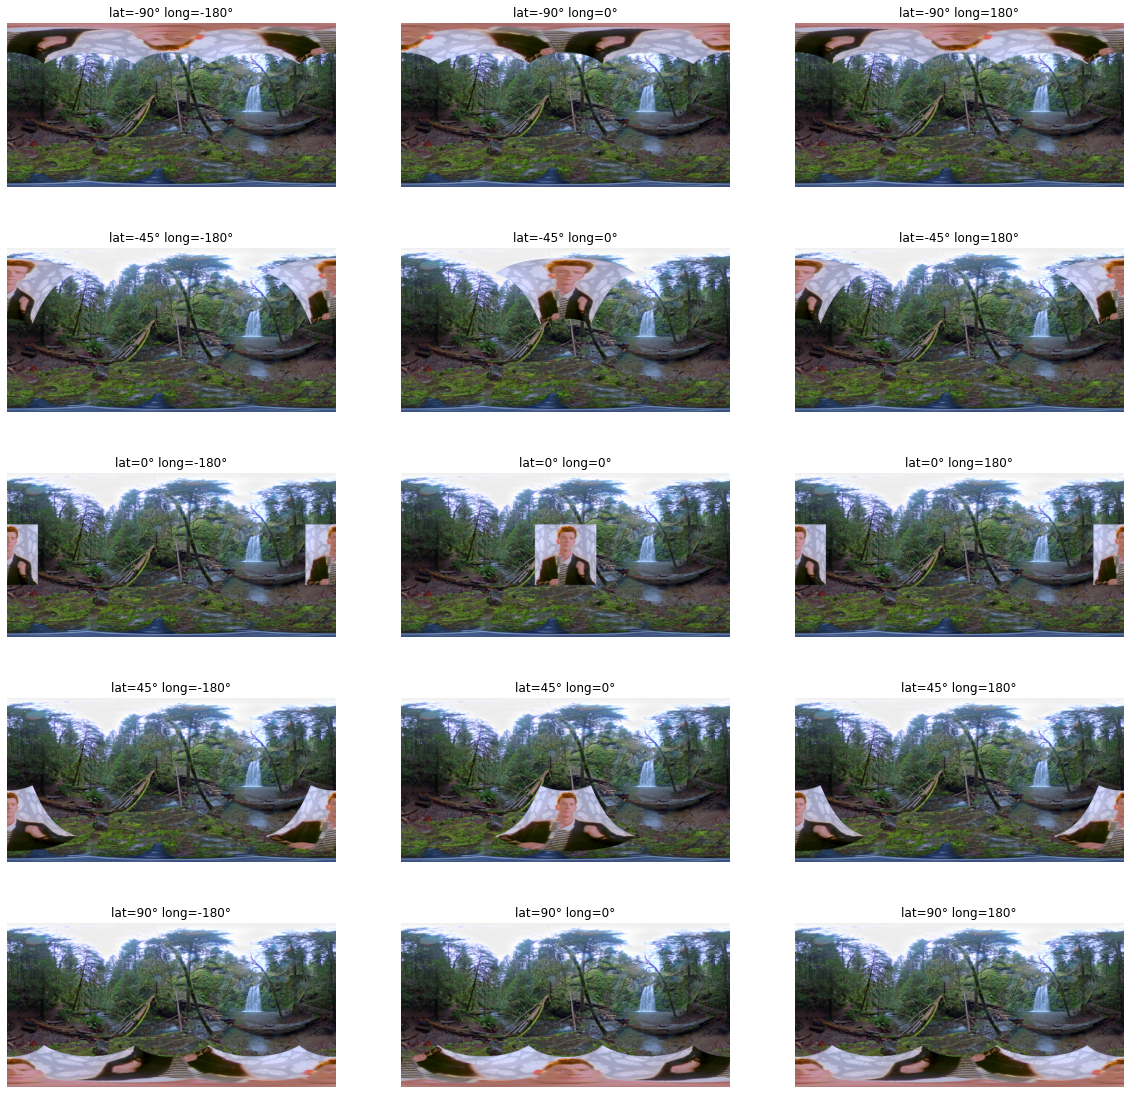
\includegraphics[width=0.9\linewidth]{img/video360/different_projections.png}
    \caption{Different resulting synthetic equirectangular images depending on the position that the rectlinear image was projected.}
    \label{fig:different_projections}
\end{figure}

We evaluated our approach in the synthetic dataset using MTCNN\cite{mtcnn} as the model for face detection. We compare the usage of MTCNN alone, directly in the equirectangular images, against MTCNN with viewports. For the MTCNN with viewport, we used extracted viewports with \emph{density}=3 and FoV=60°. We evaluated both methods using the Mean Average Precision~(mAP) that is widely used for the object detection task~\cite{map1, map2, map3, map4}. 


From Figure \ref{fig:different_projections}, one can notice that a greater module of the latitude~($|lat|$) implies in more severe distortions, as the projection is more vertically distant from the center of the equirectangular image. Figure \ref{fig:results_360_detection} shows the results we obtained for MTCNN and MTCNN with viewports. 
We vary the x-axis of the chart so that we consider only the synthetic equirectangular images whose projection's $|lat|$ is greater or equal than each x. In this way, a greater x means a more difficult subset of images from our synthetic dataset. The mAP value for MTCNN drops drastically as we start considering only more and more difficult images. In contrast, with the use of viewports, the mAP value still decreases but at slower pace. Besides achieving better results, one of the main advantages of this technique is that it can be used with a model that was trained for detecting faces in traditional rectlinear images.

\begin{figure}[!ht]
    \centering
    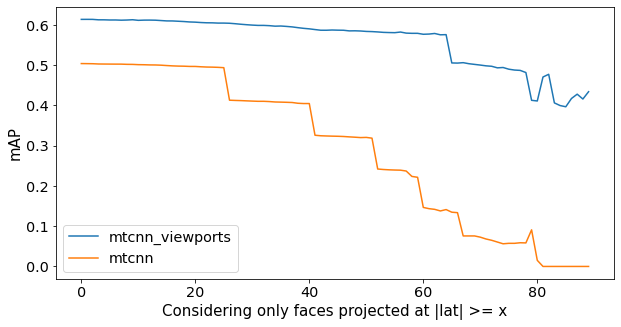
\includegraphics[width=0.8\linewidth]{img/video360/results_360_detection.png}
    \caption{Face detection results using MTCNN and MTCNN with viewports.}
    \label{fig:results_360_detection}
\end{figure}

With this adaptation, we are able to use \emph{Video Face Clustering} for 360-video. To do that, in the \emph{face detection} step we use the viewports strategy with MTCNN. 


\section{An Authoring Model for Interactive 360-Videos}
\label{sec:authoring_model}

In this section, we describe an authoring model for interactive 360-videos. Although the model is not entirely used for subtitles positioning in 360-videos, we describe it completely because the development of such authoring model was part of the researches conducted during our master research.

Despite the limited ``look around'' interactivity supported by traditional 360
videos and HMDs, \emph{interactive 360
videos}~\cite{chambel2011,berning2013parnorama} support additional interactive
elements, such as overlaid 2D/3D information, hyperlinks, and additional input
elements.
%%
Such features allow an enhanced user experience, supporting applications such
as remote operations and telepresence, museums, immersive interactive
narratives, and improve educational content.
%%
Most of the current 360 video streaming services, however, still do not
support such interactive features for 360 videos.
%%
Indeed, when compared to its 2D-only video counterpart, although most of the
popular streaming services~(e.g., Youtube and Facebook) offer tools to create
interactive 2D videos (\emph{e.g.}, to insert additional information,
subtitles, and hyperlinks), they lack similar tools to create interactive 360
videos.

We propose a declarative authoring model that allows authors to design and create interactive 360 videos.
%%
First, we analyze different scenarios of immersive multimedia applications
based on 360 videos with the aim of extracting the main requirements for such
an authoring model.
%%
Then, based on the gathered requirements, we propose an XML-based declarative
model that allows authors to design and create 360 interactive videos.

\subsection{Scenarios and requirements}
\label{subsec:authoring_scenarios}

The following target scenarios are used to gather the requirements for our
authoring model for interactive 360 videos.

\textbf{360 hypervideo}.
%%
This scenario is characterized by navigation among 360 videos, and can be useful, for instance, in entertainment or educational context~(see Figure \ref{fig:cenario_hiper}).
%%
The user can navigate from the current to another 360 video, while the current
one proceeds in a ``preview mode''.
%%
Besides the support for navigation between 360 degree videos, it should be
possible to add overlaid information to it~(e.g., image, video, text) to
enhance its viewing experience.
%%
An example of such a scenario is a virtual tour in a museum, where the user
may navigate through different rooms.
%%
Each room could have additional information about the presented piece of art.
%%
Another example is virtual learning environment, in which the user can navigate among different topics and learn more about each of them with additional information.

\begin{figure}[!ht]
    \centering
    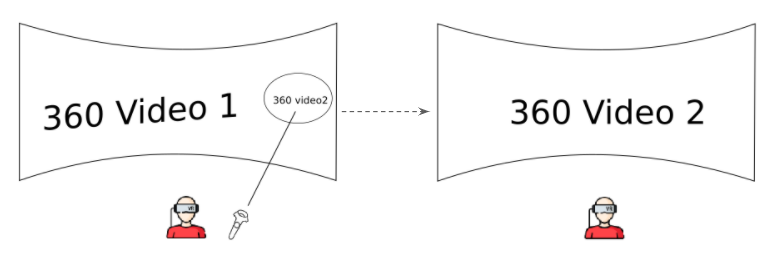
\includegraphics[width=0.8\linewidth]{img/video360/hyper.png}
    \caption{360 hypervideo scenario.}
    \label{fig:cenario_hiper}
\end{figure}

\textbf{Accessible 360-video}. 
%% 
In this scenario, a 360 video is presented together with its translation in either sign language or subtitles~(see Figure \ref{fig:cenario_acessivel}).
%%
For the sign language case, both a 2D regular video using Picture-in-Picture~(PiP) or a 3D human model could be displayed.
%%
Such a scenario intends to provide an immersive experience for people with hearing disabilities.
%%
An example is a voice-based virtual tutorial for managing a machine in a factory that can support sign languages or subtitles to allow the inclusion of people with hearing disabilities.

\begin{figure}[!ht]
    \centering
    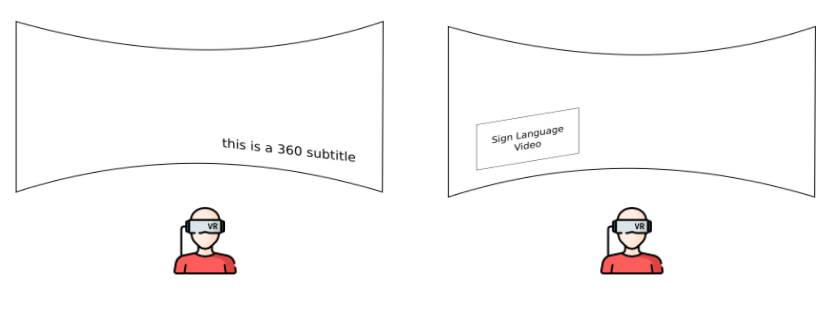
\includegraphics[width=0.8\linewidth]{img/video360/accessible.png}
    \caption{Acessible 360-video scenario.}
    \label{fig:cenario_acessivel}
\end{figure}

\textbf{360-video with guided attention}.
%%
In this scenario, a 360 video has a recommended region to look at.
%%
Whenever the user is not looking at the recommended region, additional guiders
(e.g., arrows) can be rendered informing the user to where he should be
looking in the 360 video~(see Figure \ref{fig:cenario_guiado}).
%%
Also, a live view of it can be presented in picture-in-picture~(PiP) in part
of the field of view; thus, providing the user with key content, whether he/she is looking at it or
not.
%%
Besides visual cues, spatial audio cues are also important in virtual
environments and can help in guide users' attention.
%%
Thus, the audio of the 360-degree video may come from the recommended
position, in a way that it sounds different depending on the position the user
is looking at. 
%%
To support such a scenario, it should be possible to detect if the user is
looking at a specific direction of the scene and to render another segment of
the video using PiP.
%%
The region of interest of a 360 degree video is content dependent, thus the
producer should be able to customize it towards providing the best possible
user experience.
%%
An example of such a scenario is a lecture, in which the recommended position
to look at is where the lecturer may be located, e.g. the stage.

\begin{figure}[!ht]
    \centering
    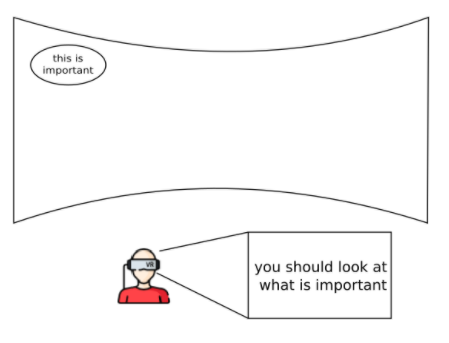
\includegraphics[width=0.4\linewidth]{img/video360/guided.png}
    \caption{360-video with guided attention scenario.}
    \label{fig:cenario_guiado}
\end{figure}

Based on the above target scenarios, we can extract requirements addressing
presentation~(RP) and interaction~(RI) that should be
supported by an authoring model for 360 interactive videos, which are detailed
in the following.

\begin{itemize}
    \item \textbf{RP.1 Overlaid information}. Additional media objects
      (video, image, sound, and text) might be positioned in the 360-degree
      environment.
   \item \textbf{RP.2 Styling}. Different media elements may share the same
      position and presentation characteristics.
      %%
      Thus, the author should be able to reuse the same style in different
      elements.
  \item \textbf{RP.3 3D Audio}. A 3D audio manipulates the sound delivered by
    stereo speakers or headphones, creating the idea that the audio is coming
    from a specific direction.
  \item \textbf{RP.4 Subtitles}. Support subtitles both world referenced and fixed to the user.
  \item \textbf{RP.5 360 Spatial Layout}. The media elements should use a
    360-based coordinate system, whereas the viewer camera is the center.
  \item \textbf{RP.6 Presentation Timing}. The media elements should be
    presented synchronized with the 360 video of the scene. 
  \item \textbf{RI.1 Navigation}. This requirement intent to enable users
    navigate between 360 videos. This also includes show to users preview of
    possibles videos to visit.
  \item \textbf{RI.2 Hotspot}. This requirement defines a position in the
    360-degree scene in which different actions can be performed when the user
    looks at it or is not looking at it.
  \item \textbf{RI.3 Viewport preview}. This requirement refers to the use of
    a picture-in-picture live view at the user's current viewport, rendering
    an important section of the 360-degree scene defined by a \emph{hotspot}.
\end{itemize}



\subsection{Proposed model}
\label{subsec:proposal}
 
To full-fill the aforementioned requirements, we propose an authoring model that allows authors to design and create 360 interactive videos. Table~\ref{tbl:entities} presents the entities of the model.
\begin{table}[!ht]
\footnotesize
\begin{tabularx}{\linewidth}{ p{3cm} p{4cm} X }
\hline

\textbf{element} & \textbf{children} & \textbf{attributes}\\ \hline

\textbf{\emph{presentation360}}  & \emph{head}, \emph{\emph{body}} &  \\ \hline

\textbf{\emph{head}}  & \emph{style} &  \\  \hline

\textbf{\emph{style}}  &  & * \\  \hline

\textbf{\emph{body}}  & \emph{scene360}+ & entry \\ \hline

\textbf{\emph{scene360}}  & \emph{text}*, \emph{image}*, \emph{video}*,
\emph{subtitle}*, \emph{preview}*, \emph{hotspot}*, \emph{mirror}* & src, volume? \\  \hline

\textbf{\emph{text}, \emph{image}}  &  & 
id, src, r?, phi?, theta?, tpos?, style?, begin?, dur?, followCamera?, onselect? \\ \hline

\textbf{\emph{audio}, \emph{video}, \emph{subtitle}, \emph{preview}}  &  & 
id, src, r?, phi?, theta?, tpos?, style?, begin?, dur?, followCamera?, onselect?, clipBegin?, clipEnd?\\ \hline

\textbf{\emph{mirror}}  &  & 
id, src, r?, phi?, theta?, tpos?, style?, begin?, dur?, 
followCamera? \\ \hline

\textbf{\emph{hotspot}}  &  & 
id, src, r?, phi?, theta?, tpos?, 
style?, begin?, dur?,  onLookAt?, duringNotLookingAt?, onSelect? \\ \hline

\hline
 \end{tabularx}
\caption{Elements BNF. Conventionally: a \emph{plus sign} (+) indicates that the element can occur one or more times. The \emph{asterisk} (*) indicates that the element occurs zero or more times. Optional attributes (may not exist or have an occurrence) appear with a \emph{question mark} (?) unlike the others that are mandatory. 
}
\label{tbl:entities}
\end{table}

\emph{<presentation360>} is the root element of our model.
%%
It has two children elements: \emph{<head>} and \emph{<body>}.
%%
Similar to other declarative multimedia languages~(\emph{e.g}., HTML, SMIL,
and NCL), the reusable elements inside the \emph{<head>} and the structured
content inside the \emph{<body>}.

In the \emph{<head>},  reusable objects can grouped by the <style> element,
which can be seen as a macro in which any of the media attributes may be
defined (\textbf{RP.2}).
%%
Then, any element may reuse these attributes assigning their \emph{style}
attribute to the \emph{id} of a previously defined \emph{<style>}.

The <\emph{body}> element is composed of different \emph{\emph{<scene360>}}
elements.
%%
Its \emph{entry} attribute indicates the identifier of \textit{<scene360>} that
starts with the application.
%%
The \emph{<scene360>} element is defined by its \emph{id}, \emph{src}~(source
of the 360-degree video) and \emph{volume} (varying from 0 to 1). 
%%
Each scene is composed of a set of media objects and the temporal behavior of
those objects~(\textbf{RP.1}).
%%
In its current version, we support text, image, video, audio, and
subtitle media objects, each one with its respective XML element~(see
Table~\ref{tbl:entities}).
%%
The following attributes are shared by all media elements:

\begin{itemize}
  \item \emph{id}: the identifier by which the element is referenced by other elements.
  \item \emph{r, phi, theta}: define the element initial 360 spatial position.
  \item \emph{tpos}: it determines how the element moves through the 360-video's duration by pointing to a file that specifies 360 positions for predetermined moments in time. Such positions are relative to the initial \emph{r, phi, theta}.    
  \item \emph{begin}: the time, in seconds, in which the element is started relatively to the 360-video it is a child of.
  \item \emph{dur}: the duration, in seconds, of the element.
  \item \emph{clipBegin, clipEnd}: define that will be presented only a portion from sourced media.
  \item \emph{followCamera}: a Boolean attribute that, if \emph{true}, makes the element moves with the camera. Such movement creates the impression that the element is fixed for the user.
  \item \emph{onselect}: it refers to the \emph{id} of a 360-degree interactive video in a way that when the element is selected (using controllers of an HMD), the user is transported to the referred 360-degree interactive video.
\end{itemize}

Besides the above attributes, individual media objects can also have
additional attributes.
%%
For instance, \emph{<image>}, \emph{<video>} and \emph{<audio>} have the
attribute \emph{src}, that refers to the file source of the media object;
%%
 \emph{<audio>} and \emph{<video>} have the attribute \emph{volume}, that
defines the volume of such media objects, varying from 0 to 1.
%%
\textit{<audio>} also has a 3D behavior (\textbf{RP.3}), in a way that the
user perceives the position in which it is placed.
%%
3D Audio, also referred as spatial audio, is considered itself a type of immersive content~\cite{hughes_disruptive_2019}.
%%
\emph{<subtitle>}, \emph{<preview>} and \emph{<mirror>} are non-traditional
objects.
%%
The \emph{<subtitle>} element has also a \emph{src} attribute that refers to an
SRT~(SubRip Subtitle Format) file (\textbf{RP.4}).
%%
%Internally, the \emph{<subtitle>} element is a composition of various
%\emph{<text>} elements, using the \emph{begin} and \emph{dur} extracted from the SRT file. 
%%
%And by using the attribute \emph{followCamera}, the subtitles may be world referenced or fixed to the user.
%%
\emph{<preview>} and \emph{<mirror>} refer to other elements from the scene
and have specific behaviors.

In our 360 spatial model (\textbf{RP.5}), the media objects are positioned
using a polar coordinate system.
%%
Figure \ref{fig:polar_coordinates} shows the definition of the polar
coordinates of a point $C$, which represents the center of a media object.
%%
$C1$ is the projection of $C$ on the $xz$ plane, while $C2$ is the projection
on the $yz$ plane.
%%
Each \emph{r} attribute value specifies the radius of an imaginary sphere
where the media objects are positioned.
%%
All of those spheres are concentric.
%%
The angles are defined based on the segment that goes from the origin to the
edge.
%%
The attribute \emph{phi}~($\phi$) specifies the horizontal angle~(in degrees)
from that segment to the one that goes from $C1$ to the origin.
%%
Similarly, the attribute \emph{theta}~($\theta$) defines the vertical angle, but using $C2$. 
%%
The camera is positioned on the center of that coordinate system ($0$, $0$, $0$) and has a field of view of 60 degrees.
%%
The 360 video is rendered as background, so that it is always behind anything else in the scene.

\begin{figure}[!ht]
    \centering
    \begin{subfigure}[b]{0.49 \linewidth}
    \centering
        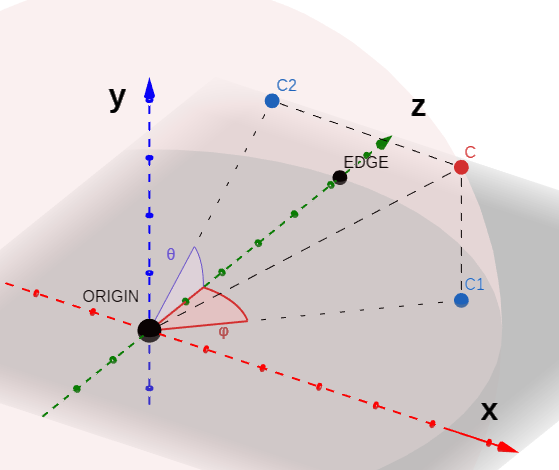
\includegraphics[width=0.9\linewidth]{img/video360/polar_coord.png}
        \caption{Polar coordinates example.}
        \label{fig:polar_coordinates}
    \end{subfigure}
    \begin{subfigure}[b]{0.49\linewidth}
    \centering
        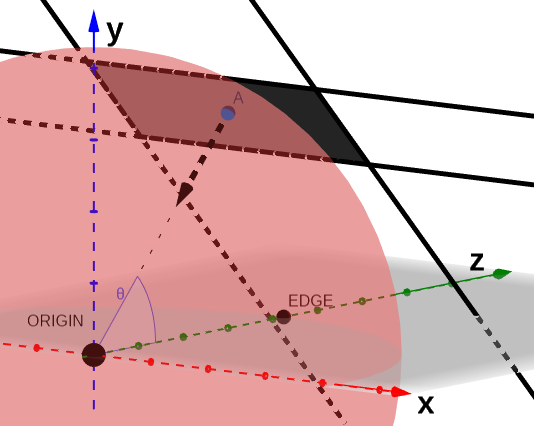
\includegraphics[width=0.9\linewidth]{img/video360/normal_vector.png}
        \caption{Element rotation example.}
        \label{fig:element_rotation}
    \end{subfigure}
    \caption{Polar coordinates system}
\end{figure}

The rotation of a media object is set in a
way that the normal vector on the center of its surface points to the origin.
%%
By doing so, in any position it is placed, the media object is always facing the viewer.
%%
Figure~\ref{fig:element_rotation} shows this rotation, where \emph{A} is the
center of the media object.

In the proposed model, each \emph{<scene360>} has always a main 360-degree
interactive video. 
%%
The initial scene in which the application starts is defined by an attribute
\emph{entry} in the element <body>. 
%%
This attribute refers to the \emph{id} attribute of the \emph{<scene360>}
element pointing to the main 360-degree video. 
%%
Media objects inside a 360 scene can be synchronized to main video~(\textbf{RP.6}).
%%
For this, we use SMIL \emph{begin} and \emph{dur} attributes in a media
object.
%%
They, respectively, define the start time and duration for the presentation of
the specified media object.

The \emph{onselect} attribute is used to support user navigation through 360
scenes~(\textbf{RI.1}).
%%
This attribute can be defined in any media element, by referencing the
\emph{id} of the target scene in its value.
%%
Once defined in an element, it transforms it into a navigation element for the
referenced scene.
%%
Moreover, the \emph{<preview>} defines a viewport of a \emph{<scene360>} using
its \emph{id} in the \emph{src}, which can be viewed as a 2D video inside
another scene.
%%
The temporal segment of the target scene displayed in the preview is defined
by the attributes \emph{clipBegin} and \emph{clipEnd}. 

The 360 video might have a particular region of interest to the viewer, which
is represented by the \emph{<hotspot>}~(\textbf{RI.2}) element.
%%
Britta~\cite{Britta2017} defines a hotspot as an interactive area in a video
that invoke an action.
%%
The author may create interactions when the user is either looking to it or
not.
%%
As in the other elements, its position is defined by the \emph{r, phi, theta}
attributes. 
%%
This element has also the attributes \emph{onLookAt} and
\emph{duringNotLookingAt}.
%%
The attribute \emph{onLookAt} specifies another element to be started once the
user looks at the \emph{<hotspot>}.
%%
Similarly, the attribute \emph{duringNotLookingAt} specifies another
element to be started when the user is not looking at the \emph{<hotspot>} and
is stopped once the user looks at it.

The \emph{<mirror>} element refers to picture-in-picture live view of a
viewport of the \emph{<scene360>} (\textbf{RI.3}).
%%
This viewport is defined using the \emph{src} attribute and assigning it to
the \emph{id} of a \emph{<hotspot>} element.
%%
Using these elements, authors can define that when the user is staring at a
viewport different from the one defined as a \emph{<hotspot>}, the
\emph{<mirror>} element will be triggered showing the PiP view at the current
user's viewport, attracting his attention to the important section of the
360-degree video.
%%
Since the \emph{<mirror>} element refers to a viewport of the current scene,
it does not support \emph{onselect} because it would not be intuitive to have
an element referring to a scene and navigating to another when selected.


\section{Dynamic Subtitles Positioning in 360-video}
\label{sec:authoring_discussion}

Using the adaptations described in Section \ref{sec:authoring_clustering_360}, we are able to apply \emph{video face clustering} in 360-videos. Figure \ref{fig:360_video_timeline} shows an example of this usage. It contains the two actors present in the 360-video and part of the video's timeline tagged with colors representing the presence of these actors.

\begin{figure}[!ht]
    \centering
    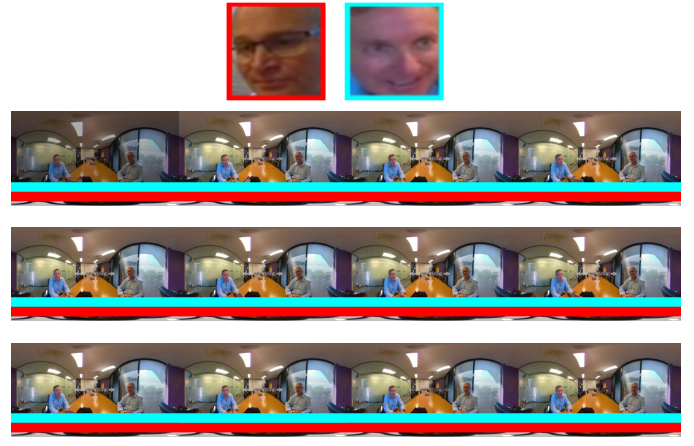
\includegraphics[width=0.8\linewidth]{img/video360/timeline-360.png}
    \caption{360-video timeline tagged by the actors presence. In this case, both actors were present in all frames.}
    \label{fig:360_video_timeline}
\end{figure}

With this clustering, for each actor detected, we generate a file containing the positions in polar coordinates of him/her for each time. By doing so, we use these files for defining the subtitles positioning using our authoring model. Listing \ref{list:ex-subtitles} shows the XML representation of an interactive 360-video with subtitles. In lines 6 and 7, we define subtitles elements, one for each actor. Using the \emph{tpos} attribute, we define that these subtitles follow the actors positions in the video. As the positions defined in the \emph{tpos} files are relative to the initial position of the subtitle element, we use \emph{theta}=5, so that the subtitles are placed 5 degrees bellow the center of the actors faces.


\begin{lstlisting}[
caption={XML representation for 360-video with subtitles following the actors positions.},
frameround=tttt,float=!ht, language=xml, 
label={list:ex-subtitles}, belowskip=-1\baselineskip, basicstyle=\footnotesize ]
<presentation360>
  <head>
  </head>
  <body entry = "boardroom">
    <scene360 id="boardroom" src="boardroom.mp4" volume="1">   
      <subtitle src="actor1.srt" r = "10" theta="5" tpos="actor1-positions.csv"/>      
      <subtitle src="actor2.srt" r = "10" theta="5" tpos="actor2-positions.csv"/>
    </scene360>
  </body>
</presentation360>
\end{lstlisting}

We can also define a more interactive setting for subtitles in 360-video with our authoring model and \emph{video face clustering}. In this new setting, the subtitles follow the actors when they are in the user's viewport, which means that the user can see them. When they are not visible, subtitles are presented at the bottom center of the user's viewport. Listing \ref{list:ex-interactive-subtitles} contains the definition of this setting. 

In the \emph{head}, we define three \emph{styles}. These \emph{styles} contain attributes that can be reused by the elements in the body. The first two \emph{styles}~(lines 3 and 4) define attributes regarding the actor positions in the 360-video with their respective times. These styles are used by the \emph{subtitle} elements on lines 9 and 10 for defining that such subtitles follow the actors positions. We also define two \emph{hotspot} elements that follow the actor positions~(lines 11 and 12). They are used like triggers with the attribute \emph{duringNotLookingAt} to start the other \emph{subtitles} when the \emph{hotspot} elements~(the actors) are not visible to the user. The other \emph{substile} elements reuse the style defined on line 5. This \emph{style} contains the attribute \emph{followCamera} set to \emph{true}, so that it follows the users head motion. In this way, the \emph{subtitles} defined on lines 13 and 14 follow the user's head motion.


\begin{lstlisting}[
caption={XML representation for 360-video with subtitles following the actors positions.},
frameround=tttt,float=!ht, language=xml, 
label={list:ex-interactive-subtitles}, belowskip=-1\baselineskip, basicstyle=\footnotesize ]
<presentation360>
  <head>
    <style id ="sty-actor1" tpos="actor1-positions.csv" begin="0s" r = "10"/>
    <style id ="sty-actor2" tpos="actor2-positions.csv" begin="0s" r = "10"/>
    <style id ="sty-follow" begin ="0s"  theta="20" followCamera="true" r="10"/>
  </head>
  <body entry = "boardroom">
    <scene360 id="boardroom" src="boardroom.mp4" volume="1">      
      <subtitle style="sty-actor1" src="actor1.srt" theta="5"/>      
      <subtitle style="sty-actor2" src="actor2.srt" theta="5"/>
      <hotspot style ="sty-actor1" duringNotLookingAt="sub-follow-actor1"/>
      <hotspot style ="sty-actor2" duringNotLookingAt="sub-follow-actor2"/>
      <subtitle style ="sty-follow" id="sub-follow-actor1" src="actor1.srt"/>
      <subtitle style ="sty-follow" id="sub-follow-actor2" src="actor2.srt"/>
    </scene360>
  </body>
</presentation360>
\end{lstlisting}

Figure \ref{fig:dynamic_subtitles} show how this setting works. In Figure \ref{subfig:subtitles_actor}, the subtitles are placed closed to the actor that is visible in the current user's viewport. When the actor is not visible, as shown in Figure \ref{subfig:subtitles_bottom}, the subtitles are placed at the bottom of the user's viewport. In this way, the user does not lose the content present on the subtitles.

\begin{figure}[!ht]
\centering
    \begin{subfigure}{0.47\linewidth}
        \centering
        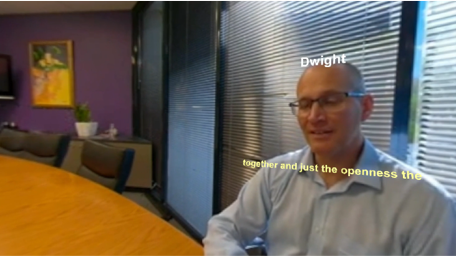
\includegraphics[width=1\textwidth]{img/video360/subtitles_actor.png}
        \caption{Subtitles close to actors' faces when they are in the user's viewport.}
        \label{subfig:subtitles_actor}
    \end{subfigure}\hfill
    \begin{subfigure}{0.47\linewidth}
        \centering
        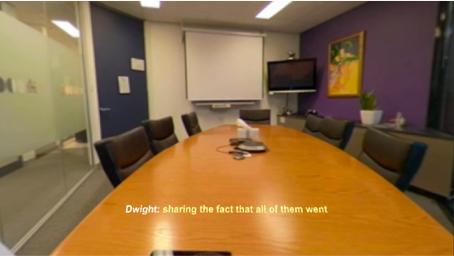
\includegraphics[width=1\textwidth]{img/video360/subtitles_bottom.png}
        \caption{Subtitles positioning in the bottom of user's viewport otherwise.}
        \label{subfig:subtitles_bottom}
    \end{subfigure}

\caption{Dynamic subtitles positioning using video face clustering and our authoring model.}
\label{fig:dynamic_subtitles}
\end{figure}

It is worth noticing that, with this setting, the disadvantage presented in Table \ref{tab:catalog} that the speaker-following subtitles are not always visible to user is mitigated.
%% -*- coding: utf-8 -*-
\newpage

\chapter{Conclusions}
\label{chap:conclusions}

In this dissertation, we present a method for spatio-temporal localization of actors based on \emph{Video Face Clustering}. As part of this method, we also define an algorithm for finding an adequate number of clusters based on the silhouette score. We investigate to what extent this method can be used as the core to leverage and enhance some innovative applications, especially in three different practical and important tasks: \emph{Video Face Recognition}, \emph{Educational Video Recommendation}, and \emph{Subtitles Positioning in 360-Video}.

For the \emph{Video Face Recognition}, we propose a cluster-matching-based approach, derived mainly by the characteristics of our core \emph{Video Face Clustering} method, which is very scalable since the effort spent with annotations is significantly reduced --- as it is done over clusters instead of single images. This method uses \emph{Video Face Clustering} and a heuristic for cluster matching to recognize people in videos. It has achieved a recall of 99.435\% and precision of 99.131\% when considering faces extracted from a set of 13 video files. As another consequence of face clustering, our technique can be useful for creating and labeling datasets in a less time-consuming way by labeling clusters instead of individual images. One of the limitations of this application is related to the size of the video set used for the overall evaluation of our method. This is due to the difficulty of finding videos where it is possible to manually identify in each frame whether each person present is registered or not in our labeled clusters.

For the \emph{Educational Video Recommendation} task, we investigate a new feature that can be used for such recommendation: the presence of specific lecturers, which again is a direct result of the application of our core method. After performing \emph{Video Face Clustering} on each video, we extract their centroids to perform another clustering step that creates a relationship of videos that share the presence of the same lecturers. Finally, we rank the recommended videos based on the amount of time that each lecturer is present. Our method uses only the video files for performing recommendations, no other information about these videos nor the identity of the lecturers is necessary. It is worth mentioning that we do not intend to substitute other video recommendation methods, rather our application shows that, if the presence of lecturers is a relevant feature for educational video recommendation, it can be used for this purpose with a mAP value of 0.99. The main limitation of this application is that we can only recommend videos in which the lecturers are visually present. As future work, we intend to investigate a hybrid recommendation approach, that combines both textual and audiovisual information from the video to create clusters.

For the \emph{Subtitles Positioning in 360-Video} task, our main contribution is the proposal of dynamic placement of subtitles based on the automatic localization of actors. To achieve this goal, we adapted our spatio-temporal localization method to the 360-video setting and created an authoring model for interactive 360-videos. Because of the severe distortions present in equirectangular 360-videos, we used an approach based on viewports extraction for the face detection step of \emph{Video Face Clustering}. To evaluate this approach against the sole use of a traditional CNN, we created a synthetic dataset by projecting images from the FDDB benchmark to equirectangular backgrounds. Our approach, which consists of using viewports with a traditional CNN, performed better than using the traditional CNN directly to the equirectangular images. Moreover, we proposed an authoring model that allows authors to design and create interactive 360 videos. The proposed model is the result of the analysis of different scenarios of immersive 360 multimedia applications. Besides supporting subtitles positioning in 360-videos, it also supports navigation among 360-videos, additional media, etc. 

In summary, we highlight the following contributions of this dissertation:
%%
\begin{enumerate}
    \item A method for video face recognition that is easily scalable and helps in labeling images dataset;
    \item A method for educational video recommendation based on the presence of lecturers;
    \item A method for face detection in equirectangular 360-images that uses models pre-trained with traditional images;
    \item A synthetic dataset for face detection in equirectangular 360-images;
    \item An authoring model for interactive 360-videos;
    \item A player for interactive 360-videos;
    \item An approach for automatic positioning subtitles in 360-videos based on the actors' positions;
\end{enumerate}

The choice for our three proposed applications was due to observations of opportunities to apply \emph{Video Face Clustering} in different contexts. We started with \emph{Video Face Recognition} task. We observed that the use of only the \emph{Video Face Clustering} part of the method could generate the time segments that each actor is present without having to identify them. Then, we hypothesized that this particular feature could also be used to clustering actors in different videos. From this observation, we decided to investigate a method for \emph{Educational Video Recommendation} using this clustering of actors in different videos. The idea for \emph{Subtitles Positioning in 360-video} came from the authoring model we developed. We observed that we could automatically identify the actors using \emph{Video Face Clustering} so that the subtitles could follow the speakers in the 360-video. Thus, we adapted \emph{Video Face Clustering} for the 360-video setting. It is worth noticing that with this adaptation, the other two applications~(\emph{Video Face Recognition} and \emph{Educational Video Recommendation}) could also be applied to the context of 360-videos.

This work has opened lots of branches for future research. For the particular case of subtitles positioning in 360-video, there is still much to explore. It is not yet clear what is the most adequate way to place subtitles relative to the actors' positions. For instance: is it better to place them above or below the actors' faces? Should the subtitles follow the actors immediately or it would be better to have a delay with a smooth transition? A path towards answering these questions is by experimenting and evaluating these and other possible settings with users.

Other possible future work comes from the combination of the applications we explored in this dissertation. For instance, the identification of lecturers using a lecturer's image dataset with \emph{Video Face Recognition} could improve the task of \emph{Educational Video Recommendation} by inserting additional relationships among lecturers~(e.g. lecturers that teach the same subject). Another possibility is to use \emph{Video Face Recognition} to identify and insert the name of the actor present in 360-videos together with the subtitles so that the users know who is talking when the actor is not visible to them.

Although this dissertation has focused on faces, the methods and techniques here investigated could also be applied in other contexts. For instance, we could recommend videos based on the presence of the same \emph{actions} in different videos, so that a reference video with many actions related to culinary, for example, such as pouring and chopping should have videos with similar \emph{actions} as recommended. For doing that, we should be able to represent each action identified as an embedding~(vector). Then, the remainder of our method for \emph{Educational Video Recommendation} could be used. In the context of 360-videos, if we could generate art embeddings from pieces of art, we could apply the process of \emph{Video Face Clustering}~(or \emph{Video Art Clustering} in this case) to detect and determine the video segments that each piece of art is present. In this case, instead of using \emph{CNNs} trained for detecting and generating embeddings for faces, we would use them for pieces of art. By doing that, we would be able to use our authoring model to attach additional media such as text and audio to pieces of art in an interactive 360-video. This application could be useful in the context of virtual tours in museums and historical sites.


\section{Publications}

 As a result of this research, three papers have already been published at relevant multimedia conferences \cite{mendes2020cluster,mendes2020ISM, mendes2020authoring}. In \cite{mendes2020cluster}, we have evaluated video face clustering together with a cluster-matching method for video face recognition. In \cite{mendes2020ISM}, we have used video face clustering and the presence of actors in different videos as a means for recommending educational videos. In \cite{mendes2020authoring}, we have developed an authoring model and a player for interactive 360-video. 

\arial
\bibliography{references}

% Apendix chapters below.
%\normalfont
%\appendix
%\newpage

\chapter{User profile questionnaire for prototype evaluation sessions}
\label{chap:profile-form}

\begin{enumerate}
\item Personal information
  \begin{enumerate}
 \item Name
 \newline \rule[0pt]{300pt}{1pt}
 \item E-mail
 \newline \rule[0pt]{300pt}{1pt}
 \item Education degree
 \newline \rule[0pt]{300pt}{1pt}
 \item Course semester (just for students)
 \newline \rule[0pt]{300pt}{1pt}
 \item Occupation
 \newline \rule[0pt]{300pt}{1pt}
  \end{enumerate}
\item Please mark below your knowledge about the following subjects:
	\begin{enumerate}
   \item Division of a sample by percentiles: P10, P50, P80 ...
		\newline \circle{10} I do not know
     \newline \circle{10} I know little (I have learned these concepts at some point, but may have to learn again if I have to apply them)
     \newline \circle{10} I have average knowledge (I may have to revise one concept or another if I have to apply it)
     \newline \circle{10} I know well (I do not apply often, but I would not need to revise the concepts if I had to apply them)
     \newline \circle{10} I am a specialist (I apply these concepts frequently)
	  \newline 
   \item Analysis of trends and patterns in time series
   \newline \circle{10} I do not know
   \newline \circle{10} I know little (I have learned these concepts at some point, but may have to learn again if I have to apply them)
   \newline \circle{10} I have average knowledge (I may have to revise one concept or another if I have to apply it)
   \newline \circle{10} I know well (I do not apply often, but I would not need to revise the concepts if I had to apply them)
   \newline \circle{10} I am a specialist (I apply these concepts frequently)\\
      
   \item Projection chart (Time-lapsed LAMP chart)
   \begin{figure}[H]
		\centering
		\includegraphics[width=0.9\columnwidth]{images/form-timelapsedchart.png}
		\label{fig:form-timelapsedchart}
	   \end{figure}

   \circle{10} I do not know
   \newline \circle{10} I know little (I have learned these concepts at some point, but may have to learn again if I have to apply them)
   \newline \circle{10} I have average knowledge (I may have to revise one concept or another if I have to apply it)
   \newline \circle{10} I know well (I do not apply often, but I would not need to revise the concepts if I had to apply them)
   \newline \circle{10} I am a specialist (I apply these concepts frequently)\\

 \newpage
       \item Ranking chart (Bump chart)
       \begin{figure}[H]
 		\centering
 		\includegraphics[width=0.9\columnwidth]{images/form-bumpchart.png}
 		\label{fig:form-bumpchart}
 	   \end{figure}
       
       \circle{10} I do not know
       \newline \circle{10} I know little (I have learned these concepts at some point, but may have to learn again if I have to apply them)
       \newline \circle{10} I have average knowledge (I may have to revise one concept or another if I have to apply it)
       \newline \circle{10} I know well (I do not apply often, but I would not need to revise the concepts if I had to apply them)
       \newline \circle{10} I am a specialist (I apply these concepts frequently)\\

 \newpage
       \item Distance chart
       \begin{figure}[H]
 		\centering
 		\includegraphics[width=0.9\columnwidth]{images/form-distancechart.png}
 		\label{fig:form-distancechart}
 	   \end{figure}
      
       \circle{10} I do not know
       \newline \circle{10} I know little (I have learned these concepts at some point, but may have to learn again if I have to apply them)
       \newline \circle{10} I have average knowledge (I may have to revise one concept or another if I have to apply it)
       \newline \circle{10} I know well (I do not apply often, but I would not need to revise the concepts if I had to apply them)
       \newline \circle{10} I am a specialist (I apply these concepts frequently)\\

 \newpage
       \item Fanchart
       \begin{figure}[H]
 		\centering
 		\includegraphics[width=0.9\columnwidth]{images/form-fanchart.png}
 		\label{fig:form-fanchart}
 	  \end{figure}
      
       \circle{10} I do not know
       \newline \circle{10} I know little (I have learned these concepts at some point, but may have to learn again if I have to apply them)
       \newline \circle{10} I have average knowledge (I may have to revise one concept or another if I have to apply it)
       \newline \circle{10} I know well (I do not apply often, but I would not need to revise the concepts if I had to apply them)
       \newline \circle{10} I am a specialist (I apply these concepts frequently)

     \end{enumerate}
\end{enumerate}

\bibliographystyle{bibstyles/IEEEtran}

\end{document}